\documentclass[a4paper]{report}

\usepackage{../mathstemplate}
\usepackage{color}

\date{IV семестр, весна 2024 г.}
\title{Математический анализ. Неофициальный конспект}
\author{Лектор: Сергей Витальевич Кисляков \\ Конспектировал Леонид Данилевич}

\begin{document}
    \shorthandoff{"}
    \maketitle
    \tableofcontents
    \newpage
    \setcounter{lection}{0}
    \chapter{Комплексный анализ}
    \newlection{16 февраля 2024 г.}
    Пусть $f: G \map \C$, где открытое $G \subset \C$.
    \definition[$f$ голоморфна в $z_0 \in G$]{
    $\exists \lim\limits_{z \to z_0}\frac{f(z) - f(z_0)}{z - z_0} \bydef f'(z_0)$.
    }
    Во втором семестре мы проверяли, что $f = u + iv$ (где $u, v: G \map \R$) голоморфна в $z_0 \iff f$ дифференцируема в вещественном смысле, и выполняются уравнения Коши --- Римана:
    \encircle{\der{u}{x} = \der{v}{y} \qquad \der{u}{y} = -\der{v}{x}}
    \definition[$f$ аналитична в $G$] {
    $\forall z_0 \in G: \exists c_j \in \C$: \[f(z) = \sum\limits_{j = 0}^{\infty}c_j(z - z_0)^j\tag{$*$}\label{analytic}\] где ряд сходится не только при $z = z_0$.
    }
    \theorem{\label{analytic-is-holomorphic}
    $f$ аналитична в $G \iff f$ голоморфна во всех точках $G$.
    \provetwhen{
        Доказали во втором семестре, несложно.
    }{
        Скоро займёмся, время пришло.
    }
    }
    Из представления~(\ref{analytic}) следует, что производная в точке $z$ считается почленно: $f'(z) = \sum\limits_{j = 1}^{\infty}j c_j (z - z_0)^{j - 1}$.
    В частности, отсюда получается, что $f'(z_0) = c_1$, и вообще $f^{(n)}(z_0) = j! \cdot c_j$.

    Вскоре мы увидим, что ситуация разительно отличается от вещественной: в вещественном случае были разные классы --- дифференцируемые функции, $C^1$, $C^\infty$, аналитичные, и множество промежуточных классов.

    В комплексном же случае, если функция хотя бы один раз дифференцируема, то окажется, что этого достаточно, чтобы она была не просто дифференцируема, а непрерывно дифференцируема, бесконечно дифференцируема, и даже аналитична.
    \section{Интеграл от дифференциальной формы вдоль кусочно-гладкого пути}
    \subsection{Про дифференциальные формы}
    \definition[Линейная функция $l: \R^n \map \C$]{${\forall \alpha, \beta \in \R, x, y \in \R^n: l(\alpha x + \beta y) = \alpha l(x) + \beta l(y)}$.}
    \definition[Линейная форма на множестве $G \subset \R^n$]{
    Функция двух переменных ${\phi: G \times \R^n \map \C}$, линейная по второму аргументу.
    }
    В пространстве $\R^n$ имеется базис $(e_j)$: $h = e_1 h_1 + \dots + e_n h_n$.

    Тем самым, $\phi(x, h) = \sum\limits_{j = 1}^{n}\underbrace{\phi(x, e_j)}_{\eqqcolon g_j(x)}h_j = \sum\limits_{j = 1}^{n}g_j(x)h_j$.

    Введём \emph{базисные линейные формы} $\d x_j(u, h) = h_j$, игнорирующую первую координату, и возвращающая $j$-ю компоненту второго аргумента.
    Теперь $\phi(x, h)$ разложилась в сумму $\sum\limits_{j = 1}^{n}g_j \d x_j$.

    \example{
        Пусть $f: G \map \C$ --- дифференцируемая в $G$ функция.
        Заметим, что её дифференциал $\d_f(x, \_)$ --- в точности линейная форма на $G$.

        При разложении по базису получится $\d_f(x, \_) = \sum\limits_{j = 1}^{n}\der{f}{x_j}(x)\d x_j$.
    }
    Вскоре мы увидим, что далеко не всякая линейная форма является чьим-то дифференциалом.

    Если $\phi = \sum\limits_{j = 1}^{n} g_j\d x_j$ --- дифференциал функции $f$, то непременно $g_j = \der{f}{x_j}$.

    Тот факт, что $\phi$ является дифференциалом $f$, можно сказать наоборот: $f$ является первообразной $\phi$.
    \subsection{Про интегрирование}
    Рассмотрим монотонную функцию $\Phi: \angles{a, b} \map \R$.
    Как и при определении стилтьесовой длины, будем считать, что $\Phi$ определена на некотором открытом множестве, содержащем $\angles{a, b}$.
    Обозначим за $l_\Phi$ стилтьесову длину, отвечающую функции $\Phi$.

     Пускай $\lambda_\Phi$ --- продолжение стилтьесовой длины $l_\Phi$ по Лебегу --- Каратеодори.

    Она, как водится, определена на некоторой $\Sigma$-алгебре, в которой есть борелевские множества, но измеримы могут быть и какие-то другие множества, зависящие от конкретной функции $\Phi$.
    \examples{
        \item Так, функция $\phi(x) = \all{0,&x < 0 \\ 1,& x \ge 0}$ порождает дельта-меру $\delta_0$, относительно которой все множества измеримы.

        Кроме того, эта мера сингулярна относительно стандартной меры Лебега.

    \item Может показаться, что так происходит из-за разрывности $\phi$, но это не так.

        Рекурсивно определим канторову лестницу $C: [0, 1] \map [0, 1]$:
        \[\begin{tikzpicture}[scale=1]
              \draw[->] (-0.5,0) -- (3.5,0) node[above]{$x$};
              \draw[->] (0,-0.5) -- (0,3.5) node[right]{$y$};
              \fill (0, 0) circle (1.5pt) node[below left] {$0$};
              \fill (1, 0) circle (1.5pt) node[below] {$\nicefrac13$};
              \fill (2, 0) circle (1.5pt) node[below] {$\nicefrac23$};
              \fill (3, 0) circle (1.5pt) node[below] {$1$};
              \fill (0,1.5) circle (1.5pt) node[left] {$\nicefrac12$};
              \fill (0,3) circle (1.5pt) node[left] {$1$};
              \newcommand{\cantor}[5]{ %l, r, d, u, depth
                  \pgfmathsetmacro{\depth}{\numexpr#5}

                  \draw ({(#1+2*#2)/3},{(#3+#4)/2}) -- ({(2*#1+#2)/3},{(#3+#4)/2});

                  \ifnum\depth<5
                  \cantor{#1}{(2*#1+#2)/3}{#3}{(#3+#4)/2}{#5+1}
                  \cantor{(#1+2*#2)/3}{#2}{(#3+#4)/2}{#4}{#5+1}
                  \else
                  \draw ({#1}, {#3}) -- ({#2}, {#4});
                  \fi
              }
              \cantor{0}{3}{0}{3}{0}
        \end{tikzpicture}\]
        Построив по данной функции стилтьесову длину $\lambda_C$, мы получим меру, сосредоточенную на канторовом множестве меры нуль.

        Её носитель --- само канторово множество, так как на всех отрезках вне канторова множества $\lambda_C$ равна нулю.
        Она сингулярна относительно стандартной меры Лебега на $\R$, и её измеримые множества разительно отличаются от измеримых множеств меры Лебега.
    }
    По мере Стилтьеса можно интегрировать: если $v$ является $\lambda_\Phi$ измеримой (в частности, измерима по Борелю и непрерывна), то определён интеграл $\int\limits_{\angles{a, b}}v \d\lambda_{\Phi}$
    Иногда пишут просто $\int\limits_{\angles{a, b}}v \d \Phi$. %Так складывается ощущение, что из измеримости следуют и борелевская измеримость, и непрерывность. % ок, заменю "и даже" на "и"
    \ok
    Теперь пусть $I = [a, b]$, и $\Psi: [a, b] \map \R$ --- функция ограниченной вариации.
    В таком случае $\Psi = \Phi_1 - \Phi_2$, где некие $\Phi_1, \Phi_2$ возрастают.
    Можно определить знакопеременную меру $\lambda_\Psi \bydef \lambda_{\Phi_1} - \lambda_{\Phi_2}$, понятно, что определение корректно.
    \subsection{Интеграл от дифференциальной формы вдоль пути}
    Пускай $\gamma: [a, b] \map G \subset \R^n$ --- спрямляемый путь (путь конечной длины).
    Пускай $U = \sum\limits_{j = 1}^{n}u_j \d x_j$ --- дифференциальная форма в области $G$.
    Если не сказано противное, будем считать, что $u_j$ --- непрерывные функции.
    \definition[Интеграл от $U$ вдоль пути $\gamma$]{\label{piecewise-smooth-integral}
    $\int\limits_{\gamma}U \bydef \sum\limits_{j = 1}^{n}\int\limits_{[a, b]}u_j(\gamma(t))\d \gamma_j(t)$.
    }
    Здесь $\gamma = (\gamma_1, \dots, \gamma_n)$.
    Так как путь спрямляем, то все $\gamma_j$ --- ограниченной вариации, каждая порождает свою меру Стилтьеса, и определение интегрирует композицию $U \circ \gamma$ по данной мере.
    \subsection{Сумма путей}
    Пускай имеются два отрезка $[a, c]$ и $[c, d]$, и на них заданы пути $\gamma_1: [a, c] \map G$, $\gamma_2: [c, d] \map G$.
    Предположим, что $\gamma_1(c) = \gamma_2(c)$.

    Тогда можно устроить путь $\gamma = \gamma_1 \oplus \gamma_2: [a, d] \map G$, $\gamma(t) \bydef \all{\gamma_1(t),&t \in [a, c] \\ \gamma_2(t),& t \in [c, d]}$.

    \note{
    Интеграл аддитивен по множеству: $\int\limits_{\gamma_1 \oplus \gamma_2}U = \int\limits_{\gamma_1}U + \int\limits_{\gamma_2}U$. %Мб тут вставить ", поэтому", а тто так не выглядит, как по множеству.
    }
    \subsection{Альтернативное определение}
    Далее мы не интересуемся никакими чудесами вроде канторовых лестниц, и считаем, что $\Phi$ такова, что $\lambda_\Phi$ абсолютно непрерывна относительно стандартной меры Лебега.

    А раз так, то по теореме Радона --- Никодима $\exists$ суммируемая $w: [a, b] \map \R$, такая, что \[\lambda_\Phi(e) = \int\limits_{e}w(x)\d x\tag{$+$}\label{density}\]
    \fact{\label{density-is-derivative}
        Формула~(\ref{density}) заведомо верна, если $\Phi$ непрерывно дифференцируема на $[a, b]$, тогда $w = \Phi'$.
        \provehere{
            Введём меру $\nu(e) = \int\limits_{e}\Phi'(x)\d x$, заданную на измеримых по Лебегу множествах.
            $\Phi'$ непрерывна, и, следовательно, измерима.

            Если $\angles{c, d} \subset [a, b]$, то $\nu(\angles{c, d}) = \int\limits_{\angles{c, d}}\Phi'(x)\d x = \Phi(d) - \Phi(c) = l_\Phi(\angles{c, d})$.

            Таким образом, из теоремы единственности, продолжение $l_\Phi$ по Лебегу --- Каратеодори совпадает с $\int\limits_{e}\Phi'(x)\d x$.
        }
    }
    \note{
        Утверждение~(\cref{density-is-derivative}) сохраняет силу, если $\Phi$ непрерывна и кусочно-непрерывно дифференцируема.
    }
    \comment{Далее где-то используется $\Phi$, а где-то $\beta$, надо убедиться, что это везде одно и то же, и заменить. } % тогда и я трогать эти две буквы пока не буду
    Пускай $\beta: [a, b] \map \R$ --- функция ограниченной вариации, кусочно-непрерывно дифференцируемая: $\exists a = a_0 < a_1 < \dots < a_k = b$, такие, что $\beta$ непрерывно дифференцируема на $[a_s, a_{s+1}]$ при $0 \le s < k$.
    Введём $\rho(e) = \int\limits_{e}\beta'(x)\d x$ --- это знакопеременная вещественная мера.

    У данной меры возникают (см. разложение Хана) положительная и отрицательная части $\rho_+(e) \bydef \int\limits_{e}(\beta')_+(x)\d x$ и $\rho_-(e) \bydef \int\limits_{e}(\beta')_-(x)\d x$
    
    Если обозначить за $\Phi_+(t) = \int\limits_{0}^{t}(\beta')_+(x)\d x$ и $\Phi_-(t) = \int\limits_{0}^{t}(\beta')_-(x)\d x$, то окажется, что соответствующие меры Стилтьеса совпадают с $\rho_+$ и $\rho_-$.
    
    Более того, $\beta = \Phi_+ - \Phi_-$ --- получили разложение функции ограниченной вариации в положительную и отрицательную части.
    \note{
    Это разложение экономнее, чем то, которое было получено ранее --- ранее в качестве $\Phi_+$ выбиралась вариация $\Phi$.
    }
    
    Если всё, что написано выше, собрать вместе, то получится 
    \encircle{\int\limits_{[s, t]}v \d \Phi = \int\limits_{[s, t]}v(x)\beta'(x)\d x}
    Далее <<гладкий>> используется, как синоним к непрерывно-дифференцируемому.
    \corollary[Можно считать определением]{
        Если $U = \sum\limits_{j = 1}^{n}u_j \d x_j$ --- дифференциальная форма в $G$ с непрерывными коэффициентами, а $\gamma = (\gamma_1, \dots, \gamma_n): [a, b] \map G$ --- спрямляемый кусочно-гладкий путь, то
    \[\int\limits_{\gamma}U = \sum\limits_{j = 1}^{n}\int\limits_{a}^{b}u_j(\gamma(t))\gamma_j'(t)\d t\]
    }
    \subsection{(Не)зависимость от параметризации}
    Пускай $\gamma: [a, b] \map G$ --- кусочно-гладкий путь, $\psi: [c, d] \map [a, b]$ --- гладкий гомеоморфизм.

    Теперь $\tilde{\gamma} = \gamma \circ \psi$ --- перепараметризация $\gamma$
    \lemma{
        Для всякой формы $U$:
        \[\int\limits_{\tilde{\gamma}}U = \pm\int\limits_{\gamma}U\]
        Знак $+$ выбирается, если $\psi$ возрастает, и $-$ --- если убывает.
        \provehere{
            Предположим, что $\gamma$ --- гладкий путь, иначе применяем к кусочкам гладкости по отдельности.

            $\int\limits_{\tilde{\gamma}}U = \sum\limits_{j = 1}^{n}\int\limits_{c}^{d}u_j(\gamma(\psi(t)))\gamma_j'(\psi(t))\cdot \psi'(t)\d t = \left\|\arr{c}{\tau = \psi(t) \\ \d \tau = \psi'(t)\d t}\right\| = \sum\limits_{j = 1}^{n}\int\limits_{\psi(c)}^{\psi(d)}u_j(\gamma(\tau))\gamma_j'(\tau)\d \tau = \pm \int\limits_{\gamma}U$
        }
    }
    Про $\psi$ также можно считать, что это он не гладкий, а лишь кусочно-гладкий.

    Тем самым, можно определить сумму путей для несоприкасающихся отрезков: для двух путей $\gamma_1: [a, b] \map G, \gamma_2: [c, d] \map G$ (при условии $\gamma_{1}(b) = \gamma_2(c)$) можно один их отрезков-прообразов линейным возрастающим преобразованием перевести в отрезок, соприкасающийся со вторым (например, $t \mapsto t + (b - c)$).

    Также есть понятие обратного пути $\gamma^-(t) = \gamma(a + b - t)$.
    Для любой формы $U$: \[\int\limits_{\gamma \oplus \gamma^-}U = \int\limits_{\gamma}U + \int\limits_{\gamma^-}U = \int\limits_{\gamma}U - \int\limits_{\gamma}U = 0\]
    \section{Условия существования первообразной у дифференциальной формы}
    \theorem{
    Если у дифференциальной формы $U$ в открытом множестве $G \subset \R^n$ имеется первообразная $F$, то для всякого кусочно-гладкого пути $\gamma: [a, b] \map G$
    \[\int\limits_{\gamma}U = F(\gamma(b)) - F(\gamma(a))\]
    \provehere{
        $U = \sum\limits_{j = 1}^{n}g_j \d x_j$, где $g_j(w) = \der{}{x_j}F(w)$.
        Считаем, что путь гладкий.
    \[\int\limits_{\gamma}U = \sum\limits_{j = 1}^{n}\int\limits_{a}^{b}\der{}{x_j}F(\gamma(t))\gamma_j'(t)\d t = \int\limits_{a}^{b}\frac{\d}{\d t}(F \circ \gamma)(t)\d t = F(\gamma(b)) - F(\gamma(a))\]
    Если же путь всего лишь кусочно-гладкий, то надо разбить отрезок на подотрезки гладкости, и сложить.
    }
    }
    \corollary{
    Если у дифференциальной формы $U$ есть первообразная, то её интегралы по всем путям с данными началом и концом, равны.
    }
    Оказывается, верно и обратное.
   %Надо пересмотреть написание "кусочно-непрерывно дифференцируемый", я нашёл вариант с двумя дефисами.
    \newlection{26 февраля 2024 г.}
    \lemma{
        Пусть $G$ --- область в $\R^n$, тогда любые две её точки можно соединить ломаной (кусочно-линейным путём).
    \provehere{
        Выберем $x_0 \in G$, положим $U = \defset{y \in G}{\text{существует ломаная в $G$ с началом в $x_0$ и концом в $y$}}$.

        Покажем, что $U$ открыто.
        Пусть $y \in U$, тогда найдётся шарик $B_\eps(y) \subset G$, и $B_\eps(y) \subset U$ --- можно добавить одно звено к ломаной $x_0 \rightsquigarrow y$.

        Покажем, что $U$ замкнуто.
        Пусть $z \in G$ --- предельная точка для $U$. Найдётся $B_\eps(z) \subset G$, так как $z$ --- предельная, то $\exists y \in B_\eps(z) \cap U$.
        Значит, $z \in U$ --- можно добавить одно звено $y \rightarrow z$.
    }
    }
    \note{
        Имея кусочно-линейный путь $\gamma: [a, b] \map G$, соединяющий $A,B \in G$, несложно получить бесконечно дифференцируемый путь, соединяющий их:

        Пусть $\gamma_1: [a - 1, b + 1] \map G, \gamma_1(t) = \all{\gamma(t),&t \in [a, b] \\ \gamma(a),& t \in [a-1, a] \\ \gamma(b),&t \in [b, b + 1]}$.
        Теперь, сворачивая $\gamma_1$ с аппроксимативной единицей с достаточно большим номером и достаточно малым компактным носителем, получим бесконечно дифференцируемый путь, соединяющий $A$ и $B$.
    }
    \theorem{\label{integral-along-path}
        Пусть $\Phi = \sum\limits_{j = 1}^{n}f_j(x)\d x_j$ --- \emph{непрерывная} дифференциальная форма в $G$ (то есть коэффициенты непрерывны в $G$).
        Следующие условия эквивалентны.
        \numbers{
        \item У $\Phi$ есть первообразная $F$, то есть функция $F \in C^1(G): \d F = \Phi$ (иными словами, $\forall j: \der{}{x_j}F = f_j$).
        \item Для всех кусочно-гладких путей $\gamma$ с фиксированными началом и концом $\gamma(a) = \gamma_a, \gamma(b) = \gamma_b$: $\int\limits_{\gamma}\Phi$ не зависит от $\gamma$ (а только от начала и конца).
        \item Для любой кусочно-гладкой петли (то есть замкнутого пути) $\gamma$ в $G$:  $\int\limits_{\gamma}\Phi = 0$.
        }
%        такова, что $\forall x, y \in G: \exists c \in \C: \forall$ кусочно-гладкого пути $\gamma$ с началом в $x$ и концом в $y$: $\int\limits_{\gamma}U = c$.
%        Эквивалентно, для всех замкнутых кусочно-гладких путей $\gamma: \int\limits_{\gamma}U = 0$.

%        Тогда $U$ обладает первообразной.
        \provehere{
            Мы уже доказали ранее цепочку импликаций $(1) \then (3) \then (2)$. Далее доказываем $(2) \then (1)$.

            Предъявим кандидат в первообразную.
            Зафиксируем $x_0 \in G$, выберем $x \in G$, пусть $\gamma$ --- произвольный кусочно-гладкий путь с началом в $x_0$ и концом в $x$.
            Определим $F(x) \bydef \int\limits_{\gamma}\Phi$.
            Согласно посылке, $F$ корректно определена --- не зависит от выбора пути.

            Покажем, что частные производные $F$ существуют, и равны $f_j$.
            Тогда они получатся непрерывными, то есть $F$ --- дифференцируемой, и окажется, что $F$ --- первообразная $\Phi$.

            Пусть $e_1, \dots, e_n$ --- стандартные базисные орты в $\R^n$.
            Рассмотрим $\frac{F(x + t e_j) - F(x)}{t}$.

            При малых $t$: отрезок между $x$ и $x + t e_j$ лежит внутри $G$.
            Пусть $\gamma_1$ --- путь, соединяющий $x_0$ и $x$, $l$ --- отрезок от $x$ до $x + t e_j$.
        \[\frac{F (x + te_j) - F(x)}{t} = \frac{1}{t}\left(\int\limits_{\gamma_1 \oplus l}\Phi - \int\limits_{\gamma_1}\Phi\right) = \frac{1}{t}\int\limits_{l}\Phi = \frac1t \int\limits_{0}^{t}f_j(x + \tau e_j)\d \tau \underset{t \to 0}\Map f_j(x)\qedhere\]
        }
    }
    \definition[Прямоугольник на плоскости]{
    Множество вида $[a, b] \times [c, d] \subset \R^2$.
    }
    Область $G$ на плоскости будем называть \emph{удобной}, если $\exists x_0 \in G: \forall y \in G: \exists$ прямоугольник $P \subset G$, содержащий точки $x$ и $y$.
    \examples[Удобные области]{
    \item $\Int Q$, если $Q$ --- прямоугольник. В качестве центра $x_0$ подойдёт любая точка.
    \item $B_r(x_0) = \defset{x \in \R^2}{|x - x_0| < r}$. В качестве центра $x_0$ стоит взять центр, иначе не получится:
    \[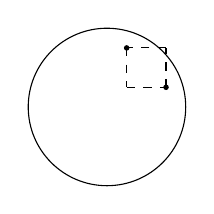
\begin{tikzpicture}
          \draw (0, 0) circle [radius=1];
          \fill (0.25,0.75) circle (1pt);
          \fill (0.75,0.25) circle (1pt);
          \draw[dashed] (0.25,0.75) -- (0.25, 0.25);
          \draw[dashed] (0.25,0.25) -- (0.75, 0.25);
          \draw[dashed] (0.75,0.25) -- (0.75, 0.75);
          \draw[dashed] (0.75,0.75) -- (0.25, 0.75);
    \end{tikzpicture}\]
    }
    \definition[Ориентированная граница прямоугольника $P$]{
    Петля $\gamma$, обходящая границу $P = [a, b] \times [c, d]$ против часовой стрелки, то есть вот так:
    \[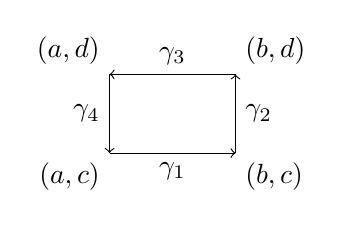
\begin{tikzpicture}
          \draw (0,0) node[below left] {$(a, c)$};
          \draw (0,1) node[above left] {$(a, d)$};
          \draw (1.6,0) node[below right] {$(b, c)$};
          \draw (1.6,1) node[above right] {$(b, d)$};

          \node at (0.8,0) [below] {$\gamma_1$};
          \node at (1.6,0.5) [right] {$\gamma_2$};
          \node at (0.8,1) [above] {$\gamma_3$};
          \node at (0,0.5) [left] {$\gamma_4$};

          \draw[->] (0,0) -- (1.6, 0);
          \draw[->] (1.6,0) -- (1.6, 1);
          \draw[->] (1.6,1) -- (0, 1);
          \draw[->] (0,1) -- (0, 0);
    \end{tikzpicture}\]
    $\gamma = \gamma_1 \oplus \gamma_2 \oplus \gamma_3 \oplus \gamma_4$.
    }
    Для прямоугольника $P$ будем обозначать за $\partial P$ в зависимости от контекста либо границу $P$, как топологического подмножества $\R^2$, либо путь, обходящий границу $P$ против часовой стрелки.
    \corollary[Дополнение к~(\cref{integral-along-path})]{
        Если $G$ --- удобная область на плоскости, то к трём эквивалентным условиям~(\cref{integral-along-path}) можно добавить
    \numbers{
    \item[4.] $\forall P \subset G: \int\limits_{\partial P}\Phi = 0$.
    }
    \provehere{
    $(3) \then (4)$ ясно, докажем $(4) \then (1)$.

    Пусть $x_0 \in G$ --- центр удобной области, определим $F(x) = \int\limits_{\delta}\Phi$, где $\delta$ --- это либо $\delta_1 \coloneqq \gamma_1 \oplus \gamma_2$ либо $\delta_2 \coloneqq \gamma_4^- \oplus \gamma_3^-$ (вне зависимости от выбора $\delta$ получится одно и то же).
        \[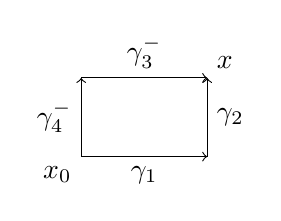
\begin{tikzpicture}
              \draw (0,0) node[below left] {$x_0$};
              \draw (1.6,1) node[above right] {$x$};

              \node at (0.8,0) [below] {$\gamma_1$};
              \node at (1.6,0.5) [right] {$\gamma_2$};
              \node at (0.8,1) [above] {$\gamma_3^-$};
              \node at (0,0.5) [left] {$\gamma_4^-$};

              \draw[->] (0,0) -- (1.6, 0);
              \draw[->] (1.6,0) -- (1.6, 1);
              \draw[<-] (1.6,1) -- (0, 1);
              \draw[<-] (0,1) -- (0, 0);
        \end{tikzpicture}\]
    Далее, чтобы проверить $\der{}{x_1}F = f_1$ и $\der{}{x_2}F = f_2$, воспользуемся подходящим представлением: пусть орт выглядит так: % "орт" --- это один, что тут имеется ввиду? "пусть орты расположены так"?
        \[\begin{tikzpicture}[scale=1]
            \draw[->](0,0) -- (0,1) node [below left] {$x_1$};
            \draw[->](0,0) -- (1,0) node [below left] {$x_2$};
        \end{tikzpicture}\]
        тогда для проверки $\der{}{x_1}F = f_1$ удобно воспользоваться определением $F$ через $\delta_1$, для проверки $\der{}{x_2}F = f_2$ --- определением через $\delta_2$. Далее повторяем рассуждение из (\cref{integral-along-path}).
    }
    }
    Пусть $\Phi = \sum\limits_{j = 1}^{n}f_j(x)\d x_j$ --- непрерывная дифференциальная форма в области $G \subset \R^n$.
    \definition[Форма $\Phi$ точна]{Существует первообразная $F$ в $G: \d F = \Phi$. }
    \definition[Форма $\Phi$ замкнута]{ Форма $\Phi$ локально точна ($\forall x_0 \in G: \exists U \ni x_0$: $\Phi\big|_U$ точна). }
    Понятно, что точная форма замкнута, но точность из замкнутости не следует: чуть позднее мы определим $\d z$, и покажем, что $\frac{\d z}{z}$ --- замкнутая, но не точная форма на $\C \sm \{0\}$
    \theorem{
    Пусть $\Phi$ --- дифференциальная форма в области $G \subset \R^n$.
        Следующие условия эквивалентны:
    \numbers{
    \item $\Phi$ замкнута.
    \item $\forall x_0 \in G: \exists V \ni x_0: \forall$ кусочно-гладкого замкнутого пути $\gamma$ с носителем в $V$: $\int\limits_{\gamma}\Phi = 0$.
    }
    Если $n = 2$, то дополнительно появляются ещё два условия:
    \numbers{
    \item[3.] $\forall z \in G: \exists \underset{\ni z}{V_z} \subset G: \forall P \subset V_z: \int\limits_{\partial P}\Phi = 0$.
    \item[4.] $\forall P \subset G: \int\limits_{\partial P}\Phi = 0$.
    }
    \provehere{
    Докажем, что $(3) \then (4)$, остальное уже доказано выше.

    Заметим, что границу прямоугольника $P$ можно представить, как сумму границ четырёх прямоугольников вдвое меньшего диаметра:
        \[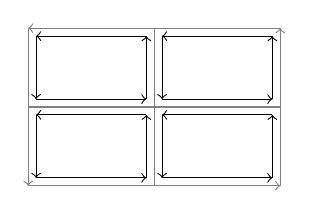
\begin{tikzpicture}
              \draw[->,color=gray] (0,0) -- (3.2, 0);
              \draw[->,color=gray] (3.2,0) -- (3.2, 2);
              \draw[->,color=gray] (3.2,2) -- (0, 2);
              \draw[->,color=gray] (0,2) -- (0, 0);
              \draw[color=gray] (0,1) -- (3.2,1);
              \draw[color=gray] (1.6,0) -- (1.6,2);
              \foreach \x/\y in {0/0,1.6/0,0/1,1.6/1} {
                  \draw[->] ({\x+0.1},{\y+0.1}) -- ({\x+1.5}, {\y+0.1});
                  \draw[->] ({\x+1.5},{\y+0.1}) -- ({\x+1.5}, {\y+0.9});
                  \draw[->] ({\x+1.5},{\y+0.9}) -- ({\x+0.1}, {\y+0.9});
                  \draw[->] ({\x+0.1},{\y+0.9}) -- ({\x+0.1}, {\y+0.1});
              }
        \end{tikzpicture}\]

    Таким образом, чтобы доказать, что интеграл по границе большого прямоугольника $P$ нулевой, разобьём его на достаточно маленькие прямоугольники, по ним-то интеграл нуль.
    Чтобы это формализовать, вспомним лемму Лебега о покрытии:
    \theorem[Лемма Лебега]{
    Пусть $K$ --- компакт в метрическом пространстве, $\{U_j\}_{j \in J}$ --- открытое покрытие компакта $K$. Тогда $\exists \delta > 0: \forall A \subset K: \diam A < \delta \then \exists j \in J: A \subset U_j$.
    }
    Применяя лемму Лебега для покрытия $P$ окрестностями $\{V_z\}_{z \in P}$, получим такое число $\delta$. Теперь надо разбить границу прямоугольника $P$ в сумму границ прямоугольников диаметра меньше $\delta$, а посылка теоремы говорит, что интеграл по ним уже нуль.
    }
    }
    \section{Операторы $\der{}{z}$ и $\der{}{\overline{z}}$}
    Как известно, $\C = \defset{x + iy}{x, y \in \R}$, то есть $\forall z \in \C: z = x + iy$, аналогично $\overline{z} = x - iy$.

    Рассмотрим $z$ и $\overline{z}$, как функции $\R^2 \map \C, (x, y) \mapsto x \pm iy$.
    Теперь $\d z = \d x + i \d y$ и $\d \overline{z} = \d x - i \d y$ образуют базис в пространстве дифференциальных форм (тех, которые не зависят от точки), обратное преобразование выглядит так:
    \[\all{\d x = \frac{\d z + \d \overline{z}}{2} \\ \d y = \frac{\d z - \d \overline{z}}{2i}}\]
    Рассмотрим форму $\Phi: \R^2 \map \C, \Phi(x, y) = \alpha(x, y)\d x + \beta(x, y)\d y$.
    Перепишем её в новом базисе:
    \[\Phi(x, y) = \frac{\alpha(x, y)}{2}(\d z + \d \overline{z}) + \frac{\beta(x, y)}{2i}(\d z - \d\overline{z}) = \frac{\alpha(x, y) - i \beta(x, y)}{2}\d z + \frac{\alpha(x, y) + i \beta(x, y)}{2}\d \overline{z}\]
    Теперь пусть $\Phi$ --- точная форма, то есть $\Phi = \d F$, и тогда $\alpha(x, y) = \der{}{x}F(x, y)$ и $\beta(x, y) = \der{}{y}F(x, y)$. Теперь
    \[\d F = \frac{1}{2}\left(\der{F}{x} - i\der{F}{y}\right)\d z + \frac{1}{2}\left(\der{F}{x} + i \der{F}{y}\right)\d \overline{z}\]
    \definition[$\der{F}{z}$]{
    Коэффициент, стоящий перед $\d z$, то есть $\frac{1}{2}\left(\der{F}{x} - i\der{F}{y}\right)$.
    }
    \definition[$\der{F}{\overline{z}}$]{
    Коэффициент, стоящий перед $\d \overline{z}$, то есть $\frac{1}{2}\left(\der{F}{x} + i \der{F}{y}\right)$.
    }
    Иначе говоря, мы ввели операторы $\der{}{z} \bydef \frac{1}{2}\left(\der{}{x} - i\der{}{y}\right)$ и $\der{}{\overline{z}} \bydef \frac{1}{2}\left(\der{}{x} + i \der{}{y}\right)$ так, что \[\d F = \der{}{z}F\d z + \der{}{\overline{z}}F\d\overline{z}\]
    \subsection{Связь с голоморфными функциями}
    Пусть $F = u + iv$, где $u, v: \R^2 \map \R$.
    Запишем
    \[\der{F}{\overline{z}} = \frac{1}{2}\left(\der{u}{x} + i\der{v}{x} + i\left(\der{u}{y} + i\der{v}{y}\right)\right) = \frac12\left(\left(\der{u}{x} - \der{v}{y}\right) + i\left(\der{v}{x} + \der{u}{y}\right)\right)\]
    В правой части равенства получились выражения из уравнений Коши --- Римана.
    \fact{
    Вещественные функции $u, v$ удовлетворяют уравнениям Коши --- Римана $\iff \der{(u + iv)}{\overline{z}} \equiv 0$.
    }
    \fact{
    $F$ голоморфна $\iff \d F = \der{F}{z}\d z$.
     При этом $\der{F}{z}$ есть производная $F$ по комплексному аргументу.
        \provehere{
            Функция дифференцируема по комплексному аргументу $\iff$ её дифференциал --- умножение на комплексное число.
        }
    }
    В основном нас будут интересовать дифференциальные формы вида $\phi(z)\d z$, где $\phi$ --- произвольная функция.

    Выясним, когда у формы $\phi(z)\d z = \phi(z)\d x + i\phi(z)\d y$ имеется первообразная, то есть функция $g: \der{g}{x} = \phi, \der{g}{y} = i\phi$.
    Заметим, что $\der{g}{z} = \frac{1}{2}(\phi - i(i\phi)) = \phi$ и $\der{g}{\overline{z}} = \frac{1}{2}(\phi + i(i\phi)) = 0$.
    \statement{
    Форма $\phi\d z$ имеет первообразную $g \iff g$ голоморфна, и $g' = \phi$.
    }
    \theorem[Коши]{\label{cauchey-theorem}
    Если $g: G \map \C$ --- голоморфная функция (область $G \subset \C$), то форма $g(z)\d z$ замкнута.
    \provehere{Потом.}
    }
    \counterexample[Глобально первообразной может не быть]{
        Пусть $G = \C \sm \{0\}, g: G \map \C, g: z \mapsto \frac{1}{z}$.

    По теореме Коши у $g$ имеется локальная первообразная --- комплексный логарифм --- но глобально определить не получится.
        Пусть $\Gamma = \partial \mathbb{T}$ --- комплексная окружность, ориентируем её против часовой стрелки, а именно, рассмотрим стандартный обход окружности $\alpha: [0, 2\pi] \map \C,\: \alpha: \phi \mapsto e^{i\phi}$.
    Теперь убедимся, что форма не точна:
    \[\int\limits_{\alpha}\phi = \int\limits_{\alpha}\frac{\d z}{z} = \int\limits_{0}^{2\pi}\frac{\left(e^{it}\right)'}{e^{it}}\d t =\int\limits_{0}^{2\pi}\d t = 2\pi i \ne 0\]
    }
    Для будущих применений также определим ориентированную против часовой стрелки границу $B_r(z_0)$, это путь $\beta(t) = z_0 + r e^{i t}$ для $t \in [0, 2\pi]$.

    \example{
    Пусть $z_0, w \in \C, r \in \R_{> 0}$, $|w - z_0| \ne r$, пусть путь $\gamma$ обходит границу $B_r(z_0)$ против часовой стрелки:
        \[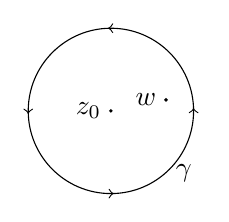
\begin{tikzpicture}[scale=0.7]
              \draw (0, 0) circle [radius=1.5];
              \fill (0, 0) circle (1pt) node[left] {$z_0$};
              \fill (1, 0.2) circle(1pt) node[left] {$w$};
              \draw[->] (1.5,-0.05) -- (1.5,0.05);
              \draw[->] (-1.5,0.05) -- (-1.5,-0.05);
              \draw[->] (0.05,1.5) -- (-0.05,1.5);
              \draw[->] (-0.05,-1.5) -- (0.05,-1.5);
              \node[below right] at (1,-0.8) {$\gamma$};
            \end{tikzpicture}\]
        Тогда, оказывается, (посчитаем чуть позже):
    \[\int\limits_{\gamma}\frac{\d z}{z - w} = \all{0,&|z - w| > r \\ 2\pi i,&|z - w| < r}\tag{$\circ$}\label{circle-integral}\]
    Грубой силой этот интеграл посчитать непросто, так как $w$ находится где угодно --- внутри или снаружи круга --- а интеграл, оказывается, зависит только от этих двух альтернатив.
    }
    \theorem[Основная оценка интеграла вдоль пути]{
        Пускай $\Phi = \sum\limits_{j=1}^n f_j\d x_j$ --- непрерывная дифференциальная форма в области $G \subset \R^n$, а $\gamma: [a, b] \map G$ --- кусочно-гладкий путь, $K \coloneqq \Image(\gamma) \subset G$.

    Тогда $\abs{\int\limits_{\gamma}\Phi} \le \underbrace{\sup\limits_{x \in K}\left(\sum\limits_{j = 1}^{n}|f_j(x)|^2\right)^{\nicefrac{1}{2}}}_{\eqqcolon A}\cdot l(\gamma)$.
    \provehere{
    Считаем, что $\gamma$ --- гладкий путь, иначе нужно разбить на кусочки гладкости.
    \[\abs{\int\limits_{\gamma}\Phi} = \abs{\int\limits_{a}^{b}\sum\limits_{j = 1}^{n}f_j\left(\gamma(t)\right)\gamma_j'(t)\d t} \underset{\text{КБШ}}\le \int\limits_{a}^{b}\left(\sum\limits_{j = 1}^{n}|f_j(\gamma(t))|^2\right)^{\nicefrac{1}{2}} \cdot \left(\sum\limits_{j = 1}^{n}|\gamma_j'(t)|^2\right)^{\nicefrac{1}{2}}\d t \le A \cdot \underbrace{\int\limits_{a}^{b}\left(\sum\limits_{j = 1}^{n}|\gamma_j'(t)|^2\right)^{\nicefrac{1}{2}}\d t}_{l(\gamma)}\]
    }
    }
    \newlection{1 марта 2024 г.}
    Рассмотрим дифференциальную форму $\Phi = F(z)\d z$, где $F$ --- непрерывная функция в $G \subset \C$.
    Пусть $\gamma: [a, b] \map G$ --- плоский путь.

    Расписав $\Phi(z) = F(z)\d x + i F(z)\d y$ и применив основную оценку интеграла вдоль пути, получаем
    \[\abs{\int\limits_{\gamma}\Phi} \le \max\limits_{z \in K}\sqrt{|F(z)|^2 + |F(z)|^2} \cdot l(\gamma) = \sqrt{2}\max\limits_{z \in K}|F(z)| \cdot l(\gamma)\]
    Эта оценка вызывает некоторую неудовлетворённость: кажется, что $\sqrt{2}$ здесь лишний.
    И это действительно правда: можно расписать интеграл аккуратнее.

    Пусть $\gamma = \gamma_1 + i\gamma_2$, тогда по определению
    \[\int\limits_{\gamma}\Phi = \int\limits_{a}^{b}F(\gamma(t))\cdot \gamma_1'(t) + i F(\gamma(t))\cdot \gamma_2'(t)\d t = \int\limits_{a}^{b}F(\gamma(t)) \cdot \gamma'(t)\d t\]
    Таким образом, интеграл от комплексной формы вдоль пути имеет более простое представление, и оно легко поддаётся более плотной оценке:
    \[\abs{\int\limits_{\gamma}\Phi} \le \int\limits_{a}^{b}|F(\gamma(t))| \cdot |\gamma'(t)|\d t \le \max\limits_{z \in K}|F(z)| \underbrace{\int\limits_{a}^{b}|\gamma'(t)|\d t}_{l(\gamma)}\]

    Посчитаем анонсированный на предыдущей лекции интеграл~\eqref{circle-integral}.
    Пусть $z_0, w \in \C$, $r > 0$.
    \bullets{
        \item Сначала рассмотрим случай $|w - z_0| < r$.
        Заметим, что, согласно основной оценке интеграла, если коэффициенты равномерно стремятся к какому-то значению и интегралы ограничены, то предельный интеграл тоже сходится.

        Запись ниже $\int\limits_{|z - z_0| = r}$, и вообще все аналогичные записи, которые встретятся в дальнейшем, по умолчанию означают, что граница соответствующего множества (в данном случае --- круга) обходится стандартным образом, то есть против часовой стрелки.
        \multline{\int\limits_{|z - z_0| = r}\frac{\d z}{z - z_0 - (w - z_0)} = \int\limits_{|z - z_0| = r}\frac{1}{z - z_0}\frac{1}{1 - \frac{w - z_0}{z - z_0}}\d z =\\= \int\limits_{|z - z_0| = r}\frac{1}{z - z_0}\left(1 + \frac{w - z_0}{z - z_0} + \left(\frac{w - z_0}{z - z_0}\right)^2 + \dots\right)\d z \circlesign{=}}
        На слагаемые из ряда имеется равномерная по $z$ оценка: $\abs{\frac{w - z_0}{z - z_0}} \le \frac{|w - z_0|}{r} < 1$, и по теореме Вейерштрасса функциональный ряд сходится.
        Значит, сумму можно вынести из-под интеграла
        \[\circlesign{=}\int\limits_{|z - z_0| = r}\frac{1}{z - z_0}\d z + \sum\limits_{j = 1}^{\infty}\ \int\limits_{|z - z_0| = r}\frac{(w - z_0)^j}{(z - z_0)^{j+1}}\d z \circlesign{=}\]
        Первое слагаемое мы умеем брать, а у каждого слагаемого из остальной суммы имеется первообразная: $\frac{1}{(z - z_0)^{j+1}} = -\frac{1}{j}\left(\frac{1}{(z - z_0)^{j}}\right)'$
        \[\circlesign{=}\int\limits_{|z - z_0| = r}\frac{1}{z - z_0}\d z = \int\limits_{0}^{2\pi}\frac{r i e^{it}}{r e^{it}}\d t = 2 \pi i\]
    \item Теперь разберёмся со случаем $|w - z_0| > r$.
        \[\int\limits_{|z - z_0| = r}\frac{\d z}{z - z_0 - (w - z_0)} = -\frac{1}{w - z_0}\int\limits_{|z - z_0| = r}\frac{\d z}{1 - \frac{z - z_0}{w - z_0}} = -\frac{1}{w - z_0}\sum\limits_{j = 0}^{\infty}\ \int\limits_{|z - z_0| = r}\frac{(z - z_0)^j}{(w - z_0)^j}\d z\]
    Аналогично предыдущему случаю, ряд сходится абсолютно, поэтому сумму опять можно вынести из под интеграла, и в данном случае всё ещё проще: каждое слагаемое имеет первообразную, там нет отрицательных степеней $z$, поэтому вся сумма обращается в нуль.
    }
    Пусть $\Phi = f_1 \d x_1 + \dots + f_n \d x_n$ --- непрерывная дифференциальная форма в некоторой области $G \subset \R^n$.
    \theorem{
    	\label{cross-partial}
    Если все функции $f_j \in C^1$, то следующие условия эквивалентны:
    \bullets{
    \item $\Phi$ замкнута.
    \item $\forall 1 \le i, j \le n: \der{f_i}{x_j} = \der{f_j}{x_i}$ --- <<накрест взятые частные производные равны>>.
    }
    \provenumbers{
    \item[$\then$] Выберем $x \in G$, так как форма замкнута, то $\exists U \ni x: \Phi$ имеет первообразную $F: U \map \R$.
    Тем самым, $f_i = \der{F}{x_i}$, и так как $f_i \in C^1$, то действительно $\der{f_j}{x_i} = \frac{\partial^2F}{\partial x_i \partial x_j} = \frac{\partial^2F}{\partial x_j \partial x_i} = \der{f_i}{x_j}$.
    \item[$\when$] Сначала приведём доказательство случая $n = 2$.
        В таком случае $\Phi = f\d x + g \d y$.

        Согласно посылке, $h \coloneqq \der{f}{y} = \der{g}{x}$.
        Кстати, равенство слева равносильно одному из эквивалентных уравнений Коши --- Римана.

        Рассмотрим произвольный $P = [a, b] \times [c, d] \subset G$, и докажем, что $\int\limits_{\partial P}\Phi = 0$.
        \[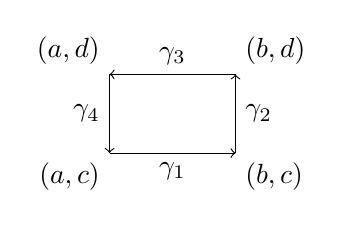
\begin{tikzpicture}
              \draw (0,0) node[below left] {$(a, c)$};
              \draw (0,1) node[above left] {$(a, d)$};
              \draw (1.6,0) node[below right] {$(b, c)$};
              \draw (1.6,1) node[above right] {$(b, d)$};

              \node at (0.8,0) [below] {$\gamma_1$};
              \node at (1.6,0.5) [right] {$\gamma_2$};
              \node at (0.8,1) [above] {$\gamma_3$};
              \node at (0,0.5) [left] {$\gamma_4$};

              \draw[->] (0,0) -- (1.6, 0);
              \draw[->] (1.6,0) -- (1.6, 1);
              \draw[->] (1.6,1) -- (0, 1);
              \draw[->] (0,1) -- (0, 0);
        \end{tikzpicture}\]
        То, что мы увидим сейчас, является первым заходом на \emph{формулу Остроградского --- Гаусса}.
        Функция $h$ непрерывна, и можно записать на неё интеграл Лебега:  $\int\limits_{P}h(x, y)\d x \d y$. % "записать на неё"?
        Теперь, применяя теорему Фубини, раскладываем интеграл в сумму повторных:
        \multline{\int\limits_{\gamma_3^-}f(\_, d)\d x + \int\limits_{\gamma_1^-}f(\_, c)\d x = \int\limits_{a}^{b}\left[f(x, d) - f(x, c)\right]\d x = \int\limits_{a}^{b}\left(\int\limits_{c}^{d}\der{f}{y}\d y\right)\d x
            =\\= \int\limits_{P}h(x, y)\d x \d y =\\=
            \int\limits_{c}^{d}\left(\int\limits_{a}^{b}\der{g}{x}\d x\right)\d y = \int\limits_{c}^{d}\left[g(b, y) - g(a, y)\right]\d y = \int\limits_{\gamma_2}g(b, \_)\d y + \int\limits_{\gamma_4}g(a, \_)\d y}
        Итого, $\int\limits_{\gamma_3^-}f(\_, d)\d x + \int\limits_{\gamma_1^-}f(\_, c)\d x = \int\limits_{\gamma_2}g(b, \_)\d y + \int\limits_{\gamma_4}g(a, \_)\d y$, откуда действительно $\int\limits_{\gamma}\Phi = 0$.
    \item[$\when$] Теперь приведём альтернативное доказательство индукцией по $n$.

    \underline{База:} Случай $n = 1$ тривиален: теорема Ньютона --- Лейбница говорит, что у непрерывной функции есть первообразная.

    \underline{Переход:} Пусть $n > 1$, и для $n - 1$ теорема доказана.
    Рассмотрим $a \in G$, и возьмём прямоугольный параллелепипед со сторонами, параллельными осям координат $P$ такой, что $a \in \Int P$.
        Докажем, что на $P$ у $\Phi$ есть первообразная.

    Построим $g(x_1, \dots, x_n) = \int\limits_{a_1}^{x_1}f_1(t, x_2, \dots, x_n)\d t$. Обозначим $\phi_j \coloneqq \der{g}{x_j}$.
        Заметим, что $\phi_1 = \der{g}{x_1} = f_1$.

    Теперь рассмотрим форму $\Psi(x_1, \dots, x_n) = \phi_1 \d x_1 + \dots + \phi_n \d x_n$.
        Эта форма имеет первообразную $g$ на параллелепипеде $P$.

    Теперь посмотрим на $\Phi - \Psi \eqqcolon h_1 \d x_1 + \dots + h_n \d x_n$.
        По построению $h_1 = 0$.
        По условию накрест взятые частные производные равны у $\Phi$, и они равны у $\Psi$, так как у неё есть первообразная.
    Значит, это же верно и для разности, в частности, $\der{h_i}{x_1} = \der{h_1}{x_i} = 0$.
        Иными словами, $\forall i: h_i$ не зависит от $x_1$.

    А раз так, то на $\Phi - \Psi$ можно смотреть, как на форму $(n-1)$-й переменной, и применить индукционное предположение.

    \note{
        Тут есть некоторый обман: производные $\der{\phi_i}{x_j}$ могут просто не существовать.

        Попробуем обойти его так: пусть $\beta \in C^\infty$, с компактным носителем.
        Выберем аппроксимативную единицу $\beta_t(x) = \frac{1}{t^n}\beta(\frac{x}{t})$.

        Назначим $f_k^{(t)} = f_k * \beta_t$, $f_k^{(t)} \underset{t \to 0}\rightrightarrows f_k$.

        Далее у формы $\Phi^{(t)}$ коэффициенты $h_k^{(t)}$ не зависят от $x_1$. А раз они равномерно стремятся к $h_k$, то и они не зависят от $x_1$.
        \comment{
        Это было произнесено устно, я наверняка что-то не так записал.
        }
        % Там было что-то про возьмём малый палраллелепипед и большой (и малое t) так, чтобы при вычислении свётки из малого параллелепипеда мы не выходили за большой, как-то так объясняли равномерную сходимость f_k^{(t)} на всём P. 
    }
    }
    }
    \theorem[Коши]{
    Пусть $F$ --- голоморфная функция в открытом множестве $G \subset \C$. Тогда дифференциальная форма $F(z)\d z$ замкнута, то есть локально $\exists S: S'(z) = F(z)$.
        \note{
        Теорема совсем проста, если заранее предположить, что $F'(z)$ непрерывна (а так в итоге и должно получиться, так как $F$ --- аналитична~(\cref{analytic-is-holomorphic})).
        В таком случае имеется следующее более простое доказательство.
        \provehere{
            Надо проверить второе уравнение Коши --- Римана: $\forall z \in \C: \der{F}{y}(z) = i \der{F}{x}(z)$ (первое выполнено, так как накрест-взятые частные производные равны).

            Поскольку $F(z)\d z = F(z)\d x + i F(z)\d y$, утверждение эквивалентно (согласно (\cref{cross-partial})) тому, что $\forall z \in \C: \der{F}{y}(z) = i \der{F}{x}(z)$.
        Пусть $F(z) = u(x, y) + i v(x, y)$.
        \[\der{u}{y} + i\der{v}{y} \underset{?}= i\left(\der{u}{x} + i\der{v}{x}\right)\]
        то есть $\der{u}{y} = -\der{v}{x}$ и $\der{v}{y} = \der{u}{x}$.
        \comment{Я вообще не понял, что произошло.}
        }
        }
        Теперь докажем теорему Коши вне предположения непрерывности производной.
    \provehere{
    Докажем от противного: пусть форма $F(z)\d z$ не замкнута, $\exists P_0 \subset G: \alpha = \int\limits_{\partial P_0}F(z)\d z \ne 0$.

    Будем потихонечку делить этот прямоугольник на четыре равные части: пусть $P_0 = Q_1 \cup Q_2 \cup Q_3 \cup Q_4$.
        \[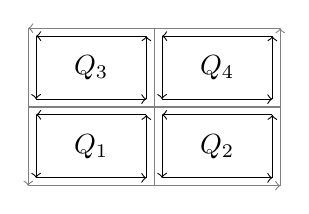
\begin{tikzpicture}
              \draw[->,color=gray] (0,0) -- (3.2, 0);
              \draw[->,color=gray] (3.2,0) -- (3.2, 2);
              \draw[->,color=gray] (3.2,2) -- (0, 2);
              \draw[->,color=gray] (0,2) -- (0, 0);
              \draw[color=gray] (0,1) -- (3.2,1);
              \draw[color=gray] (1.6,0) -- (1.6,2);
              \foreach \x/\y/\i in {0/0/1,1.6/0/2,0/1/3,1.6/1/4} {
                  \draw[->] ({\x+0.1},{\y+0.1}) -- ({\x+1.5}, {\y+0.1});
                  \draw[->] ({\x+1.5},{\y+0.1}) -- ({\x+1.5}, {\y+0.9});
                  \draw[->] ({\x+1.5},{\y+0.9}) -- ({\x+0.1}, {\y+0.9});
                  \draw[->] ({\x+0.1},{\y+0.9}) -- ({\x+0.1}, {\y+0.1});
                  \node at ({\x + 0.8}, {\y + 0.5}) {$Q_{\i}$};
              }
        \end{tikzpicture}\]
    Модуль интеграла по границе по крайней мере одного из $Q_i$ хотя бы $\frac{|\alpha|}{4}$.
        Назовём этот прямоугольник $P_1$, и продолжим процесс.
        Получим систему вложенных замкнутых прямоугольников $P_0 \supset P_1 \supset \dots$, таких, что $\abs{\int\limits_{\partial P_k}F(z)\d z} \ge \frac{|\alpha|}{4^k}$.
        При этом $l(\partial P_k) = 2^{-k}l(\partial P_0)$, и $\diam (P_k) = 2^{-k} \diam(P_0)$.

    Имеется ровно одна точка $z_0$ в пересечении $\bigcap\limits_{k \ge 0}P_k$.
        Воспользуемся условием того, что $F$ голоморфна в точке $z_0$: $F(z) = F(z_0) + F'(z_0)(z - z_0) + \underbrace{\psi(z)}_{o(|z - z_0|)}$

    Зафиксируем $\eps > 0$. $\exists \delta > 0: |z - z_0| < \delta \then |\psi(z)| \le \eps|z - z_0|$.
        Пусть $k$ настолько велико, что $\diam P_k < \delta$.
    \[\int\limits_{\partial P_k}F(z)\d z = \int\limits_{\partial P_k}[F(z_0) + F'(z_0)(z -z_0)]\d z + \int\limits_{\partial P_k}\psi(z)\d z\]
    Первый интеграл обнуляется, так как это линейная функция по $z$, у неё есть первообразная.
        Оценивая второй интеграл, получаем \[\frac{|\alpha|}{4^k} \le \abs{\int\limits_{\partial P_k}\psi(z)\d z} \le \eps\diam P_k \cdot l(\partial P_0) = \eps\cdot2^{-k}\diam P_0 \cdot 2^{-k}l(\partial P_0) = 4^{-k}\eps \cdot \diam P_0 \cdot l(\partial P_0)\]
    Выбирая довольно маленький $\eps$, получаем, что $|\alpha|$ меньше любого положительного числа.
    }
    }
    \theorem[Об устранимой особенности замкнутой дифференциальной формы]{\label{disposable-feature}
        Пускай $\Phi = f \d x + g\d y$ --- непрерывная дифференциальная форма в области $G \subset \C$.

        Если $z_0 \in G$, и $\Phi$ замкнута в $G \sm \{z_0\}$, то $\Phi$ замкнута в $G$.
        \provehere{
            Докажем, что $\forall P \subset G: \int\limits_{\partial P}\Phi = 0$.
            Рассмотрим случаи.
        \bullets{
            \item Если $z_0 \notin P$, то интеграл нуль по условию.
            \item Если $z_0 \in \Int P$, то данный случай сводится к следующему: разобьём прямоугольник на два так, чтобы $z_0$ оказалось на границе:
            \[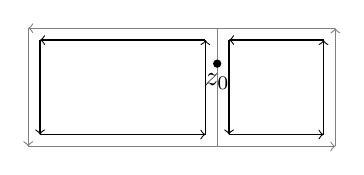
\begin{tikzpicture}[scale=1.5]
                  \draw[->,color=gray] (0,0) -- (2.6, 0);
                  \draw[->,color=gray] (2.6,0) -- (2.6, 1);
                  \draw[->,color=gray] (2.6,1) -- (0, 1);
                  \draw[->,color=gray] (0,1) -- (0, 0);
                  \draw[color=gray] (1.6,0) -- (1.6,1);
                  \fill (1.6,0.7) circle (1pt) node[below] {$z_0$};
                  \foreach \x/\w in {0/1.6, 1.6/1} {
                      \draw[->] ({\x+0.1},{0.1}) -- ({\x+\w-0.1}, {0.1});
                      \draw[->] ({\x+\w-0.1},{0.1}) -- ({\x+\w-0.1}, {0.9});
                      \draw[->] ({\x+\w-0.1},{0.9}) -- ({\x+0.1}, {0.9});
                      \draw[->] ({\x+0.1},{0.9}) -- ({\x+0.1}, {0.1});
                  }
            \end{tikzpicture}\]
            \item Если $z_0 \in \partial P$, то отступим на $\eps$, интеграл по границе $P_\eps$ будет нулём: $\int\limits_{\partial P_\eps}\Phi = 0$. % Без картинки непонятно, что за $P_\eps$

        Заметим, что $\int\limits_{\partial P_\eps}\Phi \underset{\eps \to 0}\Map \int\limits_{\partial P}\Phi$, так как коэффициенты дифференциальной формы равномерно непрерывны в некоторой окрестности $P$.
            Значит, $\int\limits_{\partial P}\Phi = 0$. % Тут чего-то надо расписать про то, что две стороны сокращаются, а другие две стороны просто короткие, длины \eps
        }
        }
    }
    \theorem[Малая интегральная формула Коши]{\label{integral-form}
    Пусть $f$ --- голоморфна в области $G$, $B = B(z_0, r)$ --- круг, $\overline{B} \subset G$. Тогда $\forall z \in B$:
    \[f(z) = \frac{1}{2\pi i}\int\limits_{\partial B}\frac{f(\zeta)}{\zeta - z}\d \zeta\]
    \provehere{
    Докажем для некоего фиксированного $z \in B$.

        Рассмотрим функцию $g(\zeta) = \frac{f(z) - f(\zeta)}{z - \zeta}$.
        $g$ голоморфна в области $G \sm \{z\}$. Тем самым, $g(\zeta)\d \zeta$ --- замкнутая форма в $G \sm \{z\}$, а по теореме об устранимой особенности $g(\zeta)\d \zeta$ замкнута в $G$ (доопределим по непрерывности $g(z) \coloneqq f'(z)$).

        Но так как круг --- удобная область, то у $g$ имеется первообразная в некотором круге $B(z_0, r(1 + \eps))$ (где $\eps > 0$ настолько мал, что $B(z_0, r(1 + \eps)) \subset G$),

        Тем самым, $\int\limits_{|\zeta - z_0| = r}\frac{f(z) - f(\zeta)}{z - \zeta}\d \zeta = 0$, откуда \[\int\limits_{|\zeta - z_0| = r}\frac{f(\zeta)}{\zeta - z}\d \zeta = \int\limits_{|\zeta - z_0| = r}\frac{f(z)}{\zeta - z}\d \zeta = f(z)\cdot\int\limits_{|\zeta - z_0| = r}\frac{1}{\zeta - z}\d \zeta = 2\pi i \cdot f(z)\]
    }
    }
    \corollary[Теорема Коши]{\label{holomorphic-then-analytic}
    Если функция голоморфна в области $G \subset \C$, то $\forall z_0 \in G$ функция $f$ (в некоторой окрестности) раскладывается в некоторый степенной ряд $f(z) = \sum\limits_{n = 0}^{\infty}c_n(z - z_0)^n$, причём радиус сходимости хотя бы $\dist(z_0, \partial G)$.
    \provehere{
        Пусть $r \in (0, \dist(z_0, \partial G))$.
        Рассмотрим $B = B_r(z_0)$. Так как $B \subset G$, то для точки $z \in B$ получаем
    \multline{f(z) = 
    	\frac{1}{2\pi i}\int\limits_{|\zeta - z_0| = r}\frac{f(\zeta)}{\zeta - z}\d \zeta =
    	\frac{1}{2\pi i}\int\limits_{|\zeta - z_0| = r}\frac{f(\zeta)}{(\zeta - z_0) - (z - z_0)}\d \zeta =
    	\\
    	= \frac{1}{2\pi i}\int\limits_{|\zeta - z_0| = r}\frac{1}{\zeta - z_0}\cdot \frac{1}{1 - \frac{z - z_0}{\zeta - z_0}}f(\zeta)\d\zeta =
    	\frac{1}{2\pi i}\sum\limits_{j = 0}^{\infty}(z - z_0)^{j}\int\limits_{|\zeta - z_0| = r}\frac{f(\zeta)}{(\zeta - z_0)^{j+1}}\d \zeta}
        Абсолютная равномерная сходимость в круге радиус $r$ при $r < \dist(z_0, \partial G)$ имеется по тем же причинам, что и при доказательстве~\eqref{circle-integral}.

        Таким образом, мы получили степенной ряд, и так как коэффициенты степенного ряда, раз определены, не зависят от радиуса круга ($c_j = \frac{f^{(j)}(z_0)}{j!}$), то радиус сходимости данного ряда хотя бы $\dist(z_0, \partial G)$.
    }
    }
    \newlection{12 марта 2024 г.}
    \note{
        Интегральную форму Коши можно спокойно дифференцировать: так,
    \[\frac{\d}{\d z}f(z) = \frac{\d}{\d z}\left(\frac{1}{2\pi i}\int\limits_{|\zeta - z_0| = r}\frac{f(\zeta)}{\zeta - z}\d\zeta\right) = \frac{1}{2\pi i}\int\limits_{|\zeta - z_0| = r}\frac{f(\zeta)}{(\zeta - z_0)^2}\d\zeta\]
    В общем случае
        \[\frac{\d^k}{\d z^k}f(z) = \frac{\d^k}{\d z^k}\left(\frac{1}{2\pi i}\int\limits_{|\zeta - z_0| = r}\frac{f(\zeta)}{\zeta - z}\d\zeta\right) = \frac{k!}{2\pi i}\int\limits_{|\zeta - z_0| = r}\frac{f(\zeta)}{(\zeta - z_0)^{k+1}}\d\zeta\]
    }
    \definition[Целая (entire) функция]{
        Голоморфная функция, заданная в $\C$.
    }
    Выберем $z_0 = 0$.
    Согласно~(\cref{holomorphic-then-analytic}), получаем $f(z) = \sum\limits_{j = 0}^{\infty}c_j$, где $c_j = \frac{1}{2\pi i}\int\limits_{|\zeta| = r}\frac{f(\zeta)}{\zeta^{j+1}}\d\zeta$, причём имеется абсолютная сходимость везде в $\C$.
    \theorem{
    Если $f$ целая, и $|f(z)| = \bigO(z^N)$ при $|z| \underset{z \to \infty}\Map \infty$, то $f$ --- многочлен степени не более $N$.
    \provehere{
        Из определения $\bigO: \exists C, a \in \R: |f(z)| \le C|z|^N$ при $|z| > a$.

        Выберем $r > a$, и оценим: $|c_j| = \abs{\frac{1}{2\pi i}\int\limits_{0}^{2\pi}\frac{f\left(r e^{i\theta}\right)}{(re^{i\theta})^{j+1}}i re^{i\theta}\d\theta} \le \frac{1}{2\pi}\int\limits_{0}^{2\pi}\frac{C r^N}{r^j}\d\theta = \frac{C r^N}{r^j}$.
        Получается, при $j > N: |c_j|$ меньше любого наперёд заданного положительного числа.
    }
    }
    \corollary[Теорема Лиувилля]{
        Ограниченная целая функция постоянна.
    }
    \corollary[Основная теорема алгебры]{
        $\forall p \in \C[z]: \deg p > 0 \then \exists z_0 \in \C: p(z_0) = 0$.
    \provehere{
        Пусть $p(z) = \sum\limits_{j = 0}^{N}c_j z^j$, где $N > 0$ и $c_N \ne 0$.

    Пойдём от противного: пусть $\forall z \in \C: p(z) \ne 0$.

    Рассмотрим $f(z) \coloneqq \frac{1}{p(z)}$.
        \bullets{
            \item С одной стороны, это целая функция: $\frac{\d}{\d z}f(z) = -\frac{p'(z)}{p(z)^2}$.

        \item С другой стороны, $f$ ограничена:
        оценим $|p(z)| \ge |z^N|\left(|c_N| - \sum\limits_{j = 0}^{N - 1}\frac{|c_j|}{|z|^{N-j}}\right)$, откуда для достаточно больших $|z|: |p(z)| \ge \frac{|c_N|}{2}|z|^N$.

        Тем самым, $p(z) \underset{|z| \to \infty}\Map \infty$, то есть $f(z) \underset{|z| \to \infty}\Map 0$.
            А при малых $|z|: f$ ограничена, как непрерывная функция на компакте.
        \item Тем самым, по теореме Лиувилля, $f \equiv \const$, то есть $p \equiv \const$. Противоречие, мы предполагали $\deg p > 0$.\qedhere
        }
    }
    }
    \theorem[Теорема о среднем]{
    Пусть $z_0 \in G, f: G \map \C$ голоморфна в $G$.
        Выберем $r < \dist(z_0, \partial G)$.
        Тогда \encircle{f(z_0) = \frac{1}{2\pi}\int\limits_{0}^{2\pi}f(z_0 + r e^{it})\d t}
        \provehere{
            Посчитаем $f(z_0)$ по интегральной формуле:
            \[f(z_0) = \frac{1}{2\pi i}\int\limits_{|\zeta - z_0| = r}\frac{f(\zeta)}{\zeta - z_0}\d\zeta = \frac{1}{2\pi i}\int\limits_{0}^{2\pi}\frac{f(z_0 + r e^{it})i r e^{it}}{r e^{it}}\d t = \frac{1}{2\pi}\int\limits_{0}^{2\pi}f(z_0 + r e^{it})\d t\]
        }
    }
    Это действительно среднее в обычном смысле: $f$ проинтегрирована по окружности по мере Лебега, и интеграл поделили на меру окружности.
    \theorem[Принцип максимума модуля]{\label{maximum-on-boundary}
        Пусть $f: G \map \C$ --- непостоянная голоморфная функция. Тогда $|f|: z \mapsto |f(z)|$ не может достигать наибольшего значения при $z \in G$.
        \provehere{
            Пойдём от противного: пусть $\exists z_0 \in G: \forall z \in G: |f(z)| \le |f(z_0)|$.
            Выберем $r > 0: B(z_0, r) \subset G$, и докажем, что $|f|$ постоянна в $B(z_0, r)$.
            Пусть $\rho < r$, по теореме о среднем $|f(z_0)| = \frac{1}{2\pi}\abs{\int\limits_{0}^{2\pi}f(z_0 + \rho e^{it})\d t} \le \frac{1}{2\pi}\int\limits_{0}^{2\pi}\underbrace{|f(z_0 + \rho e^{it})|}_{\le |f(z_0)|}\d t$, причём равенство достигается только если $\forall t \in [0, 2\pi]: |f(z_0 + \rho e^{it})| = |f(z_0)|$ (если $\exists t_0 \in (0, 2\pi): |f(z_0 + \rho e^{it_0}| < |f(z_0)|)$, то по непрерывности $\exists \eps > 0: \forall t \in (t_0 - \eps, t_0 + \eps): |f(z_0 + \rho e^{it}| < |f(z_0)| - \eps$, то есть на промежутке $(t_0 - \eps, t_0 + \eps)$ интеграл строго меньше требуемого значения).
            \indentlemma{
                Пусть $f: G \map \C$ голоморфна, и $\exists z_0 \in G: f'(z_0) \ne 0$. Тогда $\exists U \ni z_0: f(z_0) \in \Int f(U)$.
            }{
                Теорема об обратной функции.
            }
            Тем самым, $\forall z \in B(z_0, r): f'(z) = 0$ (так как $|f(z)|$ --- максимум).

        Далее применяем теорему единственности, доказанную во II семестре: $f$ и константа, равная $|f(z_0)|$ совпадают на множестве с предельной точкой, значит, они совпадают везде в $G$.
        }
    }
    \corollary{
    Пусть $G$ --- ограниченная область, $f: \overline{G} \map \C$ голоморфна в $G$. Тогда $\forall z \in G: |f(z)| \le \max\limits_{\zeta \in \partial G}|f(\zeta)|$.
    \provehere{
    $f$ достигает своё наибольшее значение на компакте $\overline{G}$, но согласно принципу максимума, это значение достигается не внутри $G$.
    }
    }
    \section{Гармонические функции}
    Запишем теорему о среднем для $f: G \map \C$:
    \[f(z_0) = \int\limits_{1}{2\pi}(f(z_0) + r e^{it})\d t\]
    Пусть $f = u + iv$, где $u, v$ --- вещественные функции в $G$.
    Теорема о среднем говорит, что
    \[u(z_0) = \int\limits_{1}{2\pi}(u(z_0) + r e^{it})\d t \qquad v(z_0) = \int\limits_{1}{2\pi}(v(z_0) + r e^{it})\d t\]
    Так как $f$ аналитична, то в вещественном смысле $u, v \in C^{\infty}(G)$.

    Запишем уравнения Коши --- Римана:
    \[\der{u}{x} = \der{v}{y} \quad \der{u}{y} = -\der{v}{x}\]
    Дифференцируя второй раз, получаем \[\all{\frac{\partial^2 u}{\partial x^2} = \frac{\partial^2 v}{\partial x \partial y} \\ \frac{\partial^2 u}{\partial y^2} = -\frac{\partial^2 v}{\partial x \partial y}}\]
    Это так называемое \emph{уравнение Лапласа}: $\frac{\partial^2 u}{\partial x^2} + \frac{\partial^2 u}{\partial y^2} = 0$.

    Обобщим.
    Пусть $G \subset \R^n$ --- область, пусть $f \in C^2(G)$.
    \definition[$f$ --- гармоническая функция в $G$]{
        $\frac{\partial^2u}{\partial x_1^2} + \cdots + \frac{\partial^2u}{\partial x_n^2} = 0$.
    }
    Оператор $\Delta = \frac{\partial^2}{\partial x_1^2} + \cdots + \frac{\partial^2}{\partial x_n^2}$ называется \emph{оператором Лапласа}, и понятно, что гармонические функции --- в точности такие $u$, что $\Delta u = 0$.
    \statement{
    Если $u \in C^2(G)$, где область $G \subset \R^2$, то локально существует голоморфная $f: u = \Re f$.
        Иными словами, $\forall z_0 \in G: \exists U \ni z_0, \exists$ аналитическая $f: U \map \C: u = \Re f$.
    \provehere{
        Пусть $\phi \coloneqq \der{u}{x}, \psi \coloneqq -\der{u}{y}$. Тогда $\der{\phi}{x} - \der{\psi}{y} = 0$, то есть $\der{\phi}{x} = \der{\psi}{y}$ везде в $G$.

    Раз накрест-взятые частные производные совпадают, то дифференциальная форма $\phi \d x + \psi \d y$ замкнута, значит, локально имеется первообразная.

    Зафиксируем точку $z_0 \in G$, имеется некоторый шарик $B \ni z_0$, в котором есть первообразная $v$:
    \[\der{v}{x} = \psi = -\der{u}{y} \qquad \der{v}{y} = \phi = \der{u}{x}\]
    Это уравнения Коши --- Римана, значит, $f \coloneqq u + iv$ голоморфна в $B$.
    }
    }
    \theorem[Морера]{\label{morera}
        Пусть $f: (G \subset \C) \map \C$ непрерывна.
        Следующие условия эквивалентны.
        \numbers{
        \item $f$ голоморфна в $G$.
        \item $f$ аналитична в $G$.
        \item Дифференциальная форма $f(z)\d z$ замкнута.
        }
    \provehere{
        $(1) \iff (2)$ уже доказано:~(\cref{analytic-is-holomorphic}) и~(\cref{holomorphic-then-analytic}).

    $(1) \then (3)$ доказано тоже:~(\cref{cauchey-theorem}).

    Докажем $(3) \then (2)$.
        Пусть $F$ --- первообразная формы $f(z)\d z$ в круге $B(z_0, r) \subset G$.
        $F$ голоморфна в $B(z_0, r)$, и $\forall z \in D: F'(z) = f(z)$.

    Значит, $F$ раскладывается в степенной ряд $F(z) = \sum\limits_{j = 0}^{\infty}a_j (z - z_0)^j$. Отсюда ${f(z) = \sum\limits_{j = 1}^{\infty}j a_j (z - z_0)^{j - 1}}$.
    }}
    \section{Первообразная от замкнутой формы вдоль непрерывного пути}
    \subsection{Наводящие предположения}
    Пусть $f\d x + g\d y$ --- непрерывная дифференциальная форма в $G$, предположим, что она точная: имеется первообразная $F$.

    Пусть $\gamma: [a, b] \map G$ --- кусочно-гладкий путь.
    Ранее было получено, что $\int\limits_{\gamma}f \d x + g \d y = F(\gamma(b)) - F(\gamma(a))$.

    Давайте обобщим интеграл вдоль пути: пусть $\gamma: [a, b] \map G$ --- произвольный непрерывный путь.
    Положим по определению $\int\limits_{\gamma}f \d x + g \d y \bydef F(\gamma(b)) - F(\gamma(a))$.

    Теперь пусть $f\d x + g\d y$ всего лишь замкнута.
    Выберем $a = t_0 < t_1 < \cdots < t_k = b$ так, что $\forall j: \gamma([t_j, t_{j+1}])$ лежит в области $G_j$, в которой у формы $f\d x + g\d y$ есть первообразная $F_j$.
    Попробуем определить
    \[\int\limits_{\gamma\big|_{[t_j, t_{j+1}]}}f \d x + g \d y \bydef F_j(\gamma(t_{j + 1})) - F_j(\gamma(t_j))\]
    и
    \[\int\limits_{\gamma}f \d x + g \d y \bydef \sum\limits_{j = 0}^{k - 1}F_j(\gamma(t_{j + 1})) - F_j(\gamma(t_j))\]
    Проблема в том, чтобы доказать, что определение корректно --- не зависит от выбора разбиения $a = t_0 < \dots < t_k = b$.
    \subsection{Требуемые свойства}
    Пусть $\Phi = f \d x + g \d y$ --- замкнутая форма в области $G \subset \C$, и $\gamma: [a, b] \map G$ --- путь.

    \definition[Первообразная формы $\Phi$ вдоль пути $\gamma$]{
    Такая функция $v: [a, b] \map G$:
    \bullets{
    \item $\forall t \in [a, b]: \exists U \ni \gamma(t), \eps > 0$ и найдётся первообразная $F$ для $\Phi$ на $U$, такая, что \[\forall \tau \in (t - \eps, t + \eps): v(\tau) = F(\gamma(\tau))\]
    }
    }
    \fact{
    Функция $v$, если существует, непрерывна на $[a, b]$.
    \provehere{
        Непрерывность в какой-то конкретной точке следует из непрерывности композиции $F \circ \gamma$.
    }
    }
    \theorem{\label{antiderivative-along-path}
    Первообразная замкнутой дифференциальной формы вдоль пути $\gamma$ всегда существует, и любые две отличаются на константу.
    \provehere{
    Сначала докажем существование. Для всех $t \in [a, b]$ выберем окрестность $U_t \coloneqq B(\gamma(t), r_t)$, где $r_t$ настолько мал, что в $U_t$ есть первообразная.

    Семейство $\{U_t\}_{t \in [a, b]}$ образуют открытое покрытие $\gamma([a, b])$.
        По лемме Лебега $\exists \eps > 0: \forall t \in [a, b]: B(\gamma(t), \eps)$ содержится в каком-то $U_{t'}$.
        Применяя теорему Кантора о ранвомерной непрерывности, получаем существование разбиения $a = t_0 < \dots < t_k = b$, такое, что $\gamma([t_j, t_{j + 1}])$ лежит в одном из $U_t$.

        Произвольно выберем $v(a)$.
        Построим $v\big|_{[t_j, t_{j+1}]}$ индукцией по $j$.

        \underline{База:} Пусть $\gamma([t_0, t_1]) \subset U_0$, и имеется первообразная $F_0$ на $U_0$. Определим $v(\tau) = F_0(\gamma(\tau))$ при $\tau \in [t_0, t_1]$.

        \underline{Переход:} Пусть $\gamma([t_j, t_{j+1}]) \subset U_j, F_j$ --- первообразная $\Phi$ на $U_j$.
        Найдётся такое $\delta > 0: \gamma([t_j - \delta, t_{j+1}]) \subset U_j$, значит, $U_j \cap U_{j-1} \ne \o$.
        Это пересечение связно, на нём имеются две первообразные, $F_{j-1}$ и $F_j$.

        Добавим константу к $F_j$ так, чтобы $F_j \equiv F_{j-1}$ при $t \in [t_j - \delta, t_j]$, и определим $v(\tau) = F_j(\gamma(\tau))$ при $\tau \in [t_j, t_{j+1}]$.
        Окрестность $U_j$ захватывает отрезок $[t_j - \delta, t_{j+1}]$, значит, для точек во внутренности выполнено условие из определения первообразной.

        Докажем единственность: рассмотрим точку $t \in [a, b]$. Найдутся два круга $U, V \ni \gamma(t)$, и первообразные $F, H$ формы $\Phi$ в этих окрестностях, такие, что $u(\tau) = F(\gamma(\tau))$ и $v(\tau) = H(\gamma(\tau))$ при $\tau$, достаточно близких к $t$.

    Тем самым, $u - v$ локально постоянна, но локально постоянная функция на связном множестве --- константа (прообраз любого элемента из образа открыто-замкнут).
    }
    }
    \newlection{15 марта 2024 г.}
    Теперь определим интеграл $\int\limits_{\gamma}\Phi = v(b) - v(a)$, где $v$ --- первообразная для $\Phi$ вдоль пути $\gamma$, получившаяся из~(\cref{antiderivative-along-path}).
    Теперь интеграл определён для любой замкнутой формы вдоль пути (однако для кусочно-гладкого пути интеграл~(\cref{piecewise-smooth-integral}) был определён для необязательно замкнутой формы).
    \properties[Свойства первообразной вдоль пути]{
    \item Аддитивность по дифференциальной форме: $\int\limits_{\gamma}(\Phi + \Psi) = \int\limits_{\gamma}\Phi + \int\limits_{\gamma}\Psi$.
    \item Аддитивность вдоль пути: $\int\limits_{\gamma_1 \oplus \gamma_2}\Phi = \int\limits_{\gamma_1}\Phi + \int\limits_{\gamma_2}\Phi$.
    \item Если $\gamma$ --- кусочно-гладкий путь, то определение совпадает со старым.
    \provehere{
    $\gamma'$ существует везде, кроме, может быть, конечного множества.

    При помощи леммы Лебега разобьём отрезок точками $a = t_0 < \dots < t_k = b$ так, что $\forall j < k: \exists U_j \supset \gamma([t_j, t_{j+1}])$ такая, что на $U_j$ найдётся первообразная $H_j$:
    \[\forall \tau \in [t_j, t_{j+1}]: F(\tau) = H_j(\gamma(\tau))\]
    И старый, и новый интегралы аддитивны вдоль пути. Несложно видеть, что в обеих определениях $\int\limits_{\gamma\big|_{[t_j, t_{j+1}]}}\Phi$ совпадают.
    }
    \item Так как путь $\gamma$ необязательно дифференцируем, то основную оценку интеграла вдоль пути распространить на новое определение проблематично: длины может не существовать.
    \item Пусть $\phi: [a, b] \map [c, d]$ --- гомеоморфизм, $\gamma: [a, b] \map G$ --- путь, тогда
    \[\int\limits_{\gamma}\Phi = \pm\int\limits_{\gamma \circ \phi}\Phi\]
    где знак зависит от того, возрастает $\phi$, или убывает.
    \provehere[Причина]{ Если $F$ --- первообразная $\Phi$ вдоль пути $\gamma$, то $F \circ \phi$ --- первообразная для $\Phi$ вдоль пути $\gamma \circ \phi$.
    }
    }
    \subsection{О гомотопности путей}
    Пусть $K = [0, 1] \times [a, b]$ --- квадрат гомотопии.
    \definition[Гомотопия]{Непрерывное отображение $\Gamma: K \map \C$.}
    Положим $\gamma_s \coloneqq \Gamma(s, \_)$.
    Как водится, $\gamma_0, \gamma_1$ --- два пути $[a, b] \map \C$, и существование $\Gamma$ по определению влечёт гомотопность этих путей.

    Пути $\gamma_0, \gamma_1: [a, b] \map G$ \emph{гомотопны в $G$}, если найдётся гомотопия $\Gamma: K \map G$.

    Будем говорить о гомотопности двух замкнутых путей $\gamma_1$ и $\gamma_2$ при условии существования гомотопии $\Gamma: K \map G$, соединяющей $\gamma_1$ и $\gamma_2$ в классе замкнутых путей: $\forall s \in [0, 1]: \Gamma(s, a) = \Gamma(s, b)$.

    Гомотопность путей --- отношение эквивалентности, также как и гомотопность замкнутых путей.

%    \theorem{
%        Пусть $F$ --- аналитическая функция в области $G$, а $\gamma_0$ и $\gamma_1$ --- замкнутые пути, гомотопные в $G$ (в классе замкнутых путей).
%    Тогда $\int\limits_{\gamma_1}F \d z = \int\limits_{\gamma_2}F \d z$.
%    \provehere{
%
%    }
%    }
%
    \definition[Односвязная область]{
        Область, в которой всякий замкнутый путь гомотопен постоянному.
        Иными словами, фундаментальная группа тривиальна.
    }
    \definition[Звёздная область $A \subset \R^n$]{
    Такая область, что для некоторого \emph{центра} $z_0 \in A$: $\forall z \in A: \defset{z_0 + s(z -z_0)}{s \in [0, 1]} \subset A$.
    }
    \[\begin{tikzpicture}
          \draw[dashed] (0.9, 0.5) -- (1, 2);
          \draw[dashed] (1, 2) -- (-0.2, 1);
          \draw[dashed] (-0.2, 1) -- (-2, 2);
          \draw[dashed] (-2, 2) -- (-1, 0.08);
          \draw[dashed] (-1, 0.08) -- (-2, -1);
          \draw[dashed] (-2, -1) -- (-0.4, -0.9);
          \draw[dashed] (-0.4, -0.9) -- (0.6, -2);
          \draw[dashed] (0.6, -2) -- (0.8, -0.7);
          \draw[dashed] (0.8, -0.7) -- (2, -0.2);
          \draw[dashed] (2, -0.2) -- (0.9, 0.5);
          \fill (0, 0) circle (1pt) node[right] {$z_0$};
          \fill (-1, 1) circle (1pt) node[right] {$z$};
          \draw[->] (0, 0) -- (-1, 1);
    \end{tikzpicture}\]
    \fact{Всякая звёздная область $A$ односвязна.
    \provehere{
    Прогомотопируем путь $\gamma: [a, b] \map A$ при помощи \begin{align*}\Gamma: [0, 1] \times [a, b] &\map K\\\tau, t &\mapsto z_0 \tau + (1 - \tau)\gamma(t)\qedhere\end{align*}
    }
    }
    \example[Неодносвязная область]{
    Пусть $A$ --- звёздная область, выкинем точку $w_0 \in A$.
        \[\begin{tikzpicture}
              \draw[dashed] (0.9, 0.5) -- (1, 2);
              \draw[dashed] (1, 2) -- (-0.2, 1);
              \draw[dashed] (-0.2, 1) -- (-2, 2);
              \draw[dashed] (-2, 2) -- (-1, 0.08);
              \draw[dashed] (-1, 0.08) -- (-2, -1);
              \draw[dashed] (-2, -1) -- (-0.4, -0.9);
              \draw[dashed] (-0.4, -0.9) -- (0.6, -2);
              \draw[dashed] (0.6, -2) -- (0.8, -0.7);
              \draw[dashed] (0.8, -0.7) -- (2, -0.2);
              \draw[dashed] (2, -0.2) -- (0.9, 0.5);
              \fill (0.5, 0.1) circle (1pt) node[right] {$w_0$};
              \draw (0.5, 0.1) circle (0.5);
              \draw[->] (0.45, 0.6) -- (0.55,0.6);
              \node[above] at (0.5, 0.6) {$\omega$};
        \end{tikzpicture}\]
    Интеграл $\frac{\d z}{z - w_0}$ по маленькой окружности $\omega$, обходящей $w_0$, равен $2\pi i$, значит, путь не стягиваем.
    }
    \theorem[Первообразная вдоль гомотопии]{
    Пусть $K = [0, 1] \times [a, b]$ --- квадрат, $\Gamma: K \map G$ --- гомотопия, и $\Phi = f \d x + g \d y$ --- замкнутая дифференциальная форма в $G$.
    Тогда $\exists F: K \map\C$ --- \emph{первообразная формы $\Phi$ вдоль гомотопии $\Gamma$}, то есть такая функция, что
    $\forall (s, t) \in K: \exists U \ni (s, t): U \subset G, \exists \delta > 0: \exists \Phi: U \map \C$ --- первообразная формы $F$, такая, что \[\all{|\sigma - s| < \delta \\ |\tau - t| < \delta} \then F(\sigma, \tau) = H(\Gamma(\sigma, \tau))\]
    \provehere{
    Покроем множество $\Gamma(K)$ кругами $U \subset G$, такими что в каждом круге $U$ у $\Phi$ есть первообразная $H_U$.

    По лемме Лебега $\exists \rho > 0: \forall e \subset K: \diam (e) < \rho \then e$ лежит в одном из кругов данного покрытия.

    Разобьём квадрат гомотопии $K$ на прямоугольники диаметра меньше $\rho$:
    \[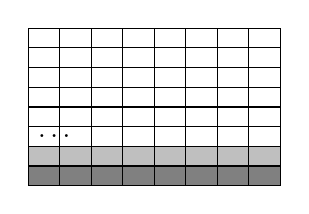
\begin{tikzpicture}
          \fill[gray] (0,0) rectangle (3.2, 0.25);
          \fill[lightgray] (0,0.25) rectangle (3.2, 0.5);
        \foreach \x in {0, 0.4, ..., 3.2} {
            \draw (\x, 0) -- (\x, 2);
        }
        \foreach \y in {0, 0.25, ..., 2} {
            \draw (0, \y) -- (3.2, \y);
        }
          \node[right] at (0, 0.625) {$\dots$};
    \end{tikzpicture}\]
    Аналогично доказательству~(\cref{integral-along-path}), в каждом горизонтальном прямоугольнике найдётся первообразная $F_j$, а дальше их надо сшить.
    Сшить несложно: вдоль горизонтального отрезка --- пересечения прямоугольничков --- $F_j\big|_{\dots} = F_{j+1}\big|_{\dots}$.
        Так как это --- первообразные вдоль пути, то они отличаются на константу. Значит, можно изменить все $F_j$ на константы так, чтобы их склейка была непрерывной функцией.

    Дальше надо проверить, что действительно получилась первообразная на квадрате.
        Выберем точку $(s, t) \in K$.
        Если точка попала внутрь какого-то прямоугольничка, то можно выбрать окрестность, лежащую внутри прямоугольничка, иначе чуть сложнее, но несильно.
    }
    }
    \theorem{
    Интегралы от замкнутой формы $\Phi$ по гомотопным замкнутым путям равны.
    \provehere{
    Определим $w(t) \coloneqq \int\limits_{\gamma_t}\Phi$ для всех $t \in [0, 1]$.

    Пусть $F$ --- первообразная для формы $\Phi$ вдоль гомотопии $\Gamma$. Понятно, что $w(t) = F(t, b) - F(t, a)$.

    Докажем, что $w$ локально постоянна на $[0, 1]$, следствием будет, что $w$ постоянна, что и требуется доказать.

    $\forall (\alpha, \beta) \in [0, 1] \times [a, b]$: $\exists \delta > 0$,  круг $U$ и первообразная $H_U$, такие, что
        \[\all{|\alpha - \alpha'| < \delta \\ |\beta - \beta'| < \delta} \then F(\alpha', \beta') = H_U(\Gamma(\alpha', \beta'))\]
    Пусть $U_1, U_2$ --- такие шары для $(t, b)$ и $(t, a)$ соответственно. \
    Тогда для $\tau$, достаточно близких к $t$, выполнено $w(t) = H_{U_1}(\Gamma(t, b)) - H_{U_2}(\Gamma(t, a))$.
    $H_1, H_2$ --- две первообразные в одной окрестности, они отличаются на константу, а $\Gamma(t, a) \equiv \Gamma(t, b)$, поэтому $w$ локально постоянна.
    }
    }
    \note{
    Если очень хочется, то можно соединить пути $\gamma_0: [a_0, b_0] \map \C$ и $\gamma_1: [a_1, b_1] \map \C$ гомотопией $\Gamma: K \map \C$, где $K \coloneqq \defset{(t, s)}{t \in [0, 1], s \in [a_t, b_t]}$ ($a_t, b_t$ --- какие-то непрерывные функции от $t$, такие, что $a_t < b_t$).
    }
    \section{Ряды Лорана}
    \emph{Ряд Лорана} $f(z)$ --- ряд вида $f(z) = \sum\limits_{n \in \Z}c_n (z - z_0)^n$.

    Говорят, что ряд Лорана сходится в точке $z$, если оба ряда $f_+(z) = \sum\limits_{n \ge 0}c_n (z - z_0)^n$ и $f_-(z) = \sum\limits_{n < 0}c_n (z - z_0)^n$ сходятся.

    Первый ряд степенной, имеется некий радиус сходимости $r_+$, такой, что $|z - z_0| < r_+ \then f_+$ сходится.
    При замене переменной $w \coloneq \frac{1}{z - z_0}$, $f_-(\nicefrac{1}{w})$ становится степенным рядом от $w$, сходящимся при $w < \frac{1}{r_-}$.

    Таким образом, ряд сходится абсолютно внутри <<кольца>> $\defset{z \in \C}{r_- < |z - z_0| < r_+}$:
    \[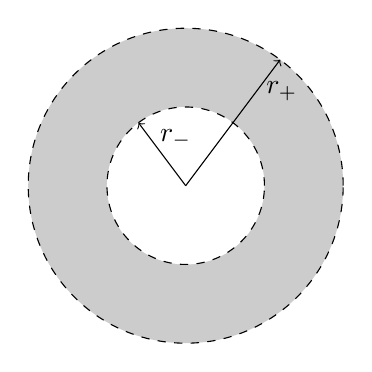
\begin{tikzpicture}
          \definecolor{lightgray}{rgb}{0.8,0.8,0.8}
          \fill[lightgray] (0, 0) circle (2);
          \fill[white] (0, 0) circle (1);
          \draw[->] (0, 0) -- (-0.6, 0.8) node[near end, right]{$r_-$};
          \draw[->] (0, 0) -- (1.2, 1.6) node[near end, right]{$r_+$};
          \draw[dashed] (0, 0) circle (2);
          \draw[dashed] (0, 0) circle (1);
    \end{tikzpicture}\]
    \theorem{
    Пусть $0 \le r_- < r_+ \le \infty$, функция $f$ голоморфна в <<кольце>> $K \coloneqq \defset{z \in \C}{r_- < |z| < r_+}$.

    Тогда $f$ представима в $K$ сходящимся рядом Лорана.
    \provehere{
    Пусть $z \in K$.
    Определим $\phi_z: K \map \C, \phi_z(\zeta) = \all{\frac{f(\zeta) - f(z)}{\zeta - z},&\zeta \ne z \\ f'(z),&\zeta = z}$.

    Согласно~(\cref{disposable-feature}), форма $\phi_z(\zeta)\d \zeta$ замкнута в $K$.

    Выберем $r, R \in \R$ так, что $r_- < r < |z| < R < r_+$.
    Для $\rho \in \R$ определим ${\gamma_\rho: [0, 2\pi] \map K, \gamma_\rho(t) \coloneqq \rho e^{it}}$.
    Пути $\gamma_R$ и $\gamma_r$ гомотопны, значит, $\int\limits_{\gamma_r}\phi_z(\zeta) \d \zeta = \int\limits_{\gamma_R}\phi_z(\zeta) \d \zeta$.
        А именно,
    \[\int\limits_{\gamma_R}\frac{f(\zeta) - f(z)}{\zeta - z}\d\zeta = \int\limits_{\gamma_r}\frac{f(\zeta) - f(z)}{\zeta - z}\d\zeta\]
    Преобразовывая, получаем
    \[\int\limits_{\gamma_R}\frac{f(\zeta)}{\zeta - z}\d\zeta - \int\limits_{\gamma_r}\frac{f(\zeta)}{\zeta - z}\d\zeta = f(z)\underbrace{\int\limits_{\gamma_R}\frac{1}{\zeta - z}\d\zeta}_{2\pi i} - f(z)\underbrace{\int\limits_{\gamma_r}\frac{1}{\zeta - z}\d\zeta}_{0}\]
    Тем самым, получили \emph{малую интегральную форму Коши для кольца}:
    \[f(z) = \frac{1}{2\pi i}\left(\,\int\limits_{\gamma_R}\frac{f(\zeta)}{\zeta - z}\d\zeta - \int\limits_{\gamma_r}\frac{f(\zeta)}{\zeta - z}\d\zeta\right)\]
    Осталось преобразовать дроби в ряды:
    \gather{
        \int\limits_{\gamma_R}\frac{f(\zeta)}{\zeta - z}\d\zeta = \int\limits_{\gamma_R}\frac{f(\zeta)}{(\zeta - z_0) - (z - z_0)}\d\zeta = \int\limits_{\gamma_R}\frac{1}{\zeta - z_0}\frac{f(\zeta)}{1 - \frac{z - z_0}{\zeta - z_0}}\d\zeta = \sum\limits_{j = 0}^{\infty}\int\limits_{\gamma_R}\frac{f(\zeta)}{(\zeta - z_0)^{j + 1}}\d\zeta \cdot (z - z_0)^j\\
        \int\limits_{\gamma_r}\frac{f(\zeta)}{\zeta - z}\d\zeta = \int\limits_{\gamma_r}\frac{f(\zeta)}{(\zeta - z_0) - (z - z_0)}\d\zeta = -\frac{1}{z - z_0}\int\limits_{\gamma_r}\frac{f(\zeta)}{1 - \frac{\zeta - z_0}{z - z_0}}\d\zeta = -\frac{1}{z - z_0}\sum\limits_{k = 0}^{\infty}\int\limits_{\gamma_r}f(\zeta)(\zeta - z_0)^k\d\zeta \cdot \frac{1}{(z - z_0)^{k}}
    }
    Сходимость степенная, имеется признак Вейерштрасса, можно поменять местами сумму и интеграл, поэтому все преобразования законны.

    При замене $j = -k - 1$, второе выражение преобразуется в форму
    \[-\sum\limits_{j = -1}^{-\infty}\int\limits_{\gamma_r}\frac{f(\zeta)}{(\zeta - z_0)^{j+1}}\d\zeta\cdot (z - z_0)^j\]
    Теперь можно заметить, что интегралы вдоль $\gamma_r$ и $\gamma_R$ равны, так как особенностей у интегралов --- слагаемых в ряде --- в кольце нет. Окончательно получаем
    \encircle{f(z) = \sum\limits_{j \in \Z}c_j (z - z_0)^j\text{, где }c_j = \int\limits_{|z - z_0| = \rho}\frac{f(\zeta)}{(\zeta - z_0)^{j + 1}}\d\zeta\text{ для любого $\rho \in (r_-, r_+)$}}
    }
    }
    \newlection{22 марта 2024 г.}
    Ряд Лорана $g(z) = \sum\limits-{j \in \Z}c_jz^j$ принято раскладывать на две части --- \emph{регулярную} $\sum\limits_{j \ge 0}c_j (z - z_0)^j$ и \emph{главную} $\sum\limits_{j < 0} c_j (z - z_0)^j$.

    Если ряд Лорана изучать в маленькой окрестности $z_0$, то главная часть асимптотически больше.
    Регулярная же сходится на всей комплексной плоскости.
    \section{Изолированные особенности голоморфных функций}
    Пусть область $G \subset \C, z_0 \in G$, $f$ задана и аналитична в $G \sm \{z_0\}$.
    Тогда говорят, что $f$ \emph{имеет особенность в $z_0$}.

    Возможны случаи:
    \numbers{
        \item $f$ ограничена вблизи $z_0$.

        Точка $z_0$ называется \emph{устранимой особенностью}, так как в силу~(\cref{singularities}) $\exists \lim\limits_{z \to z_0}f(z)$.
        \item $\lim\limits_{z \to z_0}|f(z)| = \infty$.

        Точка $z_0$ называется \emph{полюсом}.
        \item $f$ не имеет предела в $z_0$.

    Точка $z_0$ называется \emph{существенно особой точкой}.
    }
    \theorem{\label{singularities}
        В первом случае --- $f$ ограничена вблизи $z_0$ --- $f$ единственным образом продолжается до аналитической функции в области $G$.
        \provehere{
            Выберем $R > 0$ такой, что $B(z_0, R) \subset G$.
            $f$ разложится в некоторый ряд Лорана при $0 < |z - z_0| < R$.

            Запишем $c_j = \frac{1}{2\pi i}\int\limits_{0}^{2\pi}f(z + \rho e^{it})(\rho e^{it})^{-j-1} \cdot \rho e^{it}\d t$ и грубо оценим коэффициенты главной части ($j < 0$).
            Пусть $|f| \le C$ внутри круга $B(z_0, R)$ для некоторой константы $C$.
        \[|c_j| \le \frac{C}{2\pi}\int\limits_{0}^{2\pi}\rho^{-j}\d t = C \rho^{-j}\]
        Устремляя $\rho \to 0$, получаем $c_j = 0$.
            Тем самым, $f$ раскладывается в ряд Тейлора в окрестности $z_0$.
        }
    }
    Запишем несколько другую классификацию особенностей точки, опирающуюся на ряд Лорана $f(z) = \sum\limits_{j \in \Z}c_j (z - z_0)^j$.
    \begin{enumerate}[I]
    \item При всяком $j < 0$: $c_j = 0$.
    \item Множество $\mathcal{A} \coloneqq \defset{j < 0}{c_j \ne 0}$ конечно.
    \item Множество $\mathcal{A} \coloneqq \defset{j < 0}{c_j \ne 0}$ бесконечно.
    \end{enumerate}
    Понятно, что I эквивалентно 1.
    \theorem{
    На самом деле, II $\iff$ 2, III $\iff$ 3.
    \provebullets{
        \item[II $\then$ 2] Пусть $k = -\min \mathcal{A}$.
    \[f(z) = \frac{c_{-k}}{(z - z_0)^k} + \frac{c_{-k+1}}{(z - z_0)^{k-1}}\cdots + c_0 + \sum\limits_{j > 0}c_j (z - z_0)^j\ = \frac{1}{z - z_0}^k\left(c_{-k} + c_{-k + 1} + \cdots \right) = \frac{g(z)}{(z - z_0)^k}\]
    При этом $g(z_0) \ne 0$ и $g(z)$ аналитична. Тем самым, $\lim\limits_{z \to z_0}|f(z)| = \infty$.
    \item [2 $\then$ II] Положим $h(z) \coloneqq \frac{1}{f(z)}$ в некоторой окрестности $z_0$.

    $h$ аналитична при $z \ne z_0$, и $\lim\limits_{z \to z_0}h(z) = 0$, значит, $h$ имеет устранимую особенность в $z_0$.
    \comment{Может что-то пропустил.}
        Пусть $k$ --- наименьший номер, такой, что $b_k \ne 0$, где $b_k$ --- коэффициент из разложения $h$ в ряд Тейлора:
        \[h(z) = b_k (z - z_0)^k + b_{k+1}(z - z_0)^{k + 1}\cdots + \cdots = (z - z_0)^k(b_k + b_{k+1}(z - z_0) + \cdots) = (z - z_0)^k \cdot u(z)\]
    $u$ аналитична вблизи $z_0$, и $u(z_0) = b_k \ne 0$.
    \[f(z) = \frac{1}{(z - z_0)^k}\frac{1}{u(z)} = \frac{1}{(z - z_0)^k}\left(c_0 + c_1(z - z_0) + \cdots\right)\]
    Почленно деля, действительно получаем, что $f(z)$ имеет конечное число ненулевых членов в разложении в ряд Лорана.
    }
    }
    Пусть $z_0$ --- полюс $f$, $k \coloneqq -\min\defset{j < 0}{c_j \ne 0}$.
    Число $k$ называется \emph{порядком} полюса $z_0$.

    Если же $g$ аналитична в $z_0, g(z_0) = 0, g \not\equiv 0$, то $g(z) = \sum\limits_{j \ge 0}a_j (z - z_0)^j$, положим $l \coloneqq \min\defset{j}{a_j \ne 0}$.
    Число $l$ --- \emph{порядок} $f$.
    \fact{$f$ имеет полюс порядка $k$ в $z_0 \iff \frac{1}{f}$ имеет ноль порядка $k$ в $z_0$.}
    \intfact[Теорема Пикара]{
    Пусть $z_0$ --- существенно особая точка аналитической функции $f$. Тогда $\forall \eps > 0: f(\defset{z}{0 < |z - z_0| < \eps})$ есть $\C$, кроме, может быть, двух точек.
    }
    Мы докажем более простой вариант теоремы Пикара.
    \theorem[Сохоцкий]{
        Пусть $z_0$ --- существенно особая точка аналитической функции $f$. Тогда $\forall \eps > 0: \mathcal{B} \coloneqq f(\defset{z}{0 < |z - z_0| < \eps})$ плотно в $\C$.
    \provehere{
    От противного: пусть $\exists w_0 \notin \overline{B}$, то есть $\exists \delta > 0: B(w_0, \delta) \cap \mathcal{B} = \o$.

    Определим \begin{align*}h: B(z_0, \eps) \sm \{z_0\} &\map \C\\ z &\mapsto \frac{1}{f(z) - w_0}\end{align*}
        Хотя $h$ и имеет особенность при $z = z_0$, но $h$ ограничена, то есть особенность устранима.
        $f(z) = \frac{1}{h(z)} + w_0$, и так как $h$ аналитична в $z_0$, то особенность в $z_0$ --- то ли тоже устранимая особенность, то ли полюс, но уж никак $z_0$ --- не существенно особая точка.
    }
    }
    \example{
    Возьмём $\int\limits_{0}^{\infty}\frac{\sin x}{x}\d x$.
    У подынтегральной функции в нуле особенность устранимая, а с бесконечностью есть некоторые проблемы.
        Впрочем, избавимся и от нуля в области интегрирования:
        \[\int\limits_{0}^{\infty}\frac{\sin x}{x}\d x= \lim\limits_{\eps \to 0, R \to \infty}\int\limits_{\eps}^{R}\frac{\sin x}{x}\d x \circlesign{=} \]
        Запишем формулу Эйлера $e^{ix} = \cos x + i\sin x$. Интегрируя по всей оси $\frac{\cos x}{x}$, мы поучим нуль из-за нечётности, поэтому можно продолжить равенство так:
    \[\circlesign{=}\frac{1}{2i}\lim\limits_{\eps \to 0, R \to \infty}\int\limits_{\eps < |x| < R}\frac{e^{ix}}{x}\d x\]
    Теперь перейдём к функции, аналитической в комплексной плоскости: $\phi(z) \coloneqq \frac{e^{iz}}{z}$.

    Введём путь $\Gamma = [\eps \to R] \cdot \gamma_R \cdot [-R \to -\eps] \to \gamma_\eps$, где $[a \to b]$ --- путь, проходящий отрезок $[a, b]$ в направлении от $a$ к $b$, а $\all{\gamma_R(t) = R e^{it},&t \in [0, \pi] \\ \gamma_\eps(t) = \eps e^{i(\pi - t)},&t \in [0, \pi]}$.
    \[\int\limits_{\gamma_\eps}\phi(z)\d z = \int\limits_{0}^{\pi}\frac{e^{i \eps e^{i(\pi-t)}}}{\eps e^{i (\pi - t)}}\eps i e^{i(\pi - t)}\d t = \int\limits_{0}^{\pi}i e^{i \eps e^{i(\pi-t)}}\d t \overset{\text{подынтегральное выражение равномерно сходится к $i$.}}{\underset{\eps \to 0}\Map} -i\pi\]
    \[\int\limits_{\gamma_R}\phi(z)\d z = \int\limits_{0}^{\pi}\frac{e^i R e^{it}}{R e^{it}}R i e^{it}\d t = i \int\limits_{0}^{\pi}e^{i R e^{it}}\d t\]
    Оценим $e^{i R e^{it}} = e^{i R \cos t - R \sin t} = e^{i R \cos t} \cdot e^{-R \sin t}$.
        По теореме Лебега о мажорируемой сходимости интеграл по $\gamma_R$ будет нулём.

    \comment{...}
    }
    Этот интеграл получилось так взять, так как у $\phi$ была особенность в нуле, и мы её обошли.
    А иногда особенности находятся внутри пути интегрирования, в таком случае пригождается \emph{формула в вычетах}.
    \section{Вычеты}
    Пусть $f$ задана и голоморфна в $G \sm \{z_0\}$, где $G$ --- область, $z_0 \in G$ --- изолированная особенность.

    Вблизи $z_0$ $f$ раскладывается в ряд Лорана $f(z) = \sum\limits_{j \in \Z}c_j (z - z_0)^j$.
    \definition[Вычет функции $f$ в точке $z_0$]{
        Коэффициент $c_{-1}$, обозначается $\Res_{z_0}f$.
    }
    Этот коэффициент так важен, так как у $c_j (z - z_0)^j$ при $j \ne -1$ имеется первообразная в $G$, и при интегрировании по окружности, обходящей $z_0$, пропадут все коэффициенты ряда Лорана, кроме вычета.
    \subsection{Как вычислять вычеты}
    У нас есть формула для вычисления коэффициентов ряда Лорана, но она получается интегрированием, а мы как раз и хотим использовать вычеты, чтобы уметь удобно интегрировать.
    Поэтому иногда пригождаются следующие частные случаи:
    \bullets{
    \item Пусть $z_0$ --- полюс функции $f$ степени $k$:
    \[f(z) = \frac{c_{-k}}{(z - z_0)^k} + \frac{c_{-k + 1}}{(z - z_0)^{k - 1}} + \cdots + \frac{c_{-1}}{(z - z_0)} + f_+(z)\]
    где $f_+$ --- аналитическая вблизи $z_0$.

    Домножая $f$ на $(z - z_0)^k$, получаем аналитическую \[(z - z_0)^k f = c_{-k} + c_{-k + 1}(z - z_0) + \cdots + c_{-1}(z - z_0)^{k - 1} + (z - z_0)^k \cdot f_+(z)\]
    Теперь можно найти $\Res_{z_0}f$ по формуле: $\Res_{z_0}f = \frac{1}{(k - 1)!}\cdot \left(\frac{\d}{\d z}\right)^{k-1}\left[(z - z_0)^k f(z)\right]\Big|_{z = z_0}$.
    \item Пусть $k = 1$ --- у $f$ имеется полюс первого порядка. Тогда дифференцировать не надо, и формула вырождается в
    \[\Res_{z_0}f = \lim\limits_{z \to z_0}(z - z_0)f(z)\]
    \item Возьмём ещё более частный случай: $f(z) = \frac{g(z)}{h(z)}$, где $g, h$ аналитичны в окрестности $z_0$, $g(z_0) \ne 0$, а $h$ имеет простой нуль в $z_0$ (нуль кратности $1$).
    \[\Res_{z_0}f = \lim\limits_{z\to z_0}\frac{f(z)(z - z_0)}{h(z)} = \lim\limits_{z\to z_0}g(z)\frac{z - z_0}{h(z) - h(z_0)} = \frac{g(z)}{h'(z)}\]
    }
    \subsection{Индекс замкнутого пути относительно точки}
    Пусть $G \subset \C$ --- область, $\Phi$ --- замкнутая дифференциальная форма в $G$.
    Пусть $\gamma_1, \dots, \gamma_n$ --- какие-то замкнутые пути с носителем в $G$.
    Обозначим $\Gamma = \{\gamma_1, \dots, \gamma_n\}$.

    Определим интеграл от формы $\Phi$ по данной совокупности путей $\int\limits_{\Gamma}\Phi \bydef \sum\limits_{j = 1}^{n}\int\limits_{\gamma_j}\Phi$.

    Назовём систему путей $\Gamma$ \emph{правильной}, если для всякой аналитической функции $f$ в $G$: $\int\limits_{\Gamma}f(z)\d z = 0$.
    \examples[Правильные системы путей]{
    \item $|\Gamma| = 1$. Если $\gamma_1$ гомотопен тождественному, то $\Gamma$, конечно, правильная.
    \item В частности, любой замкнутый путь в односвязной области формирует правильную систему из одного пути.
    \item Пусть в кольце имеются два пути $\gamma_1, \gamma_2$, обходящие концентрические окружности в противоположных направлениях.
    Тогда $\{\gamma_1, \gamma_2\}$ --- правильная система, так как $\gamma_1 \sim \gamma_2^-$.
    \item Рассмотрим область, ограниченную синими линиями с двумя дырками.
        В ней система из красных путей правильная, так как можно разложить их в сумму двух зелёных стягиваемых путей:
    \[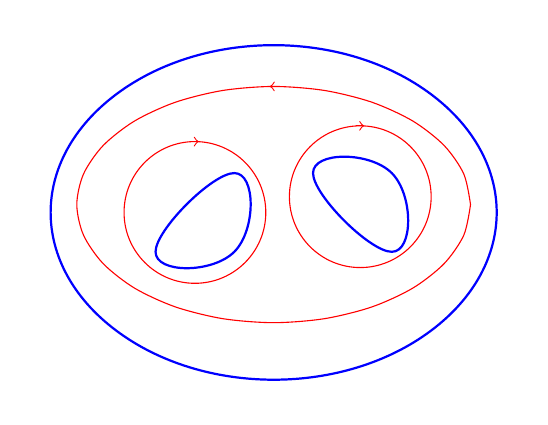
\begin{tikzpicture}
        \draw[blue, thick] plot [smooth cycle, tension=1] coordinates {(0,0) (4,0) (4,3) (0,3)};
        \draw[blue, thick] plot [smooth cycle, tension=1] coordinates {(0.5,1) (1.5,1) (1.5,2)};
        \draw[blue, thick] plot [smooth cycle, tension=1] coordinates {(2.5,2) (3.5,1) (3.5,2)};
        \draw[red] (1, 1.5) circle (0.9);
        \draw[red] (3.1, 1.7) circle (0.9);
        \draw[red,smooth,domain=0:360] plot ({2 + 2.5 * cos(\x)}, {1.6 + 1.5 * sin(\x)});
        \draw[red,->] (0.95, 2.4) -- (1.05, 2.4);
        \draw[red,->] (3.05, 2.6) -- (3.15, 2.6);
        \draw[red,<-] (1.95, 3.1) -- (2.05, 3.1);
%        \draw[darkgreen,domain=5:175] plot ({2 + 2.4 * cos(\x)}, {1.6 + 1.4 * sin(\x)});
%        \draw[darkgreen,domain=185:355] plot ({2 + 2.4 * cos(\x)}, {1.6 + 1.4 * sin(\x)});
%        \draw[darkgreen,domain=5:175] plot ({1 + cos(\x)}, {1.5 + sin(\x)});
%        \draw[darkgreen,domain=185:355] plot ({1 + cos(\x)}, {1.5 + sin(\x)});
%        \draw[darkgreen,domain=5:175] plot ({3.1 + cos(\x)}, {1.7 + sin(\x)});
%        \draw[darkgreen,domain=185:355] plot ({3.1 + cos(\x)}, {1.7 + sin(\x)});
    \end{tikzpicture}\]
    }
    Пусть $\gamma$ --- петля в $\C$, $z_0 \notin \Image(\gamma)$.
    \definition[Индекс пути $\gamma$ относительно $z_0$]{
    Значение интеграла $\frac{1}{2\pi i}\int\limits_{\gamma}\frac{\d z}{z - z_0}$.
    Обозначается $\Ind_{z_0}\gamma$.
    }
    Индекс означает число раз, которые мы обошли вокруг данной точки с учётом ориентации, но пока непонятно даже, почему индекс --- целое число.

    Это определение очевидным образом распространяется на систему путей: $\forall \gamma_j \in \Gamma: z_0 \notin \Image(\gamma) \then$ определён $\Ind_{z_0}\Gamma \bydef \sum\limits_{j = 1}^{n}\frac{1}{2\pi i}\int\limits_{\gamma_j}\frac{\d z}{z - z_0}$
    \properties[Свойства индекса, докажем потом]{
    \item $\Ind_{z_0}\gamma \in \Z$.
    \item Функция $[z_0 \mapsto \Ind_{z_0}\gamma]$ постоянна на каждой компоненте связности $\C \sm \Image(\gamma)$.
    \item На неограниченной компоненте связности $\C \sm \Image(\gamma)$ индекс равен нулю.
    }
    \theorem[Формула вычетов]{
        Пусть $G \subset \C$ --- область, $\Gamma$ --- правильная система путей в $G$, $f: G \sm \{z_1, \dots, z_k\} \map \C$ --- аналитическая функция, и $z_1, \dots, z_k$ --- особенности.
        Если все точки $z_j$ не лежат на носителе системы путей $\Gamma$, то
        \encircle{\int\limits_{\Gamma}f(z)\d z = 2\pi i\left(\sum\limits_{j = 1}^{k}\Res_{z_j}f \cdot \Ind_{z_j}\Gamma\right)}
    \provehere{
    Для каждой точки $z_j$ имеется $r_+$, такой, что $B(z_j, r_+) \sm \{z_j\} \subset G$.
        Тем самым, в окрестности точки $z_j$ функция $f$ разложима в ряд Лорана, и его главная часть сходится везде кроме $z_j$.

    Пусть $g_1, \dots, g_k$ --- главные части рядов Лорана для $f$ в точках $z_1, \dots, z_k$ соответственно.
    Функция $h(z) \coloneqq f(z) - g_1(z) - \dots - g_k(z)$ --- аналитическая функция в области $G$, так как она имеет конечное число особых точек, в которых ограничена.

    Так как $\Gamma$ --- правильная, то $\int\limits_{\Gamma}h(z)\d z = 0$. Тем самым, мы получили
    \[\int\limits_{\Gamma}f(z)\d z = \sum\limits_{j = 1}^{k}\int\limits_{\Gamma}g_j(z)\d z\]
    Посчитаем $\int\limits_{\Gamma}g_j(z)\d z$. Распишем \[g_j(z) = \frac{\Res_{z_j}g}{z - z_j} + \underbrace{\frac{a_1}{(z - z_j)^2} + \dots + \frac{a_{s-1}}{(z - z_j)^s} + \cdots }_{h_j(z)}\]
    У $h_j$ имеется первообразная, так как ряд Лорана можно интегрировать и дифференцировать почленно --- доказательство аналогично оному для степенных рядов.
    Значит, $\int\limits_{\Gamma}g(z)\d z = (\Res_{z_j}f)2\pi i \cdot \Ind_{z_0}\Gamma$ (очевидно, $\Res_{z_j}g_j = \Res_{z_j}f$).
    }
    }
    \newlection{29 марта 2024 г.}
    \subsection{Обобщение интеграла $\frac{\sin x}{x}$}
    Обозначим $\C_+ \bydef \defset{x + iy}{x \in \R, y \in \R_{> 0}}$.

    Пусть $f$ аналитична в $\defset{x + iy}{y > -\eps}$, кроме конечного числа особых точек в $\C_+$, назовём их $z_1. \dots, z_n$.
    В $\defset{x + iy}{-\eps < y < 0}$, получается, у $f$ особенностей нет.

    \proposal{
    Пусть при $\theta \in [0, \pi], R > 0$: $|f(Re^{i\theta})R|$ ограничена в $\C_+$, причём $\forall \theta \in [0, \pi]: \lim\limits_{R \to \infty}f(R e^{i\theta})R = 0$.

        Например, $f(z) = \frac{g(z)}{h(z)}$, где $g, h$ --- многочлены, $\deg g < \deg h$.

        Тогда $\int\limits_{\infty}^{\infty}f(x)\d x = 2\pi i\sum\limits_{j = 1}^{n}\Res_{z_j}f$.
        Здесь $\int\limits_{-\infty}^{\infty} = \lim\limits_{R \to \infty}\int\limits_{-R}^{R}$, то есть особенности несобственного интеграла на плюс-минус бесконечностях могут сокращать друг друга.
    \provehere{
    Проинтегрируем $f$ по синему пути, где полуокружность --- радиуса $R$:
    \[\begin{tikzpicture}
        \draw[->] (-3.5, 0) -- (3.5, 0) node [above right] {$\Re z$};
        \draw[->] (0, -1) -- (0, 3.5) node [above right] {$\Im z$};
        \draw[blue, thick,->] (-2.5, 0) -- (1.5, 0);
        \draw[blue,thick] (1.5, 0) -- (2.5, 0);
        \draw[blue,thick,domain=0:180] plot ({2.5 * cos(\x)}, {2.5 * sin(\x)});
        \draw[blue,thick,->] ({2.5 * 0.6 + 0.05 * 0.8, 2.5 * 0.8 - 0.05 * 0.6}) -- ({2.5 * 0.6 - 0.05 * 0.8, 2.5 * 0.8 + 0.05 * 0.6});
        \draw[blue,thick,->] ({-2.5 * 0.6 + 0.05 * 0.8, 2.5 * 0.8 + 0.05 * 0.6}) -- ({-2.5 * 0.6 - 0.05 * 0.8, 2.5 * 0.8 - 0.05 * 0.6});
        \fill[red] (2, 1) circle (1pt) node[left]{$z_k$};
        \fill[red] (2.2, 0.5) circle (1pt);
        \fill[red] (2.2, 0.7) circle (1pt);
        \fill[red] (-1.2, 0.8) circle (1pt);
        \draw[darkgreen,thick] (-1.2, 0.8) circle (0.3);
        \draw[darkgreen,thick,->] (-0.9, 0.81) -- (-0.9, 0.82);
    \end{tikzpicture}\]
    Пусть $R$ --- настолько большое, что все особые точки в $\C_+$ содержатся во внутренней области, отсекаемой данным путём.
    Оценим интеграл по верхней полуокружности:
    \[\int\limits_{0}^{\pi}f(R e^{it})i R e^{it}\d t \overset{\text{теорема Лебега о мажорируемой сходимости}}{\underset{R \to \infty}\Map} 0\]
    Далее применяем формулу в вычетах.

    Из гомотопности зелёной окружности и синего пути в $\C_+ \sm \{z_j\}$ получаем, что их индексы равны $1$ --- ведь интеграл $\frac{\d z}{z - z_0}$ по окружности мы знаем.
    }
    }
    \subsection{2-я формула замены переменной}
    Пусть $\Phi = f \d x + g \d y$ --- замкнутая дифференциальная форма в $G$, $\gamma: [a, b] \map G$ --- путь, рассмотрим интеграл $\int\limits_{\gamma}\Phi$.
    Изменение параметризации для $\gamma$ --- 1-я формула замены переменной.

    Теперь пусть $g: G_1 \map G_2$ --- голоморфная функция, $f$ --- голоморфная функция в $G_2$, $\gamma: [a, b] \map G_1$ --- непрерывный путь, $\Phi = f(z)\d z$.
    Тогда
    \[\int\limits_{g \circ \gamma}f(z)\d z = \int\limits_{\gamma}(f \circ g)(z) g'(z)\d z\]
    Наводящее соображение: пусть путь $\gamma$ --- кусочно-гладкий, $\rho(t) \coloneqq g(\gamma(t))$.
    Тогда \[\int\limits_{\rho}f(z)\d z = \int\limits_{a}^{b}f(\rho(t))\rho'(t)\d t = \int\limits_{a}^{b}f(g(\gamma(t)))g'(\gamma(t))\gamma'(t)\d t = \int\limits_{\gamma}(f \circ g)(z)\cdot g'(z)\d z\]
    Но нам эта формула пригодится в случае негладкого пути.

    Пусть $\rho = g \circ \gamma$ -- путь в области $G_2$, $\phi$ --- первообразная для формы $f(z)\d z$ вдоль $\rho$.

    Рассмотрим $t_0 \in [a, b]$. $\exists U \ni \rho(t_0)$ --- окрестность, такая, что на ней есть первообразная $\Phi$ для $f(z)\d z$.
    Значит, $\exists \delta > 0: \forall t \in (t_0 - \delta, t_0 + \delta): \phi(t) = \Phi(\rho(t))$.

    Положим $z_0 \coloneqq \gamma(t_0)$. $\exists V \ni z_0: g(V) \subset U$ из непрерывности $g$.
    $\forall w \in U: \Phi'(w) = f(w)$.
    Запишем
    \[\forall z \in V: (\Phi \circ g)'(z) = \Phi'(g(z)) \cdot g'(z)\]
    Тем самым, $\Phi \circ g$ есть первообразная для $(\Phi \circ g) \cdot g'$ в $V$.
    Значит, $\phi \circ g$ --- первообразная для формы $f(g(z)) \cdot g'(z)\d z$ вдоль пути $\gamma$.
    \ok
    Пусть $\gamma$ --- замкнутый путь, не проходящий через $z_0$.
    По определению
    \[\Ind_{z_0}\gamma = \frac{1}{2\pi i}\int\limits_{\gamma}\frac{\d z}{z - z_0}\]
    Применим функцию $[z \mapsto z - z_0]$.
    Согласно 2-й формуле замены переменной,
    \[\Ind_{z_0}\gamma = \frac{1}{2\pi i}\int\limits_{\gamma - z_0}\frac{\d z}{z} = \Ind_{0}(\gamma - z_0)\]
    \corollary{
    Индекс пути $\gamma$ относительно $z_0$ --- локально постоянная функция от $z_0$.
    \provehere{
        Пусть $z_0$ --- точка вне носителя $\gamma$.
        Выберем настолько маленькое $\delta > 0$, что $B(z_0, \delta) \cap \gamma([a, b]) = \o$.

        Рассмотрим $z_1 \in B(z_0, \delta)$, и докажем, что $\Ind_{z_0}\gamma = \Ind_{z_1}\gamma$.
        Определим гомотопию путей $\gamma - z_0$ и $\gamma - z_1$:
        \[\Gamma(t, \tau) \coloneqq (1 - \tau)(\gamma(t) - z_0) + \tau(\gamma(t) - z_1) = \gamma(t) - ((1 - \tau)z_0 + \tau z_1)\]

        Эта гомотопия не проходит через $0$, значит, интегралы по $\gamma - z_0$ и $\gamma - z_1$ равны.
    }
    }
    \corollary{
        Индекс постоянен на каждой компоненте связности $\C \sm \gamma([a, b])$.
    }
    \corollary{
    $\Ind_{z_0}\gamma = 0$ на неограниченной компоненте связности $\C \sm \gamma([a, b])$.
    \provehere{
    Оценим $\int\limits_{\gamma - z_0}\frac{\d w}{w}$ при достаточно большом $|z_0|$. Для такого $z_0$ носитель пути $\gamma - z_0$ лежит в некоторой полуплоскости, не содержащей нуля.
        Полуплосоксть односвязна, это даже звёздная область, в ней путь стягиваем, значит, интеграл равен нулю.
    }
    }
    \subsection{О логарифме}
    Логарифм --- это функция, обратная к экспоненте, а экспонента имеет период $2\pi i$.

    Пусть $w \in \C$.
    \numbers{
    \item Логарифм $w$ --- любое $z \in \C: e^z = w$.
    \item У $w = 0$ логарифма нет;\ если $z$ --- одно из значений логарифма $w$, то все остальные значения имеют вид $\defset{z + 2\pi i k}{k \in \Z}$.
    \item Для $w \ne 0: e = |w|e^{i\theta}$, где $\theta \in \R$.
        Комплексное число $\log|w| + i\theta$ --- одно из значений логарифма.
    }
    Пусть $G$ --- область.
    \definition[Функция $\phi$ в $G$ --- ветвь логарифма в $G$]{
        $\phi$ непрерывна в $G$, и $e^{\phi(z)} = z$ для $z \in G$.
    }
    \fact{
    Всякая ветвь логарифма обязательно голоморфна в $G$, и $\phi'(z) = \frac{1}{z}$.
    \provehere{
%    Согласно вещественной теореме об обратной функции, $\forall z_0 \in \C: \d_z \exp$ невырожден, значит, $\exp$ локально обратима.
%    Значит, локально ветвь логарифма всегда существует.

    Рассмотрим $z_0 \in G, U \coloneqq \defset{z\in\C}{|z - z_0| < \delta} \subset G$.
        Так как производная экспоненты (как вещественной функции $\R^2 \map \R^2$) невырождена, то при достаточно малом $\delta$ у экспоненты имеется обратная $\psi: e^{\psi(z)} = z$ при $z \in U$.

        С другой стороны, $e^{\phi(z)} = z$ при $z \in U$.
    Значит, $\phi - \psi$ --- непрерывная функция, принимающая значения в дискретном множестве $\defset{2\pi i k}{k \in \Z}$.
        Значит, это константа.

    Тем самым, $\phi$ дифференцируема, и $\phi'(z) = \frac{1}{z}$.
    }
    }
    \theorem{
    Во всякой односвязной области $G$: $0 \notin G \then\exists$ непрерывная ветвь логарифма.
    \provehere{
    Напрямую следует из~(\cref{logarithm-in-region}) для тождественного отображения.
    }
    }
    Пусть $F: G \map \C$ --- аналитическая.
    \definition[$\Phi: G \map \C$ --- ветвь логарифма функции $F$]{
        $\forall z \in G: e^{\Phi(z)} = F(z)$.
    }
    \note{
    В определении можно требовать лишь непрерывности $\Phi$, аналитичность получится автоматически.
    }
    \theorem{\label{logarithm-in-region}
    Если $G$ --- односвязная область, $\forall z \in G: F(z) \ne 0$, то в $G$ существует ветвь логарифма для $F$.
    \provehere{
        Функция $\frac{F'(z)}{F(z)}$ --- голоморфна в $G$.
        Форма $\frac{F'(z)}{F(z)}\d z$ замкнута в $G$, значит, имеется первообразная $\phi$ --- голоморфная в $G$ функция, такая, что $\psi'(z) = \frac{F'(z)}{F(z)}$.

    \[\left(\frac{e^{\psi(z)}}{F(z)}\right)' = \frac{e^{\psi(z) \cdot \psi'(z) F(z) - F'(z)e^{\psi(z)}}}{F(z)^2}\]
    По построению $\psi$ числитель равен нулю.
        Тем самым, $e^{\psi(z)} = c \cdot F(z)$.
    $\exists a \in \C: c = e^a$.
        Положим $\phi \coloneqq \psi - a$, это искомая ветвь логарифма.
    }
    }
    \note{
        Не всякая первообразная для $\frac{F'}{F}$ есть ветвь логарифма --- логарифмы отличаются на целые кратные $2\pi i$, а первообразные --- на произвольную константу.
        Однако если $\psi$ --- первообразная $\frac{F'}{F}$, и $\exists z_0\in \C: e^{\psi(z_0)} = F(z_0)$, то $\psi$ --- ветвь логарифма для $F$.
    }
    \note{
    Если $\psi$ --- ветвь логарифма, то все ветви логарифма имеют вид $\defset{\psi + 2\pi i k}{k \in \Z}$.
    }
    Данная функция $\frac{F'}{F}$ называется \emph{логарифмической производной}.

    Пусть $G$ --- область, $f: G \map \C$ --- голоморфна, $\gamma: [a, b] \map G$ --- путь, $\forall z \in \gamma([a, b]): f(z) \ne 0$.

    \definition[Ветвь логарифма вдоль пути $\gamma$]{Функция $\phi: [a, b] \map G$, такая что ${\forall t_0 \in [a, b]}: \exists \delta > 0, \exists U \ni \gamma(t)$, и существует ветвь логарифма $\psi$ функции $f$ в $U$, такая, что
    \[\forall t \in (t_0 - \delta, t_0 + \delta): \phi(t) = \psi(\gamma(t))\]
    }
    \theorem{
    При сделанных предположениях существует ветвь логарифма $f$ вдоль пути $\gamma$. При этом любые две ветви отличаются на $2\pi i k$.
    \provehere{
    Рассмотрим функцию $\frac{f'}{f}$, аналитическую в некоторой окрестности $\gamma([a, b])$.
        Пусть $\phi$ --- первообразная для $\frac{f'}{f}$ вдоль $\gamma$.

        $\forall t_0 \in [a, b]: \exists \delta > 0, \exists U \ni \gamma(t_0)$ вместе с первообразной $\psi$ функции $\frac{f'}{f}$:
    \[\forall t \in (t_0 - \delta, t_0 + \delta): \phi(t) = \psi(\gamma(t))\]
    Существует $c$, вообще говоря, зависящая от $t$, такая, что $e^{\psi(z)} = c f(z)$. При $|t - t_0| < \delta: e^{\phi(t)} = e^{\psi(\gamma(t))} = c f(\gamma(t))$.
    Значит, $\frac{e^\phi(s)}{f(\gamma(s))}$ локально постоянна на $[a, b]$, то есть оказалось, что $c$ всё-таки не зависит от $t$.

        Найдётся $a \in \C: c = e^a$.
        Теперь $\tilde{\phi} \coloneqq \phi - a$ --- тоже первообразная для $\frac{f'}{f}$ вдоль $\gamma$, причём $e^{\psi(\gamma(t)) - a} = f(\gamma(t))$.
        Так как $\psi - a$ --- тоже первообразная в $U$ для $\frac{f'}{f}$, то $\tilde{\psi}$ --- ветвь логарифма.
    }
    }
    В частности, для $f(z) = z - z_0$, и пути $\gamma$, не проходящего через $z_0$, получается ветвь логарифма $z - z_0$ вдоль $\gamma$.
    \comment{Что?}
    \ok
    Пусть $w \in \C$.
    Все значения логарифма спрятаны в формуле $\log w = \log|w| + i \Arg w$, где $\Arg w \bydef \defset{\theta}{e^{i\theta} = \frac{w}{|w|}}$.

    Пусть $G \notin 0$.
    \definition[Непрерывная ветвь аргумента в области $G$]{
    Непрерывная функция $v: G \map \R: \forall z \in G: v(z) \in \Arg(z)$
    }
    \fact{
    В области $G$ существует непрерывная ветвь логарифма $\iff$ в $G$ существует непрерывная ветвь аргумента.
    }
    \definition[Ветвь аргумента вдоль пути $\gamma$]{Функция $\phi: [a, b] \map G$, такая что ${\forall t_0 \in [a, b]}: \exists \delta > 0, \exists U \ni \gamma(t)$, и существует ветвь аргумента $\psi$ функции $f$ в $U$, такая, что
    \[\forall t \in (t_0 - \delta, t_0 + \delta): \phi(t) = \psi(\gamma(t))\]
    }
    В качестве ветви аргумента всегда можно выбрать мнимую часть ветви логарифма.

    Пусть $\gamma: [a, b] \map G$ --- путь, $f: G \map \C$ --- аналитическая, предположим, что $f(z) \ne 0$ на $\gamma([a, b])$.

    Пусть $u$ --- ветвь логарифма для $f$ вдоль $\gamma$.
    \definition[Приращение логарифма вдоль $\gamma$]{
    $u(b) - u(a)$.
    }
    \definition[Приращение аргумента вдоль $\gamma$]{
    $\Im(u(b) - u(a))$.
    }
    Пусть теперь $\gamma$ --- петля.
    Тогда $\Re(u(b) - u(a)) = 0$, и вообще, $u(b) - u(a) = 2\pi i k$ для некоторого $k \in \Z$.
    \newlection{5 апреля 2024 г.}
    \section{Принцип аргумента и теорема Руше}
    Пусть $\gamma: [a, b] \map \C$ --- простой замкнутый путь, $\gamma(a) = \gamma(b)$.
    Положим $D \coloneqq \gamma([a, b])$.
    \intfact[Теорема Жордана]{
    $\C \sm D$ состоит из двух компонент связности.
        Одна из них --- $G$ --- ограничена, и $\forall z \in G: \Ind_{z}\gamma = \pm 1$.
    }
    Если $\Ind_{z}\gamma = 1$, то $\gamma$ называют положительно ориентированной, иначе --- отрицательно ориентированной.
    \definition[Жорданова область]{
    Область, граница которой --- простой замкнутый путь.
    }
%    Чтобы избежать трудностей с доказательством теоремы Жордана
    \theorem[Принцип аргумента]{
        Пусть $G$ --- жорданова область, $\partial G$ --- носитель простого замкнутого пути $\gamma$, ориентированного положительно.

        $f$ --- аналитическая в окрестности $\overline{G}$, кроме, может быть, конечного числа полюсов внутри $G$.
        Более того, $\forall w \in \partial G: f(w) \ne 0$.

        Тогда \[\frac{1}{2\pi} \cdot (\text{приращение аргумента $f$ вдоль $\gamma$}) = (\text{число нулей $f$ в $G$}) - (\text{число полюсов $f$ в $G$})\]
        Нули и полюса надо учитывать с кратностью.
        \provehere{
            Левая часть есть $\frac{1}{2\pi i}\int\limits_{\gamma}\frac{f'(z)}{f(z)}\d z$.
            Это интеграл по простому замкнутому пути; посчитаем его с помощью вычетов $f$ внутри $G$.

            Рассмотрим $z_0 \in G$.
            Пусть вблизи $z_0: f(z) = (z - z_0)^k \cdot g(z)$, где $g$ аналитична вблизи $z_0$, причём $g(z_0) \ne 0$.
        \[f'(z) = k \cdot (z - z_0)^{k - 1}g(z) + (z - z_0)^k g'(z)\quad\then\quad \frac{f'(z)}{f(z)} = \frac{k}{z - z_0} + \frac{g'(z)}{g(z)}\]
        $\frac{g'(z)}{g(z)}$ аналитична в окрестности $z_0$, тем самым, вычет логарифмической производной $\frac{f'(z)}{f(z)}$ в $z_0$ равен $k$.

        Пусть $u_1, \dots, u_s$ --- нули $f$ внутри $G$ кратностей $b_1, \dots, b_s$ соответственно; пусть $v_1, \dots, v_t$ --- полюса $f$ кратностей $l_1, \dots, l_t$ соответственно.
        Суммируя вычеты, получаем $\frac{1}{2\pi i}\int\limits_{\gamma}\frac{f'(z)}{f(z)}\d z = \sum\limits_{j = 1}^{s}k_j - \sum\limits_{j = 1}^{t}l_j$.
        }
    }   \theorem[Теорема Руше]{
            Пусть $G$ --- жорданова область с положительно ориентированной границей --- носителем замкнутого пути $\gamma$.

    Функции $f, g$ аналитичны в окрестности $\overline{G}$.
        Пусть $\forall z \in \partial G: |f(z)| > |g(z)|$.
        В частности, $\forall z \in \partial G: |f(z)| \ne 0, |(f + g)(z)| \ne 0$.

    Тогда $f$ и $f + g$ имеют одинаковое число нулей в $G$.
    \provehere{
        Согласно принципу аргумента, число нулей $(f + g)$ в $G$ равно $\frac{1}{2\pi}\int\limits_{\gamma}\frac{f'(z) + g'(z)}{f(z) + g(z)}\d z$.
     В то же время, $f$ имеет внутри $G$ ровно $\frac{1}{2\pi}\int\limits_{\gamma}\frac{f'(z)}{f(z)}\d z$ нулей.

    Надо доказать, что интегралы равны, вычтем их:
    \[\frac{1}{2\pi i}\int\limits_{\gamma}\left(\frac{f'(z) + g'(z)}{f(z) + g(z)} - \frac{f'(z)}{f(z)}\right)\d z\]
    Теперь преобразуем выражение в скобках:
    \multline{\left(\ddots\right) = \frac{\cancel{f'(z) \cdot f(z)} + g'(z) \cdot f(z) - \cancel{f'(z)\cdot f(z)} - f'(z)\cdot g(z)}{(f(z) + g(z)) \cdot f(z)} =\\= \frac{g'(z)f(z) - f'(z)g(z)}{f(z)^2} \cdot \frac{f(z)}{f(z) + g(z)} = \left(1 + \frac{g(z)}{f(z)}\right)' \cdot \frac{1}{1 + \frac{g(z)}{f(z)}}}
    Обозначим $\Phi(z) \coloneqq 1 + \frac{g(z)}{f(z)}$.
%    \[\circlesign{\coloneq)}\]
    Тем самым, надо доказать, что $\frac{1}{2\pi i}\int\limits_{\gamma}\frac{\Phi'(z)}{\Phi(z)}\d z = 0$.
    При этом, $\forall z \in \partial G: \frac{|f(z)|}{|g(z)|} < 1$.
        Из непрерывности $\exists \delta > 0: \frac{|f(z)|}{|g(z)|} < 1 - \delta$.

    Применим к интегралу формулу замены переменной: $\frac{1}{2\pi i}\int\limits_{\gamma}\frac{\Phi'(z)}{\Phi(z)}\d z = \frac{1}{2\pi i}\int\limits_{\Phi \circ \gamma} \frac{\d w}{w}$.
    При этом носитель пути $\Phi \circ \gamma$ лежит внутри $B(1, 1 - \delta)$, значит, путь гомотопен тождественному, и гомотопия не задевает нуля.
    Действительно, $\frac{1}{2\pi i}\int\limits_{\Phi \circ \gamma} \frac{\d w}{w} = 0$.
    }
    }
    \section{Сходимость аналитических функций}
    Пусть $G \subset \C$ --- открытое множество.
    Пускай $\{h_n\}_{n \in \N}$ --- последовательность функций $h_n: G \map \C$.
    \subsubsection{Равномерная сходимость на компактах}
    Пусть $h: G \map \C$ --- ещё функция.
    Говорят, что $h_n$ сходятся к $h$ ($h_n \underset{n \to \infty}\Map h$), если $\forall$ компакта $K \subset G$: $h_n\big|_K \rightrightarrows h\big|_K$.

    В дальнейшем, говоря о сходимости аналитических функций, будем подразумевать именно равномерную сходимость на компактах.
    \theorem[Вейерштрасс, 1-я]{
        Пусть все $h_n: G \map \C$ --- аналитичны, и $h_n \underset{n \to \infty}\Map h$.
        Тогда $h$ аналитична в $G$.
        \provehere{
            Достаточно доказать, что $\forall$ прямоугольника $\overline{P} \subset G: \int\limits_{\partial P}h(z)\d z = 0$.
            Это ясно из равномерной сходимости на компактах:
            \[\abs{\,\int\limits_{\partial P}(h(z) - h_n(z))\d z} \le \sup\limits_{z \in \partial P}|h_n(z) - h(z)| \cdot l(\partial P)\]
            Далее достаточно применить теорему Мореры~(\cref{morera}).
        }
    }
    \theorem[Вейерштрасс, 2-я]{
        Пусть все $f_n: G \map \C$ --- аналитичны, и $f_n \underset{n \to \infty}\Map f$, где аналитичная $f: G \map \C$.
        Тогда $f_n' \underset{n \to \infty}\Map f'$.
        \provehere{
            Пусть $K = DB(w_0, r)$ --- круг, $\overline{K} \subset G$.
            Понятно, $\exists R > r: \overline{B(w_0, R)} \subset G$.
            Рассмотрим $z \in K$.
        \[f_n'(z) = \frac{1}{2\pi i}\int\limits_{|\zeta - w_0| = R}\frac{f_n(\zeta)}{(\zeta - z)^2}\d\zeta \underset{n \to \infty}\Map \frac{1}{2\pi i}\int\limits_{|\zeta - w_0| = R}\frac{f(\zeta)}{(\zeta - z)^2}\d\zeta = f'(z)\]
        К пределу под интегралом можно перейти, так как сходимость равномерна в $\overline{K}$, знаменатель отделён от нуля числом $R - r$.
        Более того, видно, что сходимость равномерна в $\overline{K}$.

        Пусть $S \subset G$ --- компакт. $\forall s \in S: \exists K_s$ --- круг с центром в $s$, такой, что $\overline{K}_s \subset G$.
        Внутренности этих кругов покрывают $S$, выберем конечное подпокрытие.

            На каждом из кругов конечного подпокрытия имеется равномерная сходимость.
            Стало быть, имеется равномерная сходимость на $S$.
        }
    }
    \lemma{
        Пусть $f_n, f$ --- аналитические функции в области $G$, $f_n \underset{n \to \infty}\Map f$, $f$ не равана тождественному нулю.

    Пусть $D$ --- круг, $D \subset G$, предположим, что $f$ имеет нуль в $D$.
        Тогда для всех достаточно больших $n$: $f_n$ имеет нуль в круге $D$.
    \provehere{
    Пусть $f(z_0) = 0$.
        Уменьшая $D$, можем считать, что $D = B(z_0, r)$ --- круг, такой, что $\overline{D} \subset G$.

        По теореме единственности $f$ не постоянна в $D$.

        Разложим $f$ в ряд Тейлора в $D$:
    \[f(z) = a_0 + a_1 (z - z_0) + a_2 (z - z_0)^2 + \cdots\]
    Ряд сходится в некоторой окрестности $\overline{D}$. $a_0 = 0$, но не все коэффициенты равны нулю. Распишем
    \[f(z) = (z - z_0)^k \cdot g(z), \quad g(z_0) \ne 0\text{, где $g$ аналитична в окрестности $\overline{D}$}\]

    Пусть $\rho \le r$ выбрано так, что $\forall z: |z - z_0| \le \rho \then |g(z)| > \delta > 0$.
    Оценим $f$ при $|z - z_0| = \rho: |f(z)| = |z - z_0|^k \cdot |g(z)| \ge \rho^k \delta$.

    Разложим $f_n(z) = f(z) + (f_n(z) - f(z))$.
        При достаточно больших $n: |f_n(z) - f(z)| < \rho^k\delta$, по теореме Руше $f_n$ имеет нуль внутри $D$.
    }
    }

    \definition[Однолистная функция $f: G \map \C$]{Инъективная аналитическая функция $f$.}
    \theorem{
        Пусть $f_n$ --- последовательность однолистных функций в области $G$, $f_n \underset{n \to \infty}\Map f$.
    Тогда либо $f \equiv \const$, либо $f$ --- тоже однолистна.
    \provehere{
        Предположим, что $\exists z_0, z_1 \in G: z_0 \ne z_1$ и $w \coloneqq f(z_0) = f(z_1)$.
    Построим $g(z) \coloneqq f(z) - w, g_n(z) \coloneqq f(z) - w$.
        Сходимость сохранилась.

    Пусть $U_0, U_1$ --- круги с центрами в $z_0$ и $z_1$ соответственно, $U_0 \cap U_1 = \o, U_0, U_1 \subset G$.
    Функция $g$ имеет нуль в каждом из $U_1, U_2$.
        Предположим, что $g \not\equiv 0$, значит, при достаточно большом $n: g_n$ имеет нуль как в $U_1$, так и в $U_2$.
        Но $g_n$ однолистна, значит, всё же $g \equiv 0$.
    }
    }
    \theorem[Риман]{
        Пусть $G \subset \C$ --- область.
        Следующие условия эквивалентны:
    \numbers{
    \item $G$ односвязна, $G \ne \C$.
    \item $\exists$ однолистная $\phi: G \twoheadrightarrow \D = \defset{z \in \C}{|z| < 1}$.
    }
    \provehere{
    Потом.
    }
    }
    \subsection{Нормальные семейства}
    Пусть дано множество $A$ аналитичных функций в области $G$.
    \definition[Нормальное множество $A$]{
    Такое $A$, что $\forall$ компакта $K \subset G: \exists C \in \R: \forall z \in K, \forall f \in A: |f(z)| \le C$.
    }
    \theorem{
    Следующие условия эквивалентны:
    \numbers{
    \item Множество $A$ нормально.
    \item $\forall \{f_n\}_{n \in \N}, f_n \in A$: найдётся сходящаяся подпоследовательность $n_1 < n_2 < \dots: {\exists f: f_{n_j} \underset{j \to \infty}\Map f}$.
    \provebullets{
    \item[$(2) \then (1)$] Предположим противное: $\exists K \subset G: \forall m \in \N: \exists f_m \in A: \sup\limits_{z \in K}|f_m(z)| > m$.

    Согласно посылке, существует сходящаяся подпоследовательность $\{m_k\}_{k \in \N}$, такая, что $\exists f: f_{m_k} \underset{k \to \infty}\rightrightarrows f$ равномерно на $K$.
        $f$ ограничена на $K$, значит, начиная с некоторого места, $f_{m_k}$ тоже ограничены.
        Противоречие.
    \item[$(1) \then (2)$]
    \indentlemma{
    Рассмотрим счётный набор последовательностей \[\all{x_1^{(1)}, x_2^{(1)}, x_3^{(1)}, \dots \\ x_1^{(2)}, x_2^{(2)}, x_3^{(2)}, \dots \\ x_1^{(3)}, x_2^{(3)}, x_3^{(3)}, \dots \\ \ddots }\]
    Пусть каждая последовательность ограничена: $\forall n \in \N: \exists M^{(n)}: \forall j: |x_j^{(n)}| < M^{(n)}$.
    Тогда $\exists k_1 < k_2 < \dots$ --- подпоследовательность индексов, такая, что $\forall n \in \N: \exists x^{(n)}: x^{(n)}_{k_j} \underset{j \to \infty}\Map x^{(n)}$.
    }{
    Пусть $\{k^{(1)}_j\}_{j \in \N}$ --- такая подпоследовательность индексов, что $\exists x^{(1)}: x_{k^{(1)}_j} \underset{j \to \infty}\Map x^{(1)}$.
    Выберем из этой последовательности индексов подпоследовательность индексов $\{k^{(2)}_j\}_{j \in \N}$, что $\exists x^{(2)}: x^{k^{(2)}_j} \underset{j \to \infty}\Map x^{(2)}$.
    И так далее.

    Тем самым, мы получим счётное количество последовательностей индексов, таких, что $k^{(n + 1)}$ --- подпоследовательность $k^{(n)}$, и $\forall n \in \N: \exists x^{(n)}: x_{k^{(n)}_j} \underset{j \to \infty}\Map x^{(n)}$.

    А теперь возьмём диагональ: $k_j \coloneqq k^{(j)}_j$.
    }
    }
    }
    }
    \newlection{12 апреля 2024 г.}
    todo
    \newlection{19 апреля 2024 г.}
    \theorem[Риман]{
        Пусть $G \subset \C$ --- область.
        Следующие условия эквивалентны:
        \numbers{
            \item $G$ односвязна, $G \ne \C$.
            \item $\exists$ однолистная сюръекция $\phi: G \twoheadrightarrow \D = \defset{z \in \C}{|z| < 1}$.
        }
        \provehere{
            На прошлой лекции свели к случаю $G \subset \D, G \ni 0$.

            Введём $\mathcal{A} \coloneqq \defset{f: G \map \D}{f(0) = 0\text{ и $f$ однолистна}}$.
            Доказали, что существует $f \in \mathcal{A}$, такая, что $|f'(0)|$ максимально.

            Далее пойдём от противного: пусть $\exists a \in \D: a \notin \Image(f)$.
        Введём $\phi \coloneqq v \circ f$, где $v(w) \coloneqq \frac{w - a}{1 - \overline{a}w}$ --- некоторое преобразование Мёбиуса.
            $\phi(z) \coloneqq \frac{f(z) - a}{1 - \overline{a}f(z)}$.

        К сожалению, пока $\phi \notin \mathcal{A}: \phi(0) \ne 0$, и вообще $\phi(z) \ne 0$ везде.
        Но раз так, то у $\phi$ имеется ветвь логарифма $\Phi$.
            Так как $\Re\log(u) = \log|u|$, то $\forall z \in G: \Re\Phi(z) < 0$.
            При помощи другого дробно-линейного преобразования переведём левую полуплоскость обратно в $\D: g(z) \coloneqq \frac{\Phi(z) - \Phi(0)}{\Phi(z) + \overline{\Phi(0)}}$.
        Утверждается, что $g \in \mathcal{A}$: $g(0) = 0$, и преобразование $w \mapsto \frac{w - a}{w + \overline{a}}$ однолистно стреляет в круг $\D$.

        Осталось получить противоречие, получив в результате вычислений, что $|g'(0)| > |f'(0)|$.
        \multline{
        g'(z) = \left(1 - \frac{2\Re\Phi(0)}{\Phi(z) + \overline{\Phi(0)}}\right)' = \frac{2\Re(\Phi(0))}{(\Phi(z) + \overline{\Phi(0)})^2}\Phi'(z) = \frac{2\Re(\Phi(0))}{(\Phi(z) + \overline{\Phi(0)})^2}\frac{\phi'(z)}{\phi(z)} = \\
        = \frac{2\Re(\Phi(0))}{(\Phi(z) + \overline{\Phi(0)})^2}\frac{1}{\phi(z)} \cdot \frac{(1 - \overline{a}f(z)) \cdot f'(z) + \overline{a} \cdot f'(z)(f(z) - a)}{(1 - \overline{a}f(z))^2}
        }
Подставляя $0$, получаем
        \[g'(0) = \frac{2\Re\Phi(0)}{(2\Re\Phi(0))^2}\frac{1}{-a} \cdot \frac{f'(0)(1 - |a|^2)}{1}\]
        Тем самым, $|g'(0)| = \frac{1}{2 \log\left(\frac{1}{|a|}\right)}\frac{1 - |a|^2}{|a|} \cdot |f'(0)|$.
        Осталось убедиться, что для $t \coloneqq |a| \in (0, 1)$ выполнено неравенство $\frac{1 - t^2}{2t \log\left(\frac{1}{t}\right)} > 1$.
        Это эквивалентно неравенству $\frac{1 - t^2}{t} - 2\log\left(\frac{1}{t}\right) > 0$.
            При $t = 1$ левая часть равняется нулю, и производная левой части $\left(\frac{1}{t} - t + 2\log\left(t\right)\right) = -\frac{1}{t^2} - 1 - \frac{2}{t} = -\left(\frac{1}{t} - 1\right)^2 < 0$.
        }
    }
    Пусть $f_1, f_2: G \twoheadrightarrow \D$ --- возможно различные однолистные отображения.
    Тогда $f_2^{-1} \circ f_1$ --- однолистное отображение круга $\D$ на себя.
    Например, это может быть каким-то преобразованием Мёбиуса, но оказывается, что ими всё и исчерпывается.
    \definition[Автоморфизм области $G$]{
    Однолистное отображение $G \twoheadrightarrow G$.
    }
    Вообще практически все односвязные области эквивалентны (при помощи однолистной сюръекции) кругу, как говорит только что доказанная теорема Римана, но есть ещё две области --- $\C$ и $\hat{\C}$, имеющие другую природу.

    Сначала займёмся автоморфизмами $\C$.
    \theorem{
    Автоморфизмы $\C$ --- линейные функции $z \mapsto az + b$ при $a \ne 0$.
    \provehere{
    Пускай $f: \C \twoheadrightarrow \C$ --- ещё какой-то автоморфизм $\C$.
        Тем самым, $f$ --- целая, то есть $f = a_0 + a_1 z + \dots$

    Если $a_j \ne 0$ для бесконечного множества индексов $j$, то $\infty$ --- существенно особая точка (в ряду Лорана $f\left(\frac{1}{z}\right)$ бесконечно много ненулевых членов).
    Так как $\forall z \in \C: f'(z) \ne 0$, то $f$ --- открытое отображение.
        Отсюда $f(\D)$ открыто.
        С другой стороны, по теореме Сохоцкого $f(\defset{z \in \C}{|z| > 1})$ всюду плотно в $\C$. Значит, $\exists w \in f(\D) \cap f(\defset{z \in \C}{|z| > 1})$, и это противоречие с однолистностью $f$.

        Тем самым, $f$ --- многочлен, и если $\deg f \ge 2$, то $f'$ имеет корень, опять-таки противоречие с однолистностью.
        Получается, $f$ --- линейная функция, или константа, но константа не подходит.
    }
    }
    \note{
    $\hat{\C}$ односвязна, так как топологически это --- сфера, что видно из стереографической проекции.
    }
    \theorem{
    Автоморфизмы $\hat{\C}$ --- дробно-линейные отображения $z \mapsto \frac{az + b}{cz + d}$ при $ad - bc \ne 0$.
    \provehere{
        \indentlemma[О действии групп]{
            Пусть группа $\Gamma$ действует на множестве $X$;\\ $H \le X$ --- подгруппа.
        Если $\exists x \in X: H \supset \Gamma_x$ ($\Gamma_x \bydef \defset{\gamma \in \Gamma}{\gamma x = x}$ --- стабилизатор $x$), и $H$ действует на $X$ транзитивно ($\forall x, y \in X: \exists \gamma \in H: \gamma x = y$), то $H = \Gamma$.
        }{
            Рассмотрим какой-то $\gamma \in \Gamma$.
            Пусть $\gamma(x) = y$. Из транзитивности $\exists \delta \in H: \delta y = x$. Тем самым, $\delta\gamma x = x$, то есть $\delta\gamma \in H \then \gamma \in H$.
        }
    }
        Введём в качестве $\Gamma$ группу всех однолистных отображений $\hat{C} \twoheadrightarrow\hat{C}$, и в качестве $H \le \Gamma$ --- подгруппу дробно-линейных отображений.

        Легко видеть, что $H$ действует на $\C$ транзитивно: скажем, любая точка лежит в одной орбите с $\infty$: $\forall z_0 \in \C: \frac{1}{z - z_0}\Big|_{z = z_0} = \infty$.
        С другой стороны, стабилизатор $\infty$ --- автоморфизмы $\C$, и так как они лежат в $H$, то $H = \Gamma$.
    }
    \lemma[Шварц]{
    Пусть $f: \D \map \D$ --- аналитическая функция, такая, что $f(0) = 0$.
        Тогда $\forall z \in \D: |f(z)| \le |z|$. При этом если $\exists z \in \D \sm \{0\}: |f(z)| = |z|$, то $\exists c \in \C \:(|c| = 1): f(z) = cz$.
    \provebullets{
    \item Пусть дополнительно $f$ задана в круге радиуса $R > 1$ с центром в $0$.
    Рассмотрим $g(z) \coloneqq \frac{f(z)}{z}$ --- она аналитична в круге $\defset{z \in \C}{|z| < R}$, так как в нуле --- устранимая особенность.

    При $|z| = 1: |g(z)| = \frac{|f(z)|}{|z|} \le \frac{1}{1} = 1$.
        Согласно принципу максимума модуля~(\cref{maximum-on-boundary}), $|g| \le 1$ везде.
    \item Теперь такого предположения о $f$ не имеется.
        Выберем $R > 1$. Определим $f_R(z) \coloneqq f\left(\frac{z}{R}\right)$.
        Согласно предыдущему пункту $\forall z \in \D: |f_R(z)| \le |z|$. Устремляя $R \to 1$, получаем искомое неравенство.
    \item Осталось разобраться со случаем равенства внутри круга.
        Пусть $\exists z_0 \in \D \sm \{0\}: |f(z_0)| = |z_0|$.
        Тем самым, $g(z) \coloneqq \frac{f(z)}{z}$ достигает своё наибольшее значение внутри круга, то есть $g \equiv c = \const$.
        Подставляя $z_0$, получаем $|c| = 1$.
    }
    }
    Пусть $\Gamma$ --- группа всех автоморфизмов круга $\D$.
    Вычислим стабилизатор $0 \in \D$.
    Пусть $\phi \in \Gamma_0$ --- аналитическая биекция, такая, что $\phi(0) = 0$.
    То же верно и для $\phi^{-1}$.

    По лемме Шварца $|\phi(z)| \le |z|$, но применяя её же к $\phi^{-1}$, получаем $z = \phi^{-1}(\phi(z)) \then |z| = |\phi^{-1}(\phi(z))| \le |\phi(z)|$.
    Тем самым, $|\phi(z)| = |z|$ во всех точках, и по лемме Шварца $\phi$ --- гомотетия с коэффициентом $c\: (|c| = 1)$.

    Группа преобразований Мёбиуса $\defset{w \mapsto c \cdot \frac{w - a}{1 - \overline{a}w}}{a \in \D, |c| = 1}$ содержит при $a = 0$ гомотетии с данными коэффициентами, и действует транзитивно на $\D$: любая $a \in \D$ переводится соответствующим преобразованием в нуль.
%   Проверим, что это группа: \[\left[\arr{cc}{c_1 & -a_1 c_1 \\ -\overline{a}_1 & 1}\right] \cdot \left[\arr{cc}{c_2 & -a_2 c_2 \\ -\overline{a}_2 & 1}\right] = \left[\arr{cc}{c_1 c_2 + a_1 \overline{a}_2 c_1 & -a_2 c_1 c_2  - a_1 c_1 \\ -\overline{a}_1 c_2 - \overline{a}_2 & \overline{a}_1 a_2 c_2 + 1}\right] = \left[\arr{cc}{c_1\frac{c_2 \overline{a}_1 a_2 + |a_1|^2 |a_2|^2}{\overline{a}_1 a_2 c_2 + 1}&\\3&1}\right]\]
    \exercise{Проверить, что группа Мёбиуса --- действительно группа, то есть замкнута относительно умножения и взятия обратного.}
    \fact[Конформность однолистного отображения]{
        Пусть $G$ --- область, $z_0 \in G$, $\Phi: G \map G$ --- однолистные отображения.
        Пусть $\gamma_1, \gamma_2: (-\eps, \eps) \map G$ --- два регулярно параметризованных пути ($\gamma_1' \ne 0, \gamma_2' \ne 0$), причём $\gamma_1(t_1) = \gamma_2(t_2) = z_0$.
        Проводя касательные к носителям $\gamma_1, \gamma_2$ в $z_0$, получаем угол, его косинус можно посчитать по формуле $\frac{\angles{\gamma_1'(t_1), \gamma_2'(t_2)}}{|\gamma_1'(t_1)|\cdot|\gamma_2'(t_2)|}$.

        Подействуем при помощи $\Phi$ на данную картинку. $\tilde{\gamma}_j \coloneqq \Phi \circ \gamma_j$ при $j \coloneqq 1, 2$.
        Несложно посчитать, что $\tilde{\gamma}_j'(t_j) = \Phi'(z_0) \cdot \gamma_j'(t_j)$, что действительно сохраняет косинус угла.
    }
    Такие отображения, сохраняющие углы, называют \emph{конформными}.
    В силу исторических причин, говоря про однолистные отображения, часто добавляют слово <<конформные>>, а сама наука зовётся теорией конформных отображений, хотя, как мы только что видели, однолистность сильнее.
    \section{Целые функции}
    \definition[Целая функция]{Аналитическая $\C \map \C$.}
    \subsection{Построение целых функций с заданными нулями}
    Пусть $f \not\equiv 0$ --- целая, $N \coloneqq \defset{a \in \C}{f(a) = 0}$.
    По теореме единственности $N$ не имеет предельных точек.
    В частности, все нули изолированы, откуда множество нулей не более, чем счётно.

    Нули удобно считать с учётом кратности, получая при этом мультимножество $N$.

    Пронумеруем $N = \{a_0, a_1, a_2, \dots\}$, удобно считать, что $|a_0| \le |a_1| \le \dots$.
    \theorem[Вейерштрасс]{
        Существует целая функция $f$, мультимножество нулей которой совпадает с данным мультимножеством $N = \{a_0, a_1, \dots\}$.
        Считаем $|a_0| \le |a_1| \le \dots$.
        Дополнительно предполагается, что $|a_j| \underset{j \to \infty}\Map \infty$.
        \comment{Кажется, это необходимое и достаточное условие того, что у $N$ нет предельных точек}
        \provehere{
            Если бы нулей было конечное количество, то многочлен $(z - a_0) \proddots (z - a_N)$ подошёл бы, но нулей, увы, бесконечно.
            Предположим, что $0 \notin N$ (это не ограничивает общность: выкинем $0$ из $N$, построим $f$, потом домножим на нужную степень $z^k$), и заметим, что произведение $\left(1 - \frac{z}{a_0}\right) \proddots \left(1 - \frac{z}{a_N}\right)$ тоже решает задачу в случае конечного $N$.

            В бесконечном же случае стоит озаботиться вопросом сходимости.
            Во втором семестре мы проверяли, что сходимость $\prod\limits_{j = 0}^{\infty}a_j$ \textbf{не к нулю} эквивалентна сходимости ряда $\sum\limits_{j = 0}^{\infty}\log (a_j)$, где $\log: \left(\C \sm (-\infty, 0]\right) \map \C$ --- главная ветвь логарифма.

            Рассмотрим бесконечное произведение $\prod\limits_{j = 0}^{\infty}u_j(z)$, где $u_j$ --- аналитические функции.
            Будем говорить, что данное \emph{произведение сходится}, если $\forall$ компакта $K \subset G: \exists M \in \N: \forall j \ge M, z \in K: u_j(z) \ne 0$, и произведение $\prod\limits_{j > N}u_j(z)$ сходится на $K$ равномерно.
        
            Определим \emph{множители Вейерштрасса}: \[u_j(z) \coloneqq \left(1 - \frac{z}{a_j}\right) \cdot \exp\left(-\left(\frac{z}{a_j} + \frac{1}{2}\left(\frac{z}{a_j}\right)^2 + \dots + \frac{1}{j - 1}\left(\frac{z}{a_{j-1}}\right)^{j-1}\right)\right)\]
            Показатель экспоненты подогнан так, чтобы при взятии логарифма много чего сократилось (а $\log(1 - w) = w + \frac{w^2}{2} + \frac{w^3}{3} + \dots$ при $|w| < 1$, например, потому что этот ряд совпадает с рядом для вещественного логарифма на $\R_{> 0}$, и имеется теорема единственности)

            Осталось показать, что произведение $\prod\limits_{j = 0}^{\infty}u_j(z)$ сходится равномерно на компактах, и её нули --- в точности $a_j$ с учётом кратности.

            Определим компакт $K \coloneqq \defset{z \in \C}{|z| \le \frac{|a_N|}{2}}$, и покажем, что $\prod\limits_{j > N}u_j(z)$ сходится равномерно на $K$.
            \[u_j(z) = \exp\left(\log\left(1 - \frac{z}{a_j}\right) - \frac{z}{a_j} - \dots - \frac{1}{j - 1}\left(\frac{z}{a_j}\right)^{j - 1}\right) = \exp\left(\sum\limits_{s \ge j}\frac{1}{s}\left(\frac{z}{a_j}\right)^s\right)\]
            При этом $\log\left(1 - \frac{z}{a_j}\right)$ определён, так как $|z| < |a_j|$. Оценим
            \[\abs{\sum\limits_{s \ge j}\frac{1}{s}\left(\frac{z}{a_j}\right)^s} \le \abs{\sum\limits_{s \ge j}\left(\frac{z}{a_j}\right)^s}\le \abs{\sum\limits_{s \ge j}\left|\frac{a_N}{2a_j}\right|^s} \le \left(\frac{1}{2}\right)^j\]

            Убедимся, что ряд из логарифмов равномерно сходится:
            \[\abs{\sum\limits_{j > N}\sum\limits_{s \ge j}\frac{1}{s}\left(\frac{z}{a_j}\right)^s} \le \sum\limits_{j \ge N}\left(\frac{1}{2}\right)^j \le 1\]
            Получатся, данное произведение $\prod\limits_{j \ge 0}u_j(z)$ подходит.
        }
    }
    \newlection{26 апреля 2024 г.}
    \subsection{Упрощённый вид множителей Вейерштрасса}
    Если известно, насколько быстро происходит стремление $|a_j|\underset{j \to \infty}\Map \infty$, то можно утверждать наличие сходимости и при множителях Вейерштрасса более простого вида.
    \numbers{
    \item Если $\sum\limits_{n \ge 0}\frac{1}{|a_n|} < \infty$, то никаких премудростей не надо: $\prod\limits_{j = 1}^{\infty}\left(1 - \frac{z}{a_j}\right)$ сходится.
    \provehere{
        Зафиксируем $N \in \N$, и рассмотрим компакт $K \coloneqq \bigdefset{z \in \C}{|z| \le \frac{1}{2}a_N}$.
        Надо доказать, что $\sum\limits_{j \ge N}\log\left(1 - \frac{z}{a_j}\right)$ сходится.

        Под логарифмом стоят выражения вида $1 - t$, где $|t| \le \frac{1}{2}$.
        Разложим в ряд и оценим: $\log(1 - t) = t + \frac{t^2}{2} + \frac{t^3}{3} + \dots = t\left(1 + \frac{t}{2} + \frac{t^2}{3} + \dots\right) \le t \cdot C$, где $C \coloneqq \sum\limits_{n \ge 1}\frac{\left(\nicefrac12\right)^{n-1}}{n}$.
        Этой оценки достаточно: $\sum\limits_{j \ge N}\abs{\log\left(1 - \frac{z}{a_j}\right)} \le \sum\limits_{j \ge N}C\abs{\frac{z}{a_j}}$, что сходится равномерно по $z \in K$.
    }
    \item Если $\sum\limits_{n \ge 0}\frac{1}{|a_n|^2} < \infty$, то хватит первого члена при разложении логарифма в ряд: $\prod\limits_{j = 1}^{\infty}\left(1 - \frac{z}{a_j}\right)e^{\frac{z}{a_j}}$ сходится.
        \provehere{
            Зафиксируем $N \in \N$, и рассмотрим компакт $K \coloneqq \bigdefset{z \in \C}{|z| \le \frac{1}{2}a_N}$.
            Надо доказать, что $\sum\limits_{j \ge N}\log\left(1 - \frac{z}{a_j}\right)\cdot{\frac{z}{a_j}}$ сходится.

            Разложим в ряд и оценим: $\log(1 - t)t = t^2 + \frac{t^3}{2} + \frac{t^4}{3} + \dots = t^2\left(1 + \frac{t}{2} + \frac{t^2}{3} + \dots\right) \le t^2 \cdot C$, где $C \coloneqq \sum\limits_{n \ge 1}\frac{\left(\nicefrac12\right)^{n-1}}{n}$.
            Этой оценки достаточно: $\sum\limits_{j \ge N}\abs{\log\left(1 - \frac{z}{a_j}\right)\frac{z}{a_j}} \le \sum\limits_{j \ge N}C\abs{\frac{z}{a_j}}^2$, что сходится равномерно по $z \in K$.
        }
    }
    \note{
    Понятно, что целая функция с данным мультимножеством нулей не единственна --- можно взять любую другую целую функцию без нулей (скажем, экспоненту), и домножить на неё.
    }
    \corollary{
    Пусть $f: \C \map \C$ --- целая функция с бесконечным числом нулей, и $g$ --- произведение Вейерштрасса по нулям функции $f$ (неважно, общего вида, или с упрощёнными множителями).

    Тогда $\exists$ целая $h: \C \map \C$: $f = g e^h$.
    \provehere{
        $\frac{f}{g}$ --- целая функция (там, где у $g$ нули, у $f$ --- нули той же кратности, поэтому все особенности устранимы).
        По той же причине $\forall z \in \C: \frac{f}{g}(z) \ne 0$.
        Тем самым, у неё есть ветвь логарифма, выберем какую-то ветвь $h$, она как раз подходит.
    }
    }
    Пусть $G$ --- область, $f$ аналитична в $G$ кроме некоторого множества полюсов.
    Такая функция называется \emph{мероморфной в $G$}.
    Так как полюса по определению изолированы, то их не более, чем счётное количество.

    Мероморфную в $\C$ функцию называют мероморфной.
    \corollary{
    $f$ мероморфна $\iff \exists$ целые $g_1, g_2: f = \frac{g_1}{g_2}$.
    \provehere{
    Рассмотрим функцию $\frac{1}{f}$.
        Она не равна тождественно нулю.

    Пусть $g$ --- произведение Вейерштрасса по нулям функции $\frac{1}{f}$, $g \cdot f$ --- целая функция.
    }
    }
    \subsection{Разложение синуса в произведение}
    Разложим синус в произведение, построив произведение Вейерштрасса по его нулям.
    А где нули синуса?
    $\sin z = \frac{e^{iz} - e^{-iz}}{2}$.
    \[\sin z = 0 \iff e^{iz} = e^{-iz} \iff e^{2iz} = 1 \iff z \in \defset{j \cdot \pi}{j \in \Z}\]
    Как видим, сумма обратных квадратов сходится, поэтому можно записать произведение Вейерштрасса в виде
    \[z\cdot\prod\limits_{j \in \Z \sm \{0\}}\left(1 - \frac{z}{j \pi}\right)e^{\frac{z}{j\pi}}\]
    где произведение берётся в порядке возрастания модулей $j$.
    Иными словами, \[z \cdot \lim\limits_{N \to \infty}\prod\limits_{\substack{j \le N \\ j \ne 0}}\left(1 - \frac{z}{j \pi}\right)e^{\frac{z}{j\pi}} = z \cdot \lim\limits_{N \to \infty}\prod\limits_{j = 1}^{N}\left(1 - \frac{z^2}{j^2 \pi^2}\right) = z \prod\limits_{j = 1}^{\infty}\left(1 - \frac{z^2}{j^2 \pi^2}\right)\]
    Как мы выяснили, $\exists$ целая $h: \C \map \C: \sin(z) = e^{h(z)} z \prod\limits_{j = 1}^{\infty}\left(1 - \frac{z^2}{j^2 \pi^2}\right)$
    \fact{
    $h \equiv 0$ подойдёт (понятно, что если это правда, то $2\pi i k$ для $k \in \Z$ тоже подойдёт).
    \provehere{
        \indent{\note[О логарифмической производной]{
            Пусть $\phi$ --- аналитическая функция, как известно, её логарифмическая производная $\frac{\phi'}{\phi}$.
            Как видно из записи, она не зависит от того, какая ветвь логарифма где взята.

            Если $\phi = \phi_1 \proddots \phi_k$, то несложно посчитать, что $\frac{\phi'}{\phi} = \frac{\phi_1'}{\phi_1} + \dots + \frac{\phi_n'}{\phi_n}$.
            Утверждается, что формула сохраняется и для бесконечного произведения.

            Пусть произведение $\prod\limits_{j = 1}^{\infty}\phi_j(z)$ сходится равномерно на любом компакте, не содержащем нулей функций $\phi_j$.
        Пусть $K$ --- такой компакт, то есть $(\phi_1 \proddots \phi_n)(z) \rightrightarrows \phi(z)$ равномерно.
            Тогда $(\phi_1 \proddots \phi_N)'(z) \rightrightarrows \phi'(z)$ на этом же компакте, и как следствие, $\frac{\phi_1'(z)}{\phi_1(z)} + \dots + \frac{\phi_N'(z)}{\phi_N(z)} = \frac{(\phi_1\proddots \phi_N)'(z)}{(\phi_1\proddots \phi_N)(z)} \rightrightarrows \frac{\phi'(z)}{\phi(z)}$
        }
        }
        \bullets{
            \item Возьмём логарифмическую производную обеих частей равенства $\sin(z) = e^{h(z)} \cdot z \cdot \prod\limits_{\substack{|j| \le N, j \ne 0}}\left(1 - \frac{z}{j\pi}\right)$:
            \[\frac{\cos z}{\sin z} = h'(z) + \frac{1}{z} - \lim\limits_{N \to \infty}\sum\limits_{\substack{|j| \le N, j \ne 0}}\frac{1}{j\pi}\frac{1}{1 - \frac{z}{j\pi}} = h'(z) + \frac{1}{z} + \lim\limits_{N \to \infty}\sum\limits_{\substack{|j| \le N, j \ne 0}}\frac{1}{z - j\pi}\]
            Отлично, у нас имеется равномерная сходимость на компактах, продифференцируем ещё раз:
            \[1-\ctg(z)^2 = h''(z) - \frac{1}{z^2} - \lim\limits_{N \to \infty}\sum\limits_{\substack{|j| \le N, j \ne 0}}\frac{1}{\left(z - j\pi\right)^2}\]
            \item Проведём окружность $\Gamma_k$ с центром в нуле, и радиусом $\pi\left(k + \frac{1}{2}\right)$, и докажем, что $h''$ ограничена на $\Gamma_k$ некоторой константой $C$, не зависящей от $k$.

            Понятно $\frac{1}{z^2} \le \frac{4}{\pi^2}$, оценим при $z \in \Gamma_k: \frac{1}{|z - j\pi|^2} \le \frac{1}{(k + \frac{1}{2} - |j|)^2\pi^2}$.
            \comment{Кажется, это не совсем правда, но может и вообще правда.}
            Осталось оценить котангенс:
            \[\ctg(z) = \frac{\cos z}{\sin z} = i \frac{e^{iz} + e^{-iz}}{e^{iz} - e^{-iz}}\]
        Раскладывая $z = x + iy$, получаем
            \[|\ctg(z)| = \abs{\frac{e^{-y}e^{ix} + e^y e^{-ix}}{e^{-y}e^{ix} - e^y e^{-ix}}}\]
            Выберем $\eps < \frac{\pi}{4}$, и оценим котангенс вблизи вещественной оси (периодичность и непрерывность котангенса в круге радиуса $2\eps$), и при $|y| \ge \eps$:
            \[\abs{\frac{e^{-y}e^{ix} + e^y e^{-ix}}{e^{-y}e^{ix} - e^y e^{-ix}}} \le \frac{e^y + e^{-y}}{|e^{-y} - e^y|} = \frac{e^y + e^{-y}}{e^{|y|} - e^{-|y|}} = \frac{e^{2y} + 1}{e^{2y} - 1} = 1 + \frac{2}{e^{2y} - 1} \le 1 + \frac{2}{e^{2\eps} - 1}\]
        \item Тем самым, на $\Gamma_k$: $h''$ ограничена $C$, по принципу максимума $h''$ ограничена внутри круга этой же константой, значит, $h''$ вообще ограничена.

            Согласно теореме Лиувилля, $h'' = \const$, тем самым, $h(z) = A + Bz + C z^2$ для некоторых $A,B,C \in \C$.
        \item Подставим $h(z) =  A + Bz + C z^2$:
        \[\frac{\cos z}{\sin z} = B + 2Cz + \lim\limits_{N \to \infty}\sum\limits_{\substack{|j| \le N}}\frac{1}{z - j\pi}\]
        Здесь все слагаемые $2\pi$-периодичны, кроме $2 C z$. Вывод один: $C = 0$
        \item Теперь подставим $\frac{\sin z}{z} = e^{A + Bz}\prod\limits_{j = 1}^{\infty}\left(1 - \frac{z^2}{j^2\pi^2}\right)$.
            В силу чётности $B = 0$.
        \item   Обозначим $D \coloneqq e^A$. $\frac{\sin z}{z} = D\prod\limits_{j = 1}^{\infty}\left(1 - \frac{z^2}{j^2\pi^2}\right)$.
        Сопоставляя значения в $0$, получаем $D = 1$.
        }
    }
    }
    Ура,
    \encircle{\sin z = z\prod\limits_{j = 1}^{\infty}\left(1 - \frac{z^2}{j^2\pi^2}\right)}
    Попутно мы выяснили, что \encircle{\ctg(z) = \lim\limits_{N \to \infty}\sum\limits_{|j| \le N}\frac{1}{z - j\pi} = \frac{1}{z} + \sum\limits_{j = 1}^{\infty}\frac{2z}{z^2 - j^2\pi^2}}
    Ещё немного преобразуем:
    \[\frac{\ctg z - \frac{1}{z}}{2 z} = \sum\limits_{j = 1}^{\infty}\frac{1}{z^2 - j^2\pi^2}\]
    Подставим $z \to 0$.
    Слева оказывается $\frac{z \cos z - \sin z}{2 z^2 \sin z} = \frac{z - \frac{z^3}{2} - z + \frac{z^3}{6} + \bigO(z^5)}{2z^3 + \bigO(z^5)} = -\frac{1}{6} + o(1)$, а справа $-\frac{1}{\pi^2}\sum\limits_{j = 1}^{\infty}\frac{1}{j^2}$, образуя знаменитую формулу, выведенную Эйлером
    \encircle{\sum\limits_{n = 1}^{\infty}\frac{1}{n^2} = \frac{\pi^2}{6}}
    \subsection{$\Gamma$-функция Эйлера}
    \label{gamma}
    Хотим обобщить факториал в комплексной плоскости.

    Построим аналитическую функцию $f$ в некоторой области $G$ (где $G$ хочется побольше), такую, что
    \numbers{
    \item $z \in G \then z + 1 \in G$.
    \item $f(z + 1) = z f(z)$ --- эта формула почему-то слегка отличается от той, что у факториала.
    \item $1 \in G$ и $f(1) = 1$.
    }
    Для удовлетворяющей таким условиям функции $f$ можно заметить, что $\forall n \in \N: f(n) = (n + 1)!$.

    Дополнительно потребуем $\forall z \in G: f(z) \ne 0$, например, чтобы можно было спокойно писать $z = \frac{f(z + 1)}{f(z)}$.

    К сожалению, не всё возможно в этой жизни.
    Заведомо $0 \notin G$: если $0 \in G$, то $f(1) = f(0 + 1) = 0 \cdot f(0) = 0$.
    Далее первое условие влечёт, что $-1, -2, -3 \notin G$.

    Положим $G \coloneqq \C \sm \{0, -1, -2, \dots\}$, и построим в этой области функцию с указанными свойствами, имеющую простые полюса в выколотых точках.
    Она не единственна, но сейчас мы увидим наиболее естественный кандидат.

    Пусть $f$ --- такая.
    Положим $g \coloneqq \frac{1}{f}$ --- целая функция с простыми нулями в $\{0, -1, -2, \dots\}$.
    Построим $g$, используя множители Вейерштрасса ($h$ --- какая-то целая):
    \[g(z) = z e^{h(z)} \prod\limits_{n = 1}^{\infty}\left(1 + \frac{z}{n}\right)e^{-\frac{z}{n}}\]
    Теперь удовлетворим функциональное уравнение: $g(z + 1) = \frac{g(z)}{z}$.
    \begin{align*}g(z) &= z e^{h(z)}\lim\limits_{N \to \infty}\prod\limits_{n = 1}^{N}\frac{n + z}{n}e^{-\frac{z}{n}}\\
    g(z + 1) &= (z + 1)e^{h(z + 1)}\lim\limits_{N \to \infty}\prod\limits_{n = 1}^{N}\frac{1 + n + z}{n}e^{-\frac{z}{n} - \frac{1}{n}}\\
    \frac{g(z + 1)}{g(z)} &= \frac{z + 1}{z}e^{h(z + 1) - h(z)}\lim\limits_{N \to \infty}\frac{N + 1 + z}{1 + z}e^{-1 - \frac{1}{2} - \frac{1}{3} - \dots - \frac{1}{N} + \log N}e^{-\log N}\end{align*}
    Как доказывалось во II семестре, $1 + \frac{1}{2} + \dots + \frac{1}{N} - \log N \underset{N \to \infty}\Map \gamma$ --- \emph{постоянная Эйлера --- Маскерони}.
    Итак, от функции $h$ хочется свойства
    \[\frac{1}{z} = \frac{1}{z}e^{h(z + 1) - h(z)}e^{-\gamma}\]
    Самым простым решением будет взять линейную функцию $h(z) = \gamma z$.
    Получили
    \[g(z) = z e^{\gamma z}\prod\limits_{n = 1}^{\infty}\left(1 + \frac{z}{n}\right)e^{-\frac{z}{n}}\]
    Проверим, что $g(1) = 1$:
    \multline{g(1) = e^{\gamma}\prod\limits_{n = 1}^{\infty}\left(1 + \frac{1}{n}\right)e^{-\frac{1}{n}} = e^{\gamma}\lim\limits_{N \to \infty}\frac{2 \cdot 3 \proddots (N + 1)}{N!}e^{-1 - \frac{1}{2} - \dots - \frac{1}{N}} = \\
    =e^{\gamma}\lim\limits_{N \to \infty}\frac{2 \cdot 3 \proddots (N + 1)}{N! \cdot N}e^{-1 - \frac{1}{2} - \dots - \frac{1}{N} + \log N} = 1}
    Чудесным образом ничего подкручивать не пришлось.
    \newlection{3 мая 2024 г.}
    Итак, определили
    \[\Gamma(z) \bydef \frac{1}{z}e^{-\gamma z} \frac{1}{\prod\limits_{n = 1}^{\infty}\left(1 + \frac{z}{n}\right)e^{-\frac{z}{n}}}\tag{$*$}\label{gamma-def}\]
    \note{
    Пусть $\phi$ --- целая функция с периодом $1$. Тогда $\Gamma \cdot \phi$ тоже подходит, как функция, удовлетворяющая трём условиям из~(\cref{gamma})
    }
    Немного преобразовав выражение для гамма-функции, можно получить следующее:
    \[\Gamma(z) = e^{-\gamma z}\frac{1}{z}\lim\limits_{N \to \infty}\frac{N!}{(1 + z)\proddots (N + z)}e^{z\left(1 + \dots + \frac{1}{N}\right)} = \lim\limits_{N \to \infty}\frac{N! \cdot e^{z \log N}}{z\cdot  (1 + z)\proddots (N + z)}\]
    Также имеется так называемая \emph{формула дополнения}:
    \[\Gamma(z)\Gamma(-z) = -\frac{1}{z^2}\frac{1}{\prod\limits_{n = 1}^{\infty}\left(1 - \frac{z^2}{n^2}\right)} = -\frac{1}{z}\frac{\pi}{\sin \left(\pi z\right)}\]
    Часто её записывают немного в другом виде, домножив на $z$, и воспользовавшись функциональным уравнением: $\Gamma(z)\Gamma(1 - z) = \frac{\pi}{\sin \left(\pi z\right)}$.
    Кстати, отсюда видно, чему равен <<факториал>> от половинки: $\Gamma\left(\frac{1}{2}\right)^2 = \pi$.

    Определим $g(z) \coloneqq \frac{1}{\Gamma(z)}$, это целая функция с нулями в целых неположительных точках.
    Значит, у $g$ имеется непрерывная ветвь логарифма в $\C \sm (-\infty; 0]$.
    Одна из них равна
    \[\log g(z) = \log z + \gamma z + \sum\limits_{n = 1}^{\infty}\left(\log\left(1 + \frac{z}{n}\right) - \frac{z}{n}\right)\]
    Про эту ветвь даже можно утверждать, что она главная, так как у неё, как и у гамма-функции, значения на вещественной оси вещественные.
    Дифференцируя $\log g(z)$, получаем
    \[\left(\log(g(z))\right)' = \frac{1}{z} + \gamma + \sum\limits_{n = 1}^{\infty}\left(\frac{\frac{1}{n}}{1 + \frac{z}{n}} - \frac{1}{n}\right) = \frac{1}{z} + \gamma + \sum\limits_{n = 1}^{\infty}\left(\frac{1}{n + z} - \frac{1}{n}\right)\]
    Таким образом, $\left(\log \Gamma(z)\right)' = -\frac{1}{z} - \gamma - \sum\limits_{n = 1}^{\infty}\left(\frac{1}{n + z} - \frac{1}{n}\right)$, и
    \[\left(\log \Gamma(z)\right)'' = \frac{1}{z^2} + \sum\limits_{n = 1}^{\infty}\frac{1}{(n + z)^2} = \sum\limits_{n = 0}^{\infty}\frac{1}{(n + z)^2}\tag{$\star$}\label{gamma-prime-twice}\]
    \corollary{На $\R_{> 0}$: $\log \Gamma(z)$ есть выпуклая функция. }
    \theorem{\label{gamma-uniqueness}
    Пусть $\phi$ --- непрерывная положительная функция на $\R_{> 0}$, $\phi(1) = 1$, и $\phi$ удовлетворяет функциональному уравнению: $\forall x \in \R_{> 0}: x\phi(x) = \phi(x + 1)$.
    Если $\log\phi$ выпукла, то $\forall x > 0: \phi(x) = \Gamma(x)$.
    \provehere{
        В целых точках $\phi(n) = (n + 1)!$, и достаточно доказать, что $\phi(x) = \Gamma(x)$ при всех $x \in (0, 1)$, функциональное уравнение влечёт равенство в остальных точках.

        Определим $g(x) \coloneqq \log \phi(x)$, тогда функциональное уравнение переписывается в виде $g(x + 1) - g(x) = \log x$.
    Из выпуклости $\forall n \in \N, n > 1, \forall x \in (0, 1)$:
    \[\underbrace{\frac{g(n - 1) - g(n)}{(n - 1) - n}}_{\log(n - 1)} \le \frac{g(n + x) - g(n)}{(n + x) - n} \le \underbrace{\frac{g(n + 1) - g(n)}{(n + 1) - n}}_{\log (n)}\]
    Преобразуем средний член неравенства:
    \[g(x + n) - g(n) = \sum\limits_{k = 0}^{n - 1}\biggl(g(x + k + 1) - g(x + k)\biggr) + g(x) - g(n) = \sum\limits_{k = 0}^{n - 1}\log(x + k) + g(x) - \log\left(\left(n - 1\right)!\right)\]
    Выражая $g(x)$, получаем
    \[x\log(n - 1) - \sum\limits_{k = 0}^{n - 1}\log(x + k) + \log(\left(n - 1\right)!) < g(x) < x\log(n) - \sum\limits_{k = 0}^{n - 1}\log(x + k) + \log(\left(n - 1\right)!)\]
    Разность между левой и правой частями $x\log(n - 1) - x\log(n) \underset{n \to \infty}\Map 0$.
        Понятно, что $g(x) = \log\Gamma(x)$ подходит, так как удовлетворяет посылке теоремы, и так как разность между пределами стремится к нулю, то в пересечении всего одна точка.
        Тем самым, $g(x)$ определена однозначно.
    }
    }
    \subsection{Эйлеров интеграл}
    Определим
    \[\Psi(z) = \int\limits_{0}^{\infty}e^{-t}t^{z - 1}\d t,\quad z \in \C\]
    Когда $\Psi$ определена, а интеграл сходится?
    Разложим $z = x + iy$, где $x, y \in \R$.
    Теперь $\Psi(z) = \int\limits_{0}^{\infty}e^{-t}e^{x - 1}t^{iy}\d t$.
    На $+\infty$ экспонента мажорирует остальные члены, в нуле имеется особенность, и интеграл суммируем, если $x > 0$.

    Тем самым, $\Psi(z)$ определена при $\Re z > 0$.

    \theorem{
        $\Psi(z) = \Gamma(z)$ при $z > 0$.
    \provebullets{
    \item Ясно, что $\Psi(z) > 0$ при $z \in \R_{> 0}$.
        \item $\Psi$ аналитична при $\Re z > 0$, так как можно продифференцировать под знаком интеграла: производная суммируема.

        \item $\Psi(1) = \int\limits_{0}^{\infty}e^{-t}\d t = \left(-e^{-t}\right)\big|_{0}^{\infty} = 1$.
    \item Убедимся, интегрируя по частям, что $x\Psi(x) = \Psi(x + 1)$
    \[\Psi(z + 1) = \int\limits_{0}^{\infty}e^{-t}t^{x}\d t = -\int\limits_{0}^{\infty}t^x \d (e^{-t})\d t = -\left(t^x e^{-t}\right)\big|_{0}^{\infty} + \int\limits_{0}^{\infty}x t^{x - 1}e^{-t}\d t = x \Psi(x)\]
    \item Убедимся, что $\log \Psi$ выпукла на вещественной оси: $\forall x, y \in \R_{> 0}, \forall \alpha, \beta \in [0, 1], \alpha + \beta = 1$:
    \multline{\log\Psi(\alpha x + \beta y) \le \alpha \log \Psi(x) + \beta \Psi(y) \\ \Psi(\alpha x + \beta y) \le \Psi(x)^\alpha \Psi(y)^\beta \\ \int\limits_{0}^{\infty}t^{\alpha x + \beta y - 1}e^{-t}\d t = \int\limits_{0}^{\infty}(t^{x - 1})^\alpha \cdot (t^{y - 1})^\beta e^{-t}\d t}
    что верно по неравенству Гёльдера.
    \item Согласно теореме единственности~(\cref{gamma-uniqueness}), $\Psi(z) = \Gamma(z)$ при $\Re z > 0$.
    }
    }
    В частности,
    \[\sqrt{\pi} = \int\limits_{0}^{\infty}e^{-t}t^{-\frac{1}{2}}\d t = \left\|\arr{c}{t = x^2 \\ \d t = 2x \d x}\right\| = 2\int\limits_{0}^{\infty}e^{-x^2}\d x = \int\limits_{-\infty}^{\infty}e^{-x^2}\d x\]
    \subsection{Формула Стирлинга}
    На первом курсе мы доказали, что $\exists c \in \R: n! \sim c \sqrt{n}n^n e^{-n}$.
    Так как гамма-функция определена со сдвигом, то будем преобразовывать выражение для $(n - 1)!$:
    \multline{(n - 1)! \sim c\sqrt{n - 1}(n - 1)^{n - 1}e^{-n + 1} = c e \frac{1}{\sqrt{n - 1}}(n - 1)^{n}e^{-n} =\\= c e \frac{1}{\sqrt{n}}\sqrt{\frac{n}{n - 1}}\left(1 - \frac{1}{n}\right)^n n^n e^{-n} \sim c \frac{1}{\sqrt{n}}n^n e^{-n}}
    \theorem{
    Пусть $\phi > 0$.
        Для $\defset{z \in \C}{\arg z \in (-\pi + \phi, \pi - \phi)}$, то есть из области без угла:
        \[\arr{ccc}{\begin{tikzpicture}[baseline=(current bounding box.center)]
               \fill[lightblue] (0, 0) circle (0.8);
               \fill[white] (-1,0.5) -- (0,0) -- (-1,-0.5) -- cycle;
               \draw[->] (-1, 0) -- (1, 0) node[above] {\(\Re\)};
               \draw[->] (0, -1) -- (0, 1) node[right] {\(\Im\)};
               \draw[red]\leftarc{0}{0}{-0.4}{0}{-0.4}{-0.2} node[left] {$\phi$};
        \end{tikzpicture}&\qquad&\log(\Gamma(z)) = \log \sqrt{2\pi} + \log\frac{1}{z^{\frac{1}{2}}} - z + z \log z + \bigO\left(\frac{1}{|z|}\right)}\]
    Здесь логарифм и корень определены в $\C \sm [0, +\infty)$, вещественные на вещественной оси.
    Потенцируя, получаем $\Gamma(z) \sim \sqrt{2\pi}\frac{1}{z^{\frac{1}{2}}}e^{-z}e^{z \log z}$
    \provehere{
        Будем использовать~\eqref{gamma-prime-twice}. Положим $\phi(t) \coloneqq \frac{1}{(t + z)^2}$, и приблизим $\sum\limits_{n = 1}^{\infty}\phi(n)$ интегралом.
        Оценим, что при замене погрешность не очень большая:
    \[\phi(n) - \int\limits_{n - \frac{1}{2}}^{n + \frac{1}{2}}\phi(t)\d t = \int\limits_{n - \frac{1}{2}}^{n + \frac{1}{2}}(\phi(n) - \phi(t))\d t = \int\limits_{0}^{\frac{1}{2}}(2\phi(n) - \phi(n + t) - \phi(n - t))\d t\]
    Тем самым, $\phi(n) = \int\limits_{n - \frac{1}{2}}^{n + \frac{1}{2}}\phi(t)\d t + \int\limits_{0}^{\frac{1}{2}}(2\phi(n) - \phi(n + t) - \phi(n - t))\d t$, и согласно~\eqref{gamma-prime-twice}:
    \[\left(\log \Gamma(z)\right)'' = \frac{1}{z^2} + \underbrace{\sum\limits_{n = 1}^{\infty}\int\limits_{n - \frac{1}{2}}^{n + \frac{1}{2}}\frac{1}{(t + z)^2}\d t}_{\int\limits_{\nicefrac{1}{2}}^{\infty}\frac{1}{(t + z)^2}\d t = \frac{1}{\nicefrac{1}{2} + z}} + \sum\limits_{n = 1}^{\infty}\int\limits_{0}^{\frac{1}{2}}\left(\frac{2}{(n + z)^2} - \frac{1}{(n + z + t)^2} - \frac{1}{(n + z - t)^2}\right)\d t\]
    Дважды почленно возьмём первообразную обеих частей, пока не заботясь вопросами сходимости:
    \gather{\left(\log \Gamma(z)\right)' \overset{?}= A - \frac{1}{z} + \log\left(z + \frac{1}{2}\right) + \sum\limits_{n = 1}^{\infty}\left(\frac{1}{n + z + t} + \frac{1}{n + z - t} - \frac{2}{n + 1}\right) \\
    \log( \Gamma(z)) \overset{?}= B + Az - \log z + \log\left(z + \frac{1}{2}\right)\left(z + \frac{1}{2}\right) - z + \sum\limits_{n = 1}^{\infty}\int\limits_{0}^{\frac{1}{2}}\log\frac{(n + z)^2 - t^2}{(n + z)^2}\d t}
    Так как $z$ бегает в области без угла, то $|n + z| \ge n\sin(\phi)$.
        Таким образом, $\log\left(1 - \frac{t^2}{(n + z)^2}\right)$ оценивается сверху конкретным числом, и ряд $\sum\limits_{n = 1}^{\infty}\int\limits_{0}^{\frac{1}{2}}\log\left(1 - \frac{t^2}{(n + z)^2}\right)$ сходится абсолютно и равномерно.
        В частности, сходится равномерно на компактах, значит, его можно дважды продифференцировать почленно, получится $(\log \Gamma (z))''$.
        Вопросы сходимости решены, $\overset{?}=$ можно заменить на $=$.
    Оценим остаток:
    \[\sum\limits_{n = 1}^{\infty}\int\limits_{0}^{\frac{1}{2}}\log\left(1 - \frac{t^2}{(n + z)^2}\right)\d t \le C_1 \sum\limits_{n = 1}^{\infty}\frac{1}{(n + |z|)^2} \le C_2\frac{1}{|z|}\]
        Заметим, что $\log\left(z + \frac{1}{2}\right) - \log\left(z\right) = \log\left(1 + \frac{1}{2z}\right) = \frac{1}{2z}+ \bigO(\frac{1}{|z|^2})$, и преобразуем
    \[\left(z + \frac{1}{2}\right)\log\left(z + \frac{1}{2}\right) = \frac{1}{2} + z \log z + \frac{1}{2}\log z + \bigO\left(\frac{1}{|z|}\right)\]
    Тем самым,
    \[\log(\Gamma(z)) = B + Az - \frac{1}{2}\log z + z \log z + \bigO\left(\frac{1}{|z|}\right)\]
    Осталось выяснить, чему равны константы $A$ и $B$.
    Так как мы знаем для натуральных $n$, что $\Gamma(n) = (n - 1)! \sim c e^{-n}\frac{1}{\sqrt{n}}n^n$ при $n \to \infty$, то $A = -1$.

    Теперь запишем формулу дополнения $\Gamma(z) \Gamma(-z) = -\frac{\pi}{z \sin \left(\pi z\right)}$.
        Так как $\Gamma$ вещественна на вещественной оси, или из интегральной формулы, видно, что $\Gamma(z) = \overline{\Gamma\left(\overline{z}\right)}$.
        Тем самым, при $y \in \R$:
    \[|\Gamma(iy)|^2 = -\frac{\pi}{i y \sin\left(\pi i y\right)} = -\frac{2\pi }{y\left(e^{-y \pi} - e^{y\pi}\right)} \sim \frac{2\pi}{y e^{y\pi}}\]
    С другой стороны, $\Gamma(iy) \sim e^{B}e^{-iy}e^{-\frac{1}{2}\left(\log y + \frac{\pi}{2}i\right)}e^{iy\left(\log y + \frac{\pi}{2}i\right)}$, откуда $|\Gamma(iy)| = e^B \frac{1}{\sqrt{y}}e^{-\frac{\pi}{2}y}$.
        Тем самым, $e^{2B} = 2\pi$, и так как $B \in \R$, то $B = \log\sqrt{2\pi}$
    }
    }
    \newlection{10 мая 2024 г.}
    todo
    % $\gamma: [a, b] \map \R^2, \gamma(a) = A, \gamma(b) = B$
%    $\phi$ --- направляющая функция: $\forall t_0 \in [a, b]: \phi(\tau) = f_{t_0}(\tau) при всех $\tau$, достаточно близких к $t_0$.
    \newlection{17 мая 2024 г.}
    Почему продолжение вдоль пути можно заменить продолжением вдоль цепочки областей?

    Функция $t \mapsto r(B_t)$ непрерывна, и всегда положительна, значит, $s \coloneqq \min\limits_{t \in [a, b]}r(B_t) > 0$.
    Выберем $\delta > 0$, и поделим отрезок точками $a = t_0 < t_1 < \dots < t_n = b$ таким образом, что $\osc\limits_{[t_j, t_{j+1}]} \bydef \sup\defset{|\gamma(x) - \gamma(y)|}{ x, y \in [t_j, t_{j+1}] }< \delta$.
    Пусть $\delta$ настолько мало, что $|\gamma(u) - \gamma(v)| < \delta \then |r(u) - r(v)| < \frac{s}{10}$.

    Тогда цепочка кругов $B_0, \dots, B_n$ с центрами в $\gamma(t_j)$ такова, что $B_j \cap B_{j+1} \ne \o$.
    Понятно, что продолжения вдоль пути $\gamma$, и вдоль цепочки кругов $B_0, \dots, B_n$ совпадают.
    \theorem[Продолжение вдоль пути единственно]{
        Пусть $D_t$ --- элементы аналитических функций, образующие аналитическое продолжение вдоль $\gamma$ с направляющей функцией $\phi$.
    Аналогично $\tilde{D}_t$ --- элементы вдоль $\gamma$ с функцией $\tilde{\phi}$.

    Если $D_a = \tilde{D}_a$, то $\forall t \in [a, b]: D_t = \tilde{D}_t$ и $\phi(t) = \coloneqq{\phi}(t)$.
    \provehere{
        Покажем, что $\forall t \in [a, b]: \phi(t) = \tilde{\phi}(t)$.
        Так как $(B_a, f_a) = D_a = \tilde{D}_a = (\tilde{B}(a), \tilde{f}_a)$, то при $\tau$, достаточно близких к $a$: $\phi(\tau) =  f_a(\gamma(\tau)) = \tilde{f}_a(\gamma(\tau)) = \tilde{f}_a(\gamma(\tau))$, то есть в некоторой окрестности $a$: $\phi = \tilde{\phi}$.

        Пусть $\eta = \sup\defset{\tau_0 \in [a, b]}{\forall \tau \in [a, \tau_0): \phi(\tau) = \tilde{\phi}(\tau)}$.
        Покажем, что $\eta = b$ от противного.
    Рассмотрим элементы $D_\eta = (B_\eta, f_\eta)$ и $\tilde{D}_\eta = (\tilde{B}_\eta, \tilde{f}_\eta)$.
    При достаточно близких $\tau < \eta$: $\phi(\tau) = \tilde{\phi}(\tau)$.
        Это множество --- кусочек отрезка, имеющий предельную точку --- значит, $f_\eta = \tilde{f}_\eta$, и $\phi = \tilde{\phi}$ в некоторой окрестности $\eta$.
        Тем самым, $\eta$ не супремум.
    }
    }
    Пусть $D = (B, f)$ --- элемент аналитической функции в точке $\zeta$.
    \definition[$z_0 \in \C$ --- точка ветвления для полной аналитической функции, порождённой элементом $D$]{
        Такая точка $z_0 \in \C$, что $\exists \gamma: [a, b] \map \C$ --- путь с началом и концом в $\zeta$, такой, что $\Ind_{z_0}\gamma \ne 0$, и имеется аналитическое продолжение элемента $D$ вдоль $\gamma$ в элемент $\tilde{D} \ne D$.
    }
    \section{Рациональные и полиномиальные приближения}
    Будем приближать функцию рациональными функциями, то есть элементами $\C(t)$.
    Нам будет достаточно правильных дробей, то есть частных многочленов $\frac{p}{q}$, где $\deg p < \deg q$.
    Используя разложение на простейшие дроби, можно показать, что любая функция раскладывается в сумму дробей вида $\frac{C_j}{(z - z_j)^k}$.
    Однако для приближений достаточно таких дробей, в которых степень знаменателя равна $1$, так как можно немножко пошевелить множители в знаменателе, сделав их различными.
    \definition[Рациональная дробь]{
    Рациональная функция $\sum\limits_{j = 1}^{N}\frac{C_j}{z - z_j}$.
    }
    \theorem[Рунге]{
        Пусть $K$ --- компакт на плоскости, $f$ аналитична в окрестности $K$.
        Тогда она приближается рациональными дробями: $\forall \eps > 0: \exists R(z) = \sum\limits_{j = 1}^{N}\frac{C_j}{z - z_j}$ --- рациональная дробь, такая, что все $z_j \notin K$, и $\sup\limits_{z \in K}|f(z) - R(z)| \le \eps$.

        Если $\C \sm K$ связно, то $\forall \eps > 0: \exists p \in \C[z]$ --- многочлен, точно так же приближающий $f: \sup\limits_{z \in K}|f(z) - p(z)| \le \eps$.
    \provehere{
        Напомним, что для дифференцируемой функции $g: \R^2 \map \C$ определены частные производные $\der{}{\overline{z}}g = \frac{1}{2}\left(\der{g}{x} + i\der{g}{y}\right)$ и $\der{}{z}g = \frac{1}{2}\left(\der{g}{x} - i \der{g}{y}\right)$.

        \indentlemma[Формула Помпейю, формула Грина, Коши --- Грина\dots]{
            Пусть $\phi \in \mathcal{D}(\C)$ --- бесконечно дифференцируемая (в вещественном смысле) функция с компактным носителем.
            Тогда $\forall z \in \C$:
            \[\phi(z) = \frac{1}{\pi}\int\limits_{\C}\frac{\der{\phi}{\overline{z}}(\zeta)}{z - \zeta}\d\lambda_2(\zeta)\]
        }{
            Например, если $\phi$ --- целая, то так как она из $\mathcal{D}(\C)$, то по теореме Лиувилля она нуль, и интеграл тоже берётся от нуля.

            Зафиксируем $z \in \C$.
            Пусть $R > 0$ настолько велико, что $\supp \phi \subset B(z, R)$.
            Введём полярные координаты с центром в $z$: $\zeta - z = \rho e^{i\theta}$, где $\theta \in [0, 2\pi]$, $\rho \in [0, \infty]$.
            (Имеется некоторая неоднозначность, но она на множестве меры нуль, что не вносит никакого вклада).
        Пусть $F(\rho, \theta) = \phi(\zeta) = \phi(z + \rho e^{i\theta})$.
        \[\der{F}{\overline{z}} = F'_\rho \cdot \der{\rho}{\overline{\zeta}} + F'_\theta \cdot \der{\theta}{\overline{\zeta}}\]
        Выразим $\overline{\zeta} - \overline{z} = \rho e^{-i\theta}$, откуда $\rho^2 = (\zeta - z)(\overline{\zeta} - \overline{z})$, и $\rho^{2i\theta} = \frac{\zeta - z}{\overline{\zeta} - \overline{z}}$.
        Дифференцируя по $\overline{\zeta}$, получаем \[2i e^{2i\theta}\der{\theta}{\overline{\zeta}} = \der{}{\overline{\zeta}}\left((\zeta - z) \cdot \frac{1}{\overline{\zeta} - z}\right) = (\zeta - z)\der{}{\overline{\zeta}}\frac{1}{\overline{\zeta} - \overline{z}} = -\frac{(\zeta - z)}{(\overline{\zeta} - \overline{z})^2}\]
        Деля $\der{\theta}{\overline{\zeta}} = \frac{1}{2}i e^{-2i\theta} \frac{\zeta - z}{(\overline{\zeta} - \overline{z})^2} = \frac{1}{2}i e^{-2i \theta} \frac{\zeta - z}{\rho^2 e^{-2i \theta}}$.
        Так как $2\rho \der{\rho}{\overline{\zeta}} = \rho e^{i\theta}$, то $\der{\rho}{\overline{\zeta}} = \frac{e^{i\theta}}{2}$.

        Теперь осталось записать интеграл:
        \multline{\phi(z) = \frac{1}{\pi}\int\limits_{\C}\frac{\overline{\partial}\phi(z)}{z - \zeta}\d\lambda_2(\zeta) = \dots\text{видимо, если взять интеграл, то сойдётся}}

%        Рассмотрим интеграл $I = \int\limits_{S}\frac{1}{|z - \zeta|^a}\d\lambda_2(\zeta)$, где $a \in (0, 2), S \subset \C$ --- компакт.
%        Произведём полярную замену $\zeta = z + r e^{i \theta}$.
%        Теперь
%        \[I = \int\limits_{0}^{2\pi}\int\limits_{e_\theta}r^{-a}r\d r\d \theta = \int\limits_{0}^{2\pi}\int\limits_{e_\theta} r^{1 - a}\d r\d\theta \le 2\pi (\diam S)^{2 - a}\]
%        \[\abs{\int\limits_{S}\frac{1}{z - \zeta} \cdot 1 \cdot \d\lambda_2(\zeta)} \le \abs{\int\limits_{S}\frac{1}{|z - \zeta|^{\nicefrac{3}{2}}}}^{\nicefrac{2}{3}} \cdot |S|^{\nicefrac{1}{3}} \le \const |S|^{\nicefrac{1}{3}} \cdot (\diam S)^{\frac{1}{2}}\]
        }


    Теперь докажем теорему Рунге по модулю формулы.

    $f$ аналитична в окрестности $K$, то есть на открытом $U \supset K$.
    $\exists$ компактное $V \subset U: K \subset \Int V$.
    Введём функцию $h: V \cup (\C \sm U) \map \C$, такую, что $h\big|_{V} = f, h\big|_{\C \sm U} \equiv 0$, и продолжим её по теореме Титце --- Урысона до некоторой непрерывной функции $g: \C \map \C$.
    Подправим $g$ до дифференцируемой: $g_1 \coloneqq g * \alpha_t$, где $\alpha_t$ --- стандартная аппроксимативная единица, построенная по $\alpha \in \mathcal{D}(\C)$.

    При достаточно малом $t$: $g_1$ аналитична в окрестности $K$: можно продифференцировать $\int h(w - z)\alpha_t(z)\d z$ по $w$ под знаком интеграла.
    Выберем $\eps > 0$, и будем считать, что $\sup\limits_{K}|f - g_1| < \eps$.

    Запишем формулу \[g_1(z) = \frac{1}{\pi}\int\limits_{\C}\frac{\der{g_1}{\overline{z}}(\zeta)}{z - \zeta}\d\lambda_2(\zeta)\]
    Подынтегральное выражение --- не нуль на некотором компактном множестве $S$, отделённом от $K$ некоторым расстоянием $d$.

    Пусть $S = \bigsqcup\limits_{j = 1}^{N}$, где $\diam S_j < \eps$, и выберем произвольно $\zeta_j \in S_j$, дальше положим $\lambda_j = \frac{1}{\pi}\int\limits_{S_j}\der{g_1}{\overline{z}}(\zeta)\d\lambda_2(\zeta)$.
    Утверждается, что $\sum\limits_{j = 1}^{N}\frac{\lambda_j}{z - \zeta_j}$ хорошо приближает $g_1$ на $K$.

    $\abs{g_1(z) - \sum\limits_{j = 1}^{N}\frac{\lambda_j}{z - \zeta_j}} = \abs{\frac{1}{\pi}\sum\limits_{j = 1}^{N}\int\limits_{S_j}\left[\frac{\der{g_1}{\overline{z}}(\zeta)}{z - \zeta} - \frac{\der{g_1}{\overline{z}}(\zeta)}{z - \zeta_j}\right]\d\lambda_2(\zeta)} \le C \sum\limits_{j = 1}^{N}\int\limits_{S_j}\overline{\partial} g_1(\zeta) \cdot \frac{|\zeta - \zeta_j|}{|z - \zeta|\cdot|z - \zeta_j|}\lambda_2(\zeta) \le C'\sum\limits_{j = 1}^{N}|S_j|\frac{\eps}{d^2} = C' |S| \frac{\eps}{d^2}$
    $d$ фиксировано. Выбирая достаточно малый $\eps$, получаем достаточно хорошее приближение.
    }
    }
    \lemma[Теорема Титце --- Урысона]{
    $X$ нормально. Замкнутое $Y \subset X$, всякая функция $f: Y \map \R$ продолжается до непрерывной $\tilde{f}: X \map \R$.
    \provehere{
    Можно считать, что $-1 \le f \le 1$ всюду ($|f| \le 1$).

    Пусть $F_1 \coloneqq \defset{x \in X}{f(x) \ge \frac{1}{3}}$ и $F_{-1} \coloneqq \defset{x \in X}{f(x) \le -\frac{1}{3}}$.
    По теореме Урысона, $\exists g: X \map \R$ --- непрерывная функция, такая, что $g(x) = \all{\frac{1}{3},&x \in F_1 \\ -\frac{1}{3}, & x \in F_{-1}}$, и всюду $-\frac{1}{3} \le g \le \frac{1}{3}$.

    Рассмотрим $f - g$ на $Y$. На $F_1 \cap Y$ значения лежат в $\left[0, \frac{2}{3}\right]$, на $F_2 \cap Y$ значения лежат в $\left[-\frac{2}{3}, 0\right]$, а на $Y \sm (F_1 \cup F_2)$ --- по неравенству треугольника значения лежат в $\left[-\frac{2}{3}, \frac{2}{3}\right]$.
    Тем самым, $\sup\limits_{t \in Y}|f(t) - g(t)| \le \frac{2}{3}$. С другой стороны, $\sup\limits_{t \in X}|g(t)| \le \frac{1}{3}$.

    Обозначим $g_1 \coloneqq g$, и начнём итерироваться. Сначала найдётся $g_2$, такая, что $|f(t) - g_1(t) - g_2(t)| \le \left(\frac{2}{3}\right)^2$ на $Y$, и $|g_2(t)| \le \frac{2}{3} \cdot \frac{1}{3}$ на $X$.

    По индукции получим последовательность $g_j: |g_j(t)| \le \frac{2}{3} \cdot \left(\frac{1}{3}\right)^{j - 1}$ и $|f(t) - g_1(t) - \dots - g_j(t)| \le \left(\frac{2}{3}\right)^j$.

    Теперь видно, что $g(t) = \sum\limits_{j \ge 1}g_j(t)$ подойдёт --- ряд сходится равномерно, и $|g(t)| \le \frac{2}{3} \sum\limits_{k \ge 0}\left(\frac{1}{3}\right)^k = 1$.
    }
    }
    \fact[Формула Коши --- Грина]{
        Имеется область $G$ с гладкой границей --- набором путей $\Gamma = \{\gamma_j\}$, таких, что при обходе область остаётся слева.

        Пусть  $\phi$ --- гладкая функция в окрестности $G$. Тогда $\forall z \in G: f(z) = \frac{1}{2\pi i}\int\limits_{\Gamma}\frac{f(\zeta)}{\zeta - z}\d\zeta + \frac{1}{\pi}\int\limits_{G}\frac{\overline{\partial} f(\zeta)}{z - \zeta}\d\lambda_2(\zeta)$
    }
\end{document}
